\documentclass[10pt,a4paper]{article}
\usepackage[utf8]{inputenc}
\usepackage{fullpage}
% \usepackage[margin=0.1cm]{geometry}

\usepackage[dvipsnames]{xcolor}
\usepackage{amsmath}
\usepackage{amssymb}
\usepackage{amsfonts}
\usepackage{amsthm}
\usepackage{graphicx}
\usepackage{tikz}
\usepackage{tikz-cd}
\usetikzlibrary{calc}
\usepackage{amscd}


\newtheorem{definition}{Definition}[section]
\newtheorem{theorem}{Theorem}[section]
\newtheorem{lemma}[theorem]{Lemma}
\newtheorem{remark}[theorem]{Remark}
\newtheorem{example}[theorem]{Example}
\newtheorem{proposition}[theorem]{Proposition}

\makeatletter
\newcommand\suchthat{%
 \@ifstar
  {\mathrel{}\middle|\mathrel{}}
  {\mid}%
}
\makeatother

\newcommand{\Ceins}[1]{C_{1,#1}}
\newcommand{\Czwei}[1]{C_{2,#1}}
\newcommand{\Cdrei}[1]{C_{3,#1}}
\newcommand{\Cvier}[2]{C_{4,#1,#2}}
\newcommand{\Cfive}[2]{C_{5,#1,#2}}
% \newcommand{\Ceins}{\sqrt{n}}
% \newcommand{\Czwei}{\sqrt{2n}}



\newcommand{\Perm}{{\operatorname{Perm}}}

\newcommand{\linhull}{{\operatorname{span}}}
\newcommand{\convexhull}{{\operatorname{convex}}}

\newcommand{\Poinc}{\frakP}
\newcommand{\Bogov}{\frakB}

\newcommand{\mollifier}{\frakm}

\newcommand{\eps}{\epsilon}

\newcommand{\Id}{\rm{Id}}

\newcommand{\Lip}{\rm{Lip}}

\newcommand{\diff}{\mathop{}\!\mathrm{d}}

\DeclareMathOperator{\adj}{adj}
%\newcommand{\adj}{{\rm adj}}
\newcommand{\inv}{{-1}}
\newcommand{\invt}{{-t}}
\newcommand{\tinv}{{-t}}
\newcommand{\determinant}{{\operatorname{det}}}
\DeclareMathOperator{\Jacobian}{{\rm Jac}}
% \newcommand{\Jacobian}{{\rm Jac}}
\newcommand{\dimension}{\operatorname{dim}}
\newcommand{\sgn}{\operatorname{sgn}}
\newcommand{\adjugate}{\operatorname{adj}}
\newcommand{\sym}{\operatorname{sym}}
\newcommand{\signum}{\operatorname{sgn}}
\newcommand{\kronecker}{{\hat\delta}}
\newcommand{\dom}{\operatorname{dom}}
\newcommand{\codom}{\operatorname{codom}}
\newcommand{\rng}{\operatorname{ran}}
\newcommand{\convex}{\operatorname{convex}}
\newcommand{\coker}{\operatorname{coker}}
\newcommand{\coran}{\operatorname{coran}}

\newcommand{\dif}{{\mathrm d}}
\newcommand{\Dif}{{\mathrm D}}
\newcommand{\grad}{\operatorname{grad}}
\newcommand{\Grad}{\operatorname{Grad}}
\newcommand{\curl}{\operatorname{curl}}
\newcommand{\Curl}{\operatorname{Curl}}
\newcommand{\rot}{\curl}
\newcommand{\divergence}{\operatorname{div}}
\newcommand{\diver}{\operatorname{div}}
\newcommand{\svcurl}{\operatorname{sv-curl}}
\newcommand{\vscurl}{\operatorname{vs-curl}}
\newcommand{\sdiver}{\operatorname{sdiv}}
\newcommand{\Sdiver}{\operatorname{Sdiv}}
\newcommand{\sgrad}{\operatorname{sgrad}}
\newcommand{\Sgrad}{\operatorname{Sgrad}}
\newcommand{\Laplace}{\bigtriangleup}
\newcommand{\laplace}{\bigtriangleup}
\newcommand{\laplacian}{\laplace}
\newcommand{\Laplacian}{\laplace}
% \newcommand{\cartan}{{\mathsf d}}
% \newcommand{\cartanx}{{\mathsf d}x}
\newcommand{\cartan}{d}
\newcommand{\cartanx}{dx}

%\newcommand{\argmin}{\operatorname{argmin}}
\DeclareMathOperator*{\argmin}{{\rm argmin}}

% \DeclareMathOperator*{\carapace}{{\rm corona}}
\DeclareMathOperator*{\carapace}{{\partial \rm st}}

\newcommand{\supp}{\operatorname{supp}}
\newcommand{\esssup}{{\operatorname{esssup}}}
\newcommand{\essinf}{{\operatorname{essinf}}}

\newcommand{\equivalent}{ \Longleftrightarrow }
\newcommand{\vol}{\operatorname{vol}}
\newcommand{\st}{ \mid }
\newcommand{\diam}{{\operatorname{diam}}}
\newcommand{\height}{\operatorname{height}}
\newcommand{\dist}{\operatorname{dist}}
\newcommand{\patch}{\operatorname{st}}

\newcommand{\Trace}{\operatorname{Tr}}
\newcommand{\Tr}{\operatorname{Tr}}
\newcommand{\trace}{\operatorname{tr}}
\newcommand{\normaltrace}{\operatorname{nm}}
\newcommand{\tr}{\operatorname{tr}}
\newcommand{\Ext}{\operatorname{Ext}}
\newcommand{\Ex}{\operatorname{Ex}}
\newcommand{\ext}{\operatorname{ext}}

\newcommand{\Poincare}{\sfP}
\newcommand*{\volsphere}[1]{\color{red}{S_{#1}}}
\newcommand*{\volball}[1]{B_{#1}}

\newcommand{\subsimplex}{\calS^{\downarrow}}
\newcommand{\supsimplex}{\calS^{\uparrow}}
\newcommand{\supersimplex}{\supsimplex}
\newcommand{\orientation}{\mathscr{O}}
\newcommand{\restrict}{R}

\newcommand{\Mesh}{\calT}
\newcommand{\Vertices}{\calV}
\newcommand{\Edges}{\calE}
\newcommand{\Faces}{\calF}
\newcommand{\Ball}{\calB}
\newcommand{\Sphere}{S}
\newcommand{\underlying}[1]{\left| #1 \right|}

\newcommand{\Distr}{\calD}
\newcommand{\Cont}{\calC}
\newcommand{\Lebesgue}{L}
\newcommand{\Sobolev}{W}
\newcommand{\SOBOLEV}{\bfW}
\newcommand{\SobolevLambda}{W\Lambda}
\newcommand{\Alt}{\Lambda}
\newcommand{\loc}{\rm{loc}}

\newcommand{\Ned}{{\calN d}}
\newcommand{\RT}{{\calR T}}
\newcommand{\BDM}{{\calB \calD \calM}}
  

\newcommand*{\ConstantPF}{C_{\rm{PF}}}







\newcommand{\bbA}{{\mathbb A}}
\newcommand{\bbB}{{\mathbb B}}
\newcommand{\bbC}{{\mathbb C}}
\newcommand{\bbD}{{\mathbb D}}
\newcommand{\bbE}{{\mathbb E}}
\newcommand{\bbF}{{\mathbb F}}
\newcommand{\bbG}{{\mathbb G}}
\newcommand{\bbH}{{\mathbb H}}
\newcommand{\bbI}{{\mathbb I}}
\newcommand{\bbJ}{{\mathbb J}}
\newcommand{\bbK}{{\mathbb K}}
\newcommand{\bbL}{{\mathbb L}}
\newcommand{\bbM}{{\mathbb M}}
\newcommand{\bbN}{{\mathbb N}}
\newcommand{\bbO}{{\mathbb O}}
\newcommand{\bbP}{{\mathbb P}}
\newcommand{\bbQ}{{\mathbb Q}}
\newcommand{\bbR}{{\mathbb R}}
\newcommand{\bbS}{{\mathbb S}}
\newcommand{\bbT}{{\mathbb T}}
\newcommand{\bbU}{{\mathbb U}}
\newcommand{\bbV}{{\mathbb V}}
\newcommand{\bbW}{{\mathbb W}}
\newcommand{\bbX}{{\mathbb X}}
\newcommand{\bbY}{{\mathbb Y}}
\newcommand{\bbZ}{{\mathbb Z}}

\newcommand{\bfA}{{\mathbf A}}
\newcommand{\bfB}{{\mathbf B}}
\newcommand{\bfC}{{\mathbf C}}
\newcommand{\bfD}{{\mathbf D}}
\newcommand{\bfE}{{\mathbf E}}
\newcommand{\bfF}{{\mathbf F}}
\newcommand{\bfG}{{\mathbf G}}
\newcommand{\bfH}{{\mathbf H}}
\newcommand{\bfI}{{\mathbf I}}
\newcommand{\bfJ}{{\mathbf J}}
\newcommand{\bfK}{{\mathbf K}}
\newcommand{\bfL}{{\mathbf L}}
\newcommand{\bfM}{{\mathbf M}}
\newcommand{\bfN}{{\mathbf N}}
\newcommand{\bfO}{{\mathbf O}}
\newcommand{\bfP}{{\mathbf P}}
\newcommand{\bfQ}{{\mathbf Q}}
\newcommand{\bfR}{{\mathbf R}}
\newcommand{\bfS}{{\mathbf S}}
\newcommand{\bfT}{{\mathbf T}}
\newcommand{\bfU}{{\mathbf U}}
\newcommand{\bfV}{{\mathbf V}}
\newcommand{\bfW}{{\mathbf W}}
\newcommand{\bfX}{{\mathbf X}}
\newcommand{\bfY}{{\mathbf Y}}
\newcommand{\bfZ}{{\mathbf Z}}

\newcommand{\bfa}{{\mathbf a}}
\newcommand{\bfb}{{\mathbf b}}
\newcommand{\bfc}{{\mathbf c}}
\newcommand{\bfd}{{\mathbf d}}
\newcommand{\bfe}{{\mathbf e}}
\newcommand{\bff}{{\mathbf f}}
\newcommand{\bfg}{{\mathbf g}}
\newcommand{\bfh}{{\mathbf h}}
\newcommand{\bfi}{{\mathbf i}}
\newcommand{\bfj}{{\mathbf j}}
\newcommand{\bfk}{{\mathbf k}}
\newcommand{\bfl}{{\mathbf l}}
\newcommand{\bfm}{{\mathbf m}}
\newcommand{\bfn}{{\mathbf n}}
\newcommand{\bfo}{{\mathbf o}}
\newcommand{\bfp}{{\mathbf p}}
\newcommand{\bfq}{{\mathbf q}}
\newcommand{\bfr}{{\mathbf r}}
\newcommand{\bfs}{{\mathbf s}}
\newcommand{\bft}{{\mathbf t}}
\newcommand{\bfu}{{\mathbf u}}
\newcommand{\bfv}{{\mathbf v}}
\newcommand{\bfw}{{\mathbf w}}
\newcommand{\bfx}{{\mathbf x}}
\newcommand{\bfy}{{\mathbf y}}
\newcommand{\bfz}{{\mathbf z}}


\newcommand{\calA}{{\mathcal A}}
\newcommand{\calB}{{\mathcal B}}
\newcommand{\calC}{{\mathcal C}}
\newcommand{\calD}{{\mathcal D}}
\newcommand{\calE}{{\mathcal E}}
\newcommand{\calF}{{\mathcal F}}
\newcommand{\calG}{{\mathcal G}}
\newcommand{\calH}{{\mathcal H}}
\newcommand{\calI}{{\mathcal I}}
\newcommand{\calJ}{{\mathcal J}}
\newcommand{\calK}{{\mathcal K}}
\newcommand{\calL}{{\mathcal L}}
\newcommand{\calM}{{\mathcal M}}
\newcommand{\calN}{{\mathcal N}}
\newcommand{\calO}{{\mathcal O}}
\newcommand{\calP}{{\mathcal P}}
\newcommand{\calQ}{{\mathcal Q}}
\newcommand{\calR}{{\mathcal R}}
\newcommand{\calS}{{\mathcal S}}
\newcommand{\calT}{{\mathcal T}}
\newcommand{\calU}{{\mathcal U}}
\newcommand{\calV}{{\mathcal V}}
\newcommand{\calW}{{\mathcal W}}
\newcommand{\calX}{{\mathcal X}}
\newcommand{\calY}{{\mathcal Y}}
\newcommand{\calZ}{{\mathcal Z}}

\newcommand{\fraka}{{\mathfrak a}}
\newcommand{\frakb}{{\mathfrak b}}
\newcommand{\frakc}{{\mathfrak c}}
\newcommand{\frakd}{{\mathfrak d}}
\newcommand{\frake}{{\mathfrak e}}
\newcommand{\frakf}{{\mathfrak f}}
\newcommand{\frakg}{{\mathfrak g}}
\newcommand{\frakh}{{\mathfrak h}}
\newcommand{\fraki}{{\mathfrak i}}
\newcommand{\frakj}{{\mathfrak j}}
\newcommand{\frakk}{{\mathfrak k}}
\newcommand{\frakl}{{\mathfrak l}}
\newcommand{\frakm}{{\mathfrak m}}
\newcommand{\frakn}{{\mathfrak n}}
\newcommand{\frako}{{\mathfrak o}}
\newcommand{\frakp}{{\mathfrak p}}
\newcommand{\frakq}{{\mathfrak q}}
\newcommand{\frakr}{{\mathfrak r}}
\newcommand{\fraks}{{\mathfrak s}}
\newcommand{\frakt}{{\mathfrak t}}
\newcommand{\fraku}{{\mathfrak u}}
\newcommand{\frakv}{{\mathfrak v}}
\newcommand{\frakw}{{\mathfrak w}}
\newcommand{\frakx}{{\mathfrak x}}
\newcommand{\fraky}{{\mathfrak y}}
\newcommand{\frakz}{{\mathfrak z}}
\newcommand{\frakA}{{\mathfrak A}}
\newcommand{\frakB}{{\mathfrak B}}
\newcommand{\frakC}{{\mathfrak C}}
\newcommand{\frakD}{{\mathfrak D}}
\newcommand{\frakE}{{\mathfrak E}}
\newcommand{\frakF}{{\mathfrak F}}
\newcommand{\frakG}{{\mathfrak G}}
\newcommand{\frakH}{{\mathfrak H}}
\newcommand{\frakI}{{\mathfrak I}}
\newcommand{\frakJ}{{\mathfrak J}}
\newcommand{\frakK}{{\mathfrak K}}
\newcommand{\frakL}{{\mathfrak L}}
\newcommand{\frakM}{{\mathfrak M}}
\newcommand{\frakN}{{\mathfrak N}}
\newcommand{\frakO}{{\mathfrak O}}
\newcommand{\frakP}{{\mathfrak P}}
\newcommand{\frakQ}{{\mathfrak Q}}
\newcommand{\frakR}{{\mathfrak R}}
\newcommand{\frakS}{{\mathfrak S}}
\newcommand{\frakT}{{\mathfrak T}}
\newcommand{\frakU}{{\mathfrak U}}
\newcommand{\frakV}{{\mathfrak V}}
\newcommand{\frakW}{{\mathfrak W}}
\newcommand{\frakX}{{\mathfrak X}}
\newcommand{\frakY}{{\mathfrak Y}}
\newcommand{\frakZ}{{\mathfrak Z}}







\newcommand{\rma}{{\mathrm a}}
\newcommand{\rmb}{{\mathrm b}}
\newcommand{\rmc}{{\mathrm c}}
\newcommand{\rmd}{{\mathrm d}}
\newcommand{\rme}{{\mathrm e}}
\newcommand{\rmf}{{\mathrm f}}
\newcommand{\rmg}{{\mathrm g}}
\newcommand{\rmh}{{\mathrm h}}
\newcommand{\rmi}{{\mathrm i}}
\newcommand{\rmj}{{\mathrm j}}
\newcommand{\rmk}{{\mathrm k}}
\newcommand{\rml}{{\mathrm l}}
\newcommand{\rmm}{{\mathrm m}}
\newcommand{\rmn}{{\mathrm n}}
\newcommand{\rmo}{{\mathrm o}}
\newcommand{\rmp}{{\mathrm p}}
\newcommand{\rmq}{{\mathrm q}}
\newcommand{\rmr}{{\mathrm r}}
\newcommand{\rms}{{\mathrm s}}
\newcommand{\rmt}{{\mathrm t}}
\newcommand{\rmu}{{\mathrm u}}
\newcommand{\rmv}{{\mathrm v}}
\newcommand{\rmw}{{\mathrm w}}
\newcommand{\rmx}{{\mathrm x}}
\newcommand{\rmy}{{\mathrm y}}
\newcommand{\rmz}{{\mathrm z}}
\newcommand{\rmA}{{\mathrm A}}
\newcommand{\rmB}{{\mathrm B}}
\newcommand{\rmC}{{\mathrm C}}
\newcommand{\rmD}{{\mathrm D}}
\newcommand{\rmE}{{\mathrm E}}
\newcommand{\rmF}{{\mathrm F}}
\newcommand{\rmG}{{\mathrm G}}
\newcommand{\rmH}{{\mathrm H}}
\newcommand{\rmI}{{\mathrm I}}
\newcommand{\rmJ}{{\mathrm J}}
\newcommand{\rmK}{{\mathrm K}}
\newcommand{\rmL}{{\mathrm L}}
\newcommand{\rmM}{{\mathrm M}}
\newcommand{\rmN}{{\mathrm N}}
\newcommand{\rmO}{{\mathrm O}}
\newcommand{\rmP}{{\mathrm P}}
\newcommand{\rmQ}{{\mathrm Q}}
\newcommand{\rmR}{{\mathrm R}}
\newcommand{\rmS}{{\mathrm S}}
\newcommand{\rmT}{{\mathrm T}}
\newcommand{\rmU}{{\mathrm U}}
\newcommand{\rmV}{{\mathrm V}}
\newcommand{\rmW}{{\mathrm W}}
\newcommand{\rmX}{{\mathrm X}}
\newcommand{\rmY}{{\mathrm Y}}
\newcommand{\rmZ}{{\mathrm Z}}





\newcommand{\scrA}{{\mathscr A}}
\newcommand{\scrB}{{\mathscr B}}
\newcommand{\scrC}{{\mathscr C}}
\newcommand{\scrD}{{\mathscr D}}
\newcommand{\scrE}{{\mathscr E}}
\newcommand{\scrF}{{\mathscr F}}
\newcommand{\scrG}{{\mathscr G}}
\newcommand{\scrH}{{\mathscr H}}
\newcommand{\scrI}{{\mathscr I}}
\newcommand{\scrJ}{{\mathscr J}}
\newcommand{\scrK}{{\mathscr K}}
\newcommand{\scrL}{{\mathscr L}}
\newcommand{\scrM}{{\mathscr M}}
\newcommand{\scrN}{{\mathscr N}}
\newcommand{\scrO}{{\mathscr O}}
\newcommand{\scrP}{{\mathscr P}}
\newcommand{\scrQ}{{\mathscr Q}}
\newcommand{\scrR}{{\mathscr R}}
\newcommand{\scrS}{{\mathscr S}}
\newcommand{\scrT}{{\mathscr T}}
\newcommand{\scrU}{{\mathscr U}}
\newcommand{\scrV}{{\mathscr V}}
\newcommand{\scrW}{{\mathscr W}}
\newcommand{\scrX}{{\mathscr X}}
\newcommand{\scrY}{{\mathscr Y}}
\newcommand{\scrZ}{{\mathscr Z}}


\newcommand{\veca}{{\vec a}}
\newcommand{\vecb}{{\vec b}}
\newcommand{\vecc}{{\vec c}}
\newcommand{\vecd}{{\vec d}}
\newcommand{\vece}{{\vec e}}
\newcommand{\vecf}{{\vec f}}
\newcommand{\vecg}{{\vec g}}
\newcommand{\vech}{{\vec h}}
\newcommand{\veci}{{\vec i}}
\newcommand{\vecj}{{\vec j}}
\newcommand{\veck}{{\vec k}}
\newcommand{\vecl}{{\vec l}}
\newcommand{\vecm}{{\vec m}}
\newcommand{\vecn}{{\vec n}}
\newcommand{\veco}{{\vec o}}
\newcommand{\vecp}{{\vec p}}
\newcommand{\vecq}{{\vec q}}
\newcommand{\vecr}{{\vec r}}
\newcommand{\vecs}{{\vec s}}
\newcommand{\vect}{{\vec t}}
\newcommand{\vecu}{{\vec u}}
\newcommand{\vecv}{{\vec v}}
\newcommand{\vecw}{{\vec w}}
\newcommand{\vecx}{{\vec x}}
\newcommand{\vecy}{{\vec y}}
\newcommand{\vecz}{{\vec z}}
\newcommand{\vecA}{{\vec A}}
\newcommand{\vecB}{{\vec B}}
\newcommand{\vecC}{{\vec C}}
\newcommand{\vecD}{{\vec D}}
\newcommand{\vecE}{{\vec E}}
\newcommand{\vecF}{{\vec F}}
\newcommand{\vecG}{{\vec G}}
\newcommand{\vecH}{{\vec H}}
\newcommand{\vecI}{{\vec I}}
\newcommand{\vecJ}{{\vec J}}
\newcommand{\vecK}{{\vec K}}
\newcommand{\vecL}{{\vec L}}
\newcommand{\vecM}{{\vec M}}
\newcommand{\vecN}{{\vec N}}
\newcommand{\vecO}{{\vec O}}
\newcommand{\vecP}{{\vec P}}
\newcommand{\vecQ}{{\vec Q}}
\newcommand{\vecR}{{\vec R}}
\newcommand{\vecS}{{\vec S}}
\newcommand{\vecT}{{\vec T}}
\newcommand{\vecU}{{\vec U}}
\newcommand{\vecV}{{\vec V}}
\newcommand{\vecW}{{\vec W}}
\newcommand{\vecX}{{\vec X}}
\newcommand{\vecY}{{\vec Y}}
\newcommand{\vecZ}{{\vec Z}}


\newcommand{\boldalpha}{{\boldsymbol\alpha}}
\newcommand{\boldbeta}{{\boldsymbol\beta}}
\newcommand{\boldgamma}{{\boldsymbol\gamma}}
\newcommand{\bolddelta}{{\boldsymbol\delta}}
\newcommand{\boldepsilon}{{\boldsymbol\epsilon}}
\newcommand{\boldzeta}{{\boldsymbol\zeta}}
\newcommand{\boldeta}{{\boldsymbol\eta}}
\newcommand{\boldtheta}{{\boldsymbol\theta}}
\newcommand{\boldiota}{{\boldsymbol\iota}}
\newcommand{\boldkappa}{{\boldsymbol\kappa}}
\newcommand{\boldlambda}{{\boldsymbol\lambda}}
\newcommand{\boldmu}{{\boldsymbol\mu}}
\newcommand{\boldnu}{{\boldsymbol\nu}}
\newcommand{\boldxi}{{\boldsymbol\xi}}
\newcommand{\boldomicron}{{\boldsymbol o}}
\newcommand{\boldpi}{{\boldsymbol\pi}}
\newcommand{\boldrho}{{\boldsymbol\rho}}
\newcommand{\boldsigma}{{\boldsymbol\sigma}}
\newcommand{\boldtau}{{\boldsymbol\tau}}
\newcommand{\boldupsilon}{{\boldsymbol\upsilon}}
\newcommand{\boldphi}{{\boldsymbol\phi}}
\newcommand{\boldchi}{{\boldsymbol\chi}}
\newcommand{\boldpsi}{{\boldsymbol\psi}}
\newcommand{\boldomega}{{\boldsymbol\omega}}



\usepackage{comment}          % 
\usepackage[colorlinks=true]{hyperref}         % For hypertext links
% Make the hyperlinks look similar to arXiv's
\hypersetup{
    colorlinks=true,
    linkcolor=green,    % Color of internal links (sections)
    citecolor=red,    % Color of citations
    urlcolor=blue,     % Color for URLs
    urlbordercolor={1 1 1},
    pdfborder={0.5 0.5 0}  % Removes the border around the links
}
\usepackage{tikz-3dplot}      % 3d plots 
\usepackage{enumitem}
\setitemize[1]{left=0.0cm} 


% Added by MV 
\usepackage{bm} % preferred version of bold symbols
\usepackage[normalem]{ulem} % for strikethrough (\sout) in collaborative writing
% \usepackage{cancel} % for strikethrough in collaborative writing (math formulas)
% \usepackage[textsize=tiny,color=blue!10!white]{todonotes}
\newcommand{\todo}[1]{{\colorbox{yellow}{#1}}}
\setlength{\marginparwidth}{2cm}
    
\newcommand\cye[1]{%
\protect\leavevmode
\begingroup
    \color{blue}%
    #1%
\endgroup
}
% \color{red!35!yellow}

\newcommand{\mwl}[1]{{\color{red}#1}}
\newcommand{\notice}[1]{{\color{red}REMARK: #1}}
\newcommand{\disk}{\cye{ball}}









% Title, authors, and affiliations
% \title{Poincar\'e--Friedrichs constants over domains with shellable triangulations}
% \author{Th\'eophile Chaumont-Frelet, Martin Werner Licht, Martin Vohral\'ik}

\title{Computable Poincar\'e--Friedrichs constants for the $L^{p}$ de Rham complex over convex domains and domains with shellable triangulations}
\author{
    Th\'eophile Chaumont-Frelet\thanks{Inria Univ. Lille and Laboratoire Paul Painlev\'e, 59655 Villeneuve-d'Ascq, France, \texttt{theophile.chaumont@inria.fr}} \and
    Martin Werner Licht\thanks{\'Ecole Polytechnique F\'ed\'erale de Lausanne, CH-1015 Lausanne, Switzerland, \texttt{martin.licht@epfl.ch}} \and
    Martin Vohral\'ik\thanks{Inria, 48 rue Barrault, 75647 Paris, France \& CERMICS, Ecole des Ponts, 77455 Marne-la-Vall\'ee, France, \texttt{martin.vohralik@inria.fr}}
}


\begin{document}

\maketitle

\begin{abstract}
    We construct potentials for the gradient, the curl, and the divergence operators over domains with shellable triangulations. 
    The operator norms of our potentials satisfy explicitly computable bounds that depend only on the geometry. 
    We thus obtain computable upper bounds for constants in Poincar\'e--Friedrichs inequalities as well as computable lower bounds for the eigenvalues of several vector Laplacians. 
    % We derive computable bound on the operator norms of our potentials that only depend on the geometry. 
    Importantly, the class of shellable triangulations includes local patches (stars) in two or three dimensions. 
    % 
    %     We construct upper bounds for Poincar\'e--Friedrichs constants over triangulated domains. 
    %     This includes lower estimates for the singular values of the gradient, curl, and divergence operators as special cases. 
    %     The main application that we envision are computable estimates over finite element patches. 
    %
    As a result with independent standing, we also establish Poincar\'e--Friedrichs inequalities with computable constants for the $L^{p}$ de~Rham complex over convex bounded domains. 
    This is achieved via a suitable construction of regularized Poincar\'e and Bogovski\u{\i} potential operators whose operator norms we bound.
    \mwl{We express all our main results in the calculus of differential forms and treat the gradient, curl, and divergence operator as its particular instances.} 
    Computational examples illustrate the theoretical findings.
\end{abstract}


\tableofcontents
 



\section{Introduction}\label{section:intro}

Potentials for the differential operators of vector calculus and exterior calculus are of fundamental importance. The operator norms of the\cye{se} potentials are upper bounds for the Poincar\'e--Friedrichs constants, which quantify the fundamental stability features of a variety of partial differential equations. In numerical methods, estimates for the Poincar\'e--Friedrichs constant\cye{s} enter the stability and convergence theory and spectral bounds for \cye{stiffness} matrices. \cye{Computable upper bounds on the Poincar\'e--Friedrichs constants also give computable lower bounds for the eigenvalues of the associated Laplacians}. However, while potential operators and Poincar\'e--Friedrichs constants for the gradient have been subject to extensive study, quantifiable results regarding the curl and divergence operators or \cye{more generally} the exterior derivative are \cye{largely unavailable}. 

\cye{Our main purpose here is to fill this gap. In the gradient case, we can go over with so-called face-connected triangulations. However, to proceed} in the \cye{general exterior derivative case, we are brought to} so-called shellable triangulations. 
Even though only contractible domains can ever admit a shellable triangulation, 
having computable upper bounds for such domains is an important stepping stone towards more general cases. \cye{Still, we cover most practical non-convex and non-star-shaped triangulated domains, and as a particular example, local triangulations} around a simplex within a larger triangulation \cye{(the so-called local patches or stars), which are} shellable in two and three spaces dimensions. \cye{Over convex bounded domains, we derive Poincar\'e--Friedrichs inequalities with computable constants for the whole $L^{p}$ de~Rham complex.}

Let $\Omega \subseteq \bbR^n$, $n \geq 1$, be a bounded connected open set. Given any $1 \leq p \leq \infty$, we let $L^{p}(\Omega)$ denote the Lebesgue space over $\Omega$ with integrability exponent $p$. Then $\bfL^{p}(\Omega) := L^{p}(\Omega)^{n}$ is the corresponding Lebesgue space of vector  fields. 


\subsection{\cye{Potential for the gradient operator and the corresponding Poincar\'e--Friedrichs inequality}} \label{subsection:intro_grad}

Let $W^{1,p}(\Omega)$ denote the first-order Sobolev space over $\Omega$ with integrability exponent $p$, 
\begin{align} \label{equation:W1p}
    W^{1,p}(\Omega) := \left\{u \in L^{p}(\Omega) \cye{\suchthat} \nabla u \in \bfL^{p}(\Omega) \right\}.
\end{align}
For a vector-valued field $\bff$ that is a distributional gradient of an object from $W^{1,p}(\Omega)$, $\bff \in \nabla W^{1,p}(\Omega)$, we are \cye{interested in} {\em potentials}, i.e., scalar-valued functions $\Phi_{\grad}( \bff ) \in W^{1,p}(\Omega)$ such that $\nabla \Phi_{\grad}( \bff ) = \bff$. Then, 
%
\begin{align*}
    \Phi_{\grad} : \nabla W^{1,p}(\Omega) \rightarrow L^{p}(\Omega)
\end{align*}
is the {\em potential operator}. A particular example of our interest is
%
\begin{subequations}\label{math:pot_grad}\begin{align}\label{math:pot_grad_def}
    \Phi_{\grad}( \bff ) := \argmin\limits_{ \substack{ u \in W^{1,p}(\Omega) \\ \nabla u = \bff } } \| u \|_{L^{p}(\Omega)}.
\end{align}
%
Actually, in the present gradient setting and since $\Omega$ is connected, already the gradient constraint determines $\Phi_{\grad}( \bff )$ up to a constant\cye{, so that~\eqref{math:pot_grad_def} is a one-dimensional minimization problem}. 

\cye{We want to see whether the $L^{p}(\Omega)$ norm of the potential $\Phi_{\grad}( \bff )$ is bounded in terms of the $\bfL^{p}(\Omega)$ norm of the source field $\bff$, i.e., we want to evaluate the {\em operator norm}
\begin{align}\label{math:pot_grad_norm}
    C_{\grad,\Omega,p} := \max\limits_{ u \in W^{1,p}(\Omega) \setminus \bbR } 
    \frac{ \| \Phi_{\grad}(\nabla u) \|_{L^{p}(\Omega)} }{ \| \nabla u \|_{\fooL^{p}(\Omega)} }.
\end{align}\end{subequations}}
This operator norm is indeed finite and it equivalently turns out to be the best constant in the {\em Poincar\'e--Friedrichs inequality}: for every vector field $\bff \in \nabla W^{1,p}(\Omega)$, there exists $u \in W^{1,p}(\Omega)$ such that $\nabla u = \bff$ and 
\begin{subequations}\label{math:PF_gradient}\begin{align} \label{math:PF_gradient_1}
    \| u \|_{L^{p}(\Omega)}
    \leq 
    C_{\grad,\Omega,p} 
    \| \bff \|_{\fooL^{p}(\Omega)}.
\end{align}
Actually, \eqref{math:PF_gradient_1} is further equivalent to the more conventional writing
\begin{align} \label{math:PF_gradient_2}
    \min_{ c \in \bbR } \| u - c \|_{L^{p}(\Omega)}
    \leq 
    C_{\grad,\Omega,p}
    \| \nabla u \|_{\fooL^{p}(\Omega)},
    \quad 
    \forall 
    u \in W^{1,p}(\Omega)
    .
\end{align}\end{subequations}
We call $C_{\grad,\Omega,p}$ the \emph{Poincar\'e--Friedrichs constant} for the gradient operator with exponent $p$. \cye{A concise writing of all~\eqref{math:pot_grad}--\eqref{math:PF_gradient} is
\begin{align} \label{math:pot_PF_grad}
    \min\limits_{ \substack{ u \in W^{1,p}(\Omega) \\ \nabla u = \bff } } 
    \| u \|_{L^{p}(\Omega)}
    &\leq 
    C_{\grad,\Omega,p}
    \| \bff \|_{\fooL^{p}(\Omega)}.
\end{align}
for all $\bff \in \nabla W^{1,p}(\Omega)$.}

Considerable research effort has gone into finding (or estimating) the optimal constants in the Poincar\'e--Friedrichs inequalities~\eqref{math:pot_PF_grad}. Most research on optimal constants has addressed the case of convex domains. 
Notably, if the constants are required to depend on the convex domain only via its diameter, 
then the optimal constants $C_{\grad,\Omega,p}$ for any $1 \leq p < \infty$ are known explicitly~\cite{Pay_Wei_Poin_conv_60,bebendorf2003note,acosta2004optimal,esposito2013poincare,ferone2012remark}.
When the domain is not convex but star-shaped with respect to a ball,
then polynomial interpolation estimates already imply the Poincar\'e\cye{--Friedrichs} inequality~\cite{brenner2008mathematical,ern2021finite}. 
Poincar\'e--Friedrichs inequalities actually hold over merely star-shaped open bounded sets~\cite[Theorem~3.1]{hurri1988poincare}. 
\cye{We present a more profound discussion below in Section~\ref{section:poincare}, where we also discuss the difference with the Poincar\'e inequality, where the mean value of $u$ is fixed to zero, and address why we later employ linear potential operators to estimate the Poincar\'e--Friedrichs constant and not directly the minimizing but nonlinear (for $p \neq 2$) potential operators such as~\eqref{math:pot_grad_def}.} 

\subsection{\cye{Potentials for the curl and divergence operators and the corresponding Poincar\'e--Friedrichs inequalities}} \label{section:intro_curl_div}

Consider the vector-valued spaces
\begin{subequations}\label{equation:W_curl_div_p} \begin{align}
    \bfW^{p}(\curl,\Omega) &:= \left\{ \bfu \in \bfL^{p}(\Omega) \cye{\suchthat} \curl \bfu \in \bfL^{p}(\Omega) \right\}
    ,
    \\
    \bfW^{p}(\divergence,\Omega) &:= \left\{ \bfu \in \bfL^{p}(\Omega) \cye{\suchthat} \divergence \bfu \in L^{p}(\Omega) \right\}
    .
\end{align}\end{subequations}
The members of these spaces are those vector fields whose distributional curls and divergences are \cye{respectively} in \cye{the} Lebesgue spaces \cye{$\bfL^{p}$ or $L^{p}(\Omega)$}.  
This only requires that certain sums of distributional partial derivatives are integrable, 
and hence these spaces are not classical Sobolev spaces of vector  fields. 

\cye{Let a vector field $\bff$ that is a distributional curl of an object from $\bfW^{p}(\curl,\Omega)$, $\bff \in \curl \bfW^{p}(\curl,\Omega)$, and scalar-valued field $f$ that is a distributional divergence of an object from $\bfW^{p}(\divergence,\Omega)$, $f \in \divergence \bfW^{p}(\divergence,\Omega)$, be given.} 
We are interested in constants for inequalities such as 
\begin{subequations}\label{math:pot_PF_curl_div} \begin{align}
    \min\limits_{ \substack{ \bfu \in \bfW^{p}(\curl,\Omega) \\ \curl \bfu = \bff } } 
    \| \bfu \|_{L^{p}(\Omega)}
    &\leq 
    C_{\curl,\Omega,p}
    \| \bff \|_{L^{p}(\Omega)} \label{math:pot_PF_curl}
    ,
    \\
    \min\limits_{ \substack{ \bfu \in \bfW^{p}(\divergence,\Omega) \\ \divergence \bfu = f } } 
    \| \bfu \|_{L^{p}(\Omega)}
    &\leq 
    C_{\divergence,\Omega,p}
    \| f \|_{L^{p}(\Omega)} \label{math:pot_PF_div}
    ,
\end{align}\end{subequations}
and how these constants can be estimated by the operator norms of {\em linear} potential operators 
\begin{align*}
    &\Phi_{\curl} : \curl \bfW^{p}(\curl,\Omega) \rightarrow \bfW^{p}(\curl,\Omega)
    ,
    \\
    &\Phi_{\divergence} : \divergence \bfW^{p}(\divergence,\Omega) \rightarrow \bfW^{p}(\divergence,\Omega)
    .
\end{align*}
The fundamental difference \cye{with respect to Section~\ref{subsection:intro_grad}} is that the curl and divergence have infinite-dimensional kernels. In Section~\ref{subsection:intro_grad}, the kernel of the gradient is the one-dimensional space of constant functions. It is thus trivially complemented for all $p$, with a canonical choice of projection. By contrast, in the Banach space case $p \neq 2$, it is not immediately evident that the kernels of the curl and divergence operators are complemented, and a canonical projection only exists here in the Hilbert setting $p=2$. \cye{Actually,} the existence of a bounded linear potential operator here is a non-trivial fact even in the Hilbert space case $p = 2$. 

\cye{Let for a moment the topology of $\Omega$ be trivial, let $\Omega$ be weakly Lipschitz, and consider the Hilbert case $p=2$. Then, \eqref{math:pot_PF_curl} is related to the so-called Poincar\'e--Friedrichs--Weber inequality
\begin{align}
    \label{math:Weber}
    \| \bfu\|_{L^{2}(\Omega)} \leq \tilde C_{\curl,\Omega,p} \| \curl \bfu \|_{L^{2}(\Omega)},
\end{align}
for all $\bfu \in \bfW^{2}(\curl,\Omega) \cap \bfW^{2}(\divergence,\Omega)$ with either the tangential or the normal trace zero on $\partial \Omega$ and $\divergence \bfu = 0$. 
Yet another writing is 
\label{math:PF_orth} \begin{align}
    \| \bfu\|_{L^{2}(\Omega)} & \leq \tilde C_{\curl,\Omega,p} \| \curl \bfu \|_{L^{2}(\Omega)}, \label{math:PF_orth_curl}\\
    \| \bfu\|_{L^{2}(\Omega)} & \leq \tilde C_{\divergence,\Omega,p} \| \divergence \bfu \|_{L^{2}(\Omega)} \label{math:PF_orth_div}
\end{align}
for respectively all functions $\bfu$ from $\bfW^{2}(\curl,\Omega)$ such that $\int_{\Omega} \bfu(x) \cdot \bfv(x) \;dx = 0$ for all $\bfv$ from $\bfW^{2}(\curl,\Omega)$ with $\curl \bfv = 0$ and all functions $\bfu$ from $\bfW^{2}(\divergence,\Omega)$ such that $\int_{\Omega} \bfu(x) \cdot \bfv(x) \;dx = 0$ for all $\bfv$ from $\bfW^{2}(\divergence,\Omega)$ with $\divergence \bfv = 0$. We refer to Equation~(5) in~\cite{Fried_diff_forms_55}, Equation~(2) in Gaffney~\cite{Gaff_Hilbert_harm_55}, Weber~\cite{Web_compact_Maxw_80}, \cite[Lemmas~3.4 and~3.6]{Gir_Rav_NS_86}, \cite[Proposition~7.4]{Fer_Gil_Maxw_BC_97}, and the references therein. Still} in the Hilbert space case $p=2$, the Friedrichs inequality~\cite{burenkov1998sobolev} over the Sobolev space with \cye{homogeneous} Dirichlet boundary conditions \cye{on $\partial \Omega$} implies, via duality~\eqref{math:pot_PF_div}. However, that easy observation seems restricted to $p=2$. 

Not much attention\cye{, however,} seems to have been given to the study of \cye{computable} constants in~\eqref{math:pot_PF_curl_div}, even if the domain $\Omega$ is convex. \cye{Important results in the Hilbert case $p=2$ can be found in~\cite{guerini2004eigenvalue, Paul_Vald_PF_grad_curl_div_20} that we discuss now in the broader setting of} the exterior calculus formalism\cye{, but the Banach case $p \neq 2$ seems largely unexplored.}

\subsection{\cye{Potentials for the exterior derivative and the corresponding Poincar\'e--Fried\-richs inequalities}} \label{section:intro_EC}

Exterior calculus~\cite{greub1967multilinear,lee2012smooth} is used ubiquitously in the mathematical literature of physics and engineering and has found widespread adoption in the theoretical and numerical analysis for vector-valued partial differential equations~\cite{hiptmair2002finite, gross2004electromagnetic, arnold2006finite, arnold2009geometric, arnold2010finite, demlow2014posteriori, licht2021local, arnold2021complexes}. 
This formalism is independent of the \cye{space} dimension and highlights \cye{extends the} underlying geometric structures common to the gradient, curl, and divergence operators \cye{in three space dimensions}.
\cye{In this setting, the common writing of the Poincar\'e--Friedrichs inequalities we are interested in is just as~\eqref{math:PF_gradient_1}: for every $w \in W^{p}\Alt^{k}(\Omega)$, there exists $u \in W^{p}\Alt^{k}(\Omega)$ with $\cartan u = \cartan w$ and such that (all the notation is in detail fixed in Section~\ref{section:calculus} below)
\begin{align} \label{math:PF_DF} 
    \| u \|_{L^{p}(\Omega} \leq  C_{k,\Omega,p} \| \cartan w \|_{L^{p}(\Omega)}.
\end{align} 
}\mwl{MV: The roles of $u$ and $w$ are flipped in the various parts of the paper, see~\eqref{math:PF_DF} in comparison with Lemma~\ref{lemma:PFexteriorsimplex}. It would be great to unify.}

In the Hilbert space case $p=2$, Guerini and Savo~\cite{guerini2004eigenvalue} provide lower bounds for the spectrum of the Hodge--Laplace operator on convex domains with smooth boundary, thus giving upper bounds for the Poincar\'e--Friedrichs constant of the exterior derivative, and hence \cye{in particular} for the curl and divergence operators.
\cye{A comparison result} shows that the Poincar\'e--Friedrichs constant for the gradient already estimates the corresponding constants for the curl and divergence operators. By duality, this also \cye{gives} upper estimate\cye{s} of the Poincar\'e--Friedrichs constants for the gradient, curl, and divergence \cye{operators} subject to Dirichlet, tangential, and normal boundary conditions, respectively, along the entire boundary. 
\cye{Computable constants for Lipschitz domains have recently been addressed in Pauly and Valdman~\cite{Paul_Vald_PF_grad_curl_div_20}, see also the references therein.}

Unfortunately, no results as those of~\cite{guerini2004eigenvalue, Paul_Vald_PF_grad_curl_div_20} are known over \cye{(}convex\cye{)} \cye{(}Lipschitz\cye{)} domains and general Lebesgue exponents $1 \leq p \leq \infty$. 
\cye{A conceptual approach to obtain computable} estimates for the Poincar\'e--Friedrichs constants \cye{for any $1 \leq p \leq \infty$} and when the domain is star-shaped with respect to a ball is to bound operator norms of regularized Poincar\'e operators \cye{such as those of} Costabel and McIntosh~\cite{costabel2010bogovskiui} as mappings between Lebesgue spaces. 
Here, estimates for the higher-order seminorms of these potentials \cye{are available in}~\cite{guzman2021estimation}, but estimates in Lebesgue norms have not been made explicit in the literature yet, to the best of our knowledge.

\subsection{\cye{Numerically computed guaranteed bounds on Poincar\'e--Friedrichs constants seen as eigenvalues}}

\cye{The constant in~\eqref{math:pot_PF_grad} for $p=2$ corresponds to a lower bound for the Laplace eigenvalues and quantifies the stability properties of the Laplacian on the domain $\Omega$.} 
\cye{Similarly, t}he constant \cye{in~\eqref{math:pot_PF_curl} for $p=2$} corresponds to a lower bound for the Maxwell eigenvalues and quantifies the stability properties of the Maxwell system on $\Omega$. 
Thus, computable upper bounds on the Poincar\'e--Friedrichs constants also give computable lower bounds for the eigenvalues of the associated Laplacians \cye{and vice versa}. 
\cye{This eigenvalues optics, upon employing a suitable numerical simulation} over a general triangulation \cye{and some clever post-processing estimates, enables to numerically compute guaranteed upper bounds on the Poincar\'e--Friedrichs constants, see~\cite{Cars_Ged_LB_eigs_14,Liu_fram_eigs_15} for~\eqref{math:pot_PF_grad} and~\cite{gallistl2023computational} for \eqref{math:pot_PF_curl}}. \cye{Our approaches, in contrast, are either analytical or combinatorial, and in any case we only employ the given geometry but no computer simulation.}



\subsection{\cye{Objectives and methodology}}

The main objective of this manuscript is the construction of linear potential operators with explicitly computable upper bounds on their operator norms (i.e., of computable bounds on the Poincar\'e--Friedrichs constants) for the gradient, curl, and divergence operators\cye{, and more broadly in the general case~\eqref{math:PF_DF}}. 
\cye{We consider not necessarily} convex subdomains and focus on \cye{local patches (stars) of simplicial elements within triangulated domains, but we will also devote an important effort specifically to} convex domains. 

\subsubsection{\cye{Combinatorial constants over face-connected triangulated domains}}

Domains that admit finite triangulations allow for techniques \cye{using some form of passing through the triangulation and construction of the potentials step-by-step}. For scalar-valued functions in the context of Section~\ref{subsection:intro_grad}, Veeser and Verf\"urth~\cite{veeser2012poincare} provide computable upper bounds in the case of the classical Sobolev space $W^{1,p}(\Omega)$ over triangulated domains, with focus on efficient estimates for \cye{vertex} stars. 
%Naturally, these estimates deteriorates when the shape regularity of the mesh deteriorates. 
Such approaches were also previously used in the context of finite volume methods~\cite{Eym_Gal_Her_00}, broken (weakly continuous) Sobolev spaces~\cite{vohralik2005discrete}, or more recently in continuous--discrete comparison results~\cite{Brae_Pill_Sch_p_rob_09, ern2020stable, Chaum_Voh_p_rob_3D_H_curl_24,  Voh_loc_glob_H1_24}. Triangle by triangle, the potential is constructed over increasing subdomains, matching along the interfacing intersections, until the entire domain is exhausted.  

In the gradient case of Section~\ref{subsection:intro_grad}, it is possible to perform a simple pass through the triangulation, where merely each subsequent simplex has to be connected to the previous ones by a $(n-1)$-dimensional face\cye{; face-connected triangulations are sufficient here}. We always construct a gradient potential over the new simplex, and since the gradient kernel is trivial, formed merely by constants, it is enough to fix this constant using the value already known on the $(n-1)$-dimensional face.

\subsubsection{\cye{Combinatorial constants over shellable triangulated domains}}

For vector fields, new challenges arise \cye{because of} the infinite-dimensional kernels. We, \cye{however, overcome these challenges and succeed in generalizing} the sequential construction of the potential operator for the gradient to vector potentials\cye{, including in particular} the curl and divergence. The basic inductive strategy remains the same. We start by constructing, say, a curl potential, over a single simplex. Having already defined a potential operator over a \cye{set of simplices that we term} a subtriangulation, we then construct a potential over a simplex \cye{neighboring through some $(n-1)$-dimensional faces}. However, the potential \cye{on the new simplex} might \cye{here} not have the same tangential trace along the interface between the new simplex and the previous ones. Actually, the passage through the triangulation has to be such that the intermediate subtriangulations are manifolds with boundary and the interface is a boundary submanifold of the intermediate subtriangulation and the new simplex. 
Then, we can define a well-posed \cye{mapping from the already visited simplices.} Repeating this procedure exhausts the original triangulation and eventually provides the desired potential.
These stronger conditions on the triangulations are exactly those of a so-called \emph{shellable} triangulations. Shellability of simplicial complexes and, more generally, of polytopal complexes is a well-established notion in discrete geometry and combinatorics, see, e.g., Kozlov~\cite{kozlov2008combinatorial} or Ziegler~\cite{ziegler1995lectures}.
With respect to our main interest, local \cye{patches} (stars) in 2D and 3D triangulations are shellable. 

\subsubsection{\cye{Analytical constants over convex domains}}

\cye{We devote a considerable effort to convex domains for two reasons: first, they are evidently of independent interest, and second, we need them as a building block for the above-discussed recursive procedures on general (non-convex and non-star-shaped) triangulated domains. Here,} we follow closely the \cye{concepts of} Costabel and McIntosh~\cite{costabel2010bogovskiui} who study regularized Poincar\'e and Bogovski\u{\i}-type potential operators. In comparison to their exposition, \cye{which allows for} domains star-shaped with respect to a ball, the regularized potential operators we propose are simplified: we only study them over convex domains and use simpler (constant) weight functions. 
The resulting operator features generally lower regularity \cye{but} its properties are sufficient for our purposes. \cye{Crucially, this allows us to} easily estimate their operator norms. 

\subsubsection{\cye{Domains star-shaped with respect to a ball}}

\cye{Let us only briefly discuss why don't we treat local \cye{patches} (stars) in triangulations as} domains star-shaped with respect to a ball, which they are. This \cye{would enable} the use of averaged Poincar\'e and Bogovski\u{\i} operators~\cite{costabel2010bogovskiui}. Unfortunately, estimates that rely on this geometric condition deteriorate when the aforementioned ball has radius much smaller than the domain diameter. 
This \cye{would not be} as much a problem over local patches (stars) around interior subsimplices, where the size of the interior ball only depends on the shape regularity of the triangulation. 
\cye{Unfortunately,} the interior ball can be arbitrarily small when the local patch is around a boundary simplex, even if the mesh has good shape regularity: 
this \cye{in particular} occurs when the domain has sharp reentrant corners. Some illustrative limit cases include the slit domain~\cite{veeser2012poincare} and the crossed bricks domain~\cite{licht2019smoothed}, 
which contain local finite element patches \cye{that} are not star-shaped with respect to any ball. 

\subsubsection{\cye{Potentials subject to partial boundary conditions}}

\cye{In our proofs for triangulated domains}, we \cye{actually also} need to find potentials for the gradient, curl, and divergence operators\cye{, and in general the exterior derivative,} over a simplex subject to partial boundary conditions. 
Again, we want to address the entire range $1 \leq p \leq \infty$ of Lebesgue exponents. 
We are not aware of explicit estimates in the literature and \cye{we know} no regularized potential operators for these boundary conditions. 
\cye{Our basic idea here is to reuse} the Poincar\'e--Friedrichs inequalities subject to boundary conditions \cye{on the entire boundary in order} to prove Poincar\'e--Friedrichs inequalities over simplices and subject to partial boundary conditions. 
For example, given a divergence-free vector field over a tetrahedron with vanishing normal trace along three of the tetrahedron's faces, we want to find the unique vector field potential that is the preimage under the curl operator and which has vanishing tangential trace along the same three faces. We achieve this by \cye{an affine ``symmetrization'' map of the tetrahedron to a domain consisting of two tetrahedra,} construction of an auxiliary problem subject to full boundary conditions, and then affine ``folder'' map back to the tetrahedron.

\subsection{\cye{Main results}}

\cye{We treat specifically the gradient operator (the setting of Section~\ref{subsection:intro_grad}) on triangulated domains that can be non-convex and non-star-shaped but where the triangulations are face connected (though not necessarily shellable). Here, Theorem~\ref{theorem:poincarefriedrichsestimate:grad} is our main results.} 
\mwl{MV: remark from after Theorem~\ref{theorem:poincarefriedrichsestimate:grad}.} 
The computable Poincar\'e--Friedrichs constants obtained here depend on only a few parameters of the \cye{given} triangulation: the length of any traversal from the root simplex, the ratios of the volumes of \cye{the} adjacent simplices, the Poincar\'e--Friedrichs constants on each face patch, and the Poincar\'e--Friedrichs constant of the initial simplex. \cye{Here,} the \cye{face patch} Poincar\'e--Friedrichs constants \cye{are} estimated in terms of shape \cye{regularity parameters of the triangulation}; if the face patches of the triangulation are convex, then better estimates are possible. 

\cye{Our main result for the curl and divergence operators (Section~\ref{section:intro_curl_div}) and more generally in the exterior calculus setting (Section~\ref{section:intro_EC}) for triangulated domains are Theorems~\ref{theorem:poincarefriedrichsestimate:exterior} and~\ref{theorem:poincarefriedrichsestimate:exterior:contraction}.
They treat triangulated domains that can be non-convex and non-star-shaped but where the triangulation is shellable. As discussed above, though this is slightly less generic than merely face-connected triangulations, this namely covers patches of simplices sharing a given vertex, edge, face, or $n$-simplex (stars) in two and three space dimensions, since these local patches are shellable. The dependencies of the obtained computable Poincar\'e--Friedrichs constants are similar to those of the gradient operator in Theorem~\ref{theorem:poincarefriedrichsestimate:grad}.}

\cye{Finally, our main result for convex domains in the exterior calculus setting (Section~\ref{section:intro_EC}) is the construction} of regularized potential operators for the exterior derivative with explicitly bounded operator norms. \cye{This is summarized in Theorem~\ref{theorem:bogovpoinc}.} \mwl{MV: The discussion from before Theorem~\ref{theorem:bogovpoinc} resumed here.} \cye{The arising upper bounds for} the Poincar\'e--Friedrichs constants are proportional to the domain diameter and are independent of the Lebesgue exponent $1 \leq p \leq \infty$, though the \cye{space} dimension and the form degree enter\cye{\sout{s}} the estimate\cye{s}. 






\section{Introduction}\label{section:intro}

Potentials for the differential operators of vector calculus and exterior calculus are of fundamental importance.
The operator norms of the potentials are upper bounds for the Poincar\'e--Friedrichs constants, 
which quantify the fundamental stability features of a variety of partial differential equations.
However, while potential operators and Poincar\'e--Friedrichs constants for the gradient have been subject to extensive study, quantifiable results regarding the curl and divergence operators or the exterior derivative are not nearly as numerous yet. 

We illustrate the subject of our discussion with the curl operator. 
If $\bff \in \bfL^{2}(\Omega)$ is a square-integrable vector field on some domain $\Omega \subseteq \bbR^3$, 
we want to find a potential $\bfu \in \bfL^2(\Omega)$ under the curl operator, i.e., $\curl \bfu = \bff$, such that the $\bfL^2$ norm of the potential is bounded in terms of the source field $\bff$. Specifically, we want the Poincar\'e--Friedrichs inequality % DONE: Theo prefers not using ``expressed''
\begin{align*}
    \min\limits_{ \substack{ \bfv \in \bfL^{2}(\Omega) \\ \curl \bfv = \bff } } \| \bfv \|_{L^{2}(\Omega)}
    \leq 
    C_{\curl}
    \| \bff \|_{L^{2}(\Omega)}
    .
\end{align*}
The constant in this inequality corresponds to a lower bound for the Maxwell eigenvalues and quantifies the stability properties of the Maxwell system on that domain. 
Broadly speaking, upper bounds for the Poincar\'e--Friedrichs constants correspond to lower bounds for the non-zero eigenvalues of the scalar and vector Laplacians.
In numerical methods, estimates for the Poincar\'e--Friedrichs constant enter the stability and convergence theory of finite element methods, as well as spectral bounds for finite element matrices. 
\\



Finding a potential operator, whether linear or non-linear, and bounding the Poincar\'e--Friedrichs constant is generally not an easy undertaking. 
The majority of estimates in the literature address only gradient potentials. 
We carry out this endeavor in the special case where $\Omega$ admits a so-called \emph{shellable} triangulation. 
Even though only contractible domains can ever admit a shellable triangulation, 
having computable upper bounds for such domains is an important stepping stone towards the more general case. 
For example, local stars around a simplex within a larger 2D or 3D triangulation are shellable.
Poincar\'e--Friedrichs inequalities over local stars are our main goal in this exposition. 
\\


Before we outline the main results of this exposition in more detail, 
we first review the state of the literature on Poincar\'e--Friedrichs inequalities on specific classes of domains. 
We take the Poincar\'e--Friedrichs inequality for the gradient of scalar functions as our conceptual point of reference.

Given a domain $\Omega \subseteq \bbR^{n}$ and Lebesgue exponent $1 \leq p \leq \infty$,
we search for a constant $C_{\grad,\Omega,p} > 0$ such that the following holds:
for every gradient vector field $\bff \in \nabla W^{1,p}(\Omega)$ there exists a scalar potential $u \in W^{1,p}(\Omega)$
such that $\nabla u = \bff$ and 
\begin{align}\label{math:intro:inequalitypf:gradient} 
    \| u \|_{L^{p}(\Omega)}
    \leq 
    C_{\grad,\Omega,p} 
    \| \bff \|_{L^{p}(\Omega)}
    .
\end{align}
We call this inequality \emph{Poincar\'e--Friedrichs inequality} and the constant $C_{\grad,\Omega,p}$ is called the \emph{Poincar\'e--Friedrichs constant} with exponent $p$. 
The different scalar potentials only differ by a constant. 
Therefore, 
this inequality is equivalent to the following statement: 
\begin{align}\label{math:intro:poincarefriedrichs:grad}
    \min\limits_{c\in\bbR}
    \| u - c \|_{L^{p}(\Omega)}
    \leq 
    C_{\grad,\Omega,p} \| \nabla u \|_{L^{p}(\Omega)},
    \quad 
    \forall
    u \in W^{1,p}(\Omega) % DONE: Use \forall notation 
    .\tag{PF} 
\end{align}
Finding a norm-minimizing potential of a given gradient $\nabla u$, if possible, is generally a nonlinear operation.\footnote{The existence of a minimum-norm potential is not guaranteed unless $1 < p < \infty$.}
The operator norm of any \emph{linear} potential construction serves as an upper bound for the Poincar\'e--Friedrichs constant. 
% Even though the existence of such a bounded linear potential construction is not evident a priori, picking the average-free potential 
One very simple example for such a bounded linear operator is the average-free potential: % DONE Theo : too much formalism. Solution: Acknowledge that it's very formal 
\begin{align*}
    \Phi_{\grad}( \bff ) 
    := 
    \argmin\limits_{ \substack{ v \in W^{1,p}(\Omega) \\ \int_\Omega v = 0 } } \| \nabla v - \bff \|_{L^{p}(\Omega)},
    \quad 
    \forall 
    \bff \in \nabla W^{1,p}(\Omega)
    .
\end{align*} 
Its operator norm is the constant $C_{\varnothing,\Omega,p} > 0$ in the Poincar\'e inequality 
\begin{align}\label{math:intro:poincare:grad}
    \| u - u_{\Omega} \|_{L^{p}(\Omega)}
    \leq 
    C_{\varnothing,\Omega,p} \| \nabla u \|_{L^{p}(\Omega)},
    \quad 
    \forall 
    u \in W^{1,p}(\Omega)
    , \tag{P} 
\end{align}
where $u_\Omega$ denotes the average of $u$.
Considerable research effort has gone into finding (or estimating) the optimal constants in the Poincar\'e--Friedrichs inequalities~\eqref{math:intro:poincarefriedrichs:grad} or Poincar\'e inequalities~\eqref{math:intro:poincare:grad}. 

Most research on optimal constants has addressed the case of convex domains. 
Notably, if the constants are required to depend on the convex domain only via its diameter, 
then the optimal constants $C_{\grad,\Omega,p}$ for any $1 \leq p < \infty$ are known explicitly~\cite{bebendorf2003note,acosta2004optimal,esposito2013poincare,ferone2012remark}.
When the domain is not convex but star-shaped with respect to a ball,
then polynomial interpolation estimates already imply the Poincar\'e inequality~\cite{brenner2008mathematical,ern2021finite}. 
Poincar\'e inequalities hold over star-shaped open sets~\cite[Theorem~3.1]{hurri1988poincare}. % DONE: strange sentence 









The situation is less clear cut when we study the curl or divergence operators in vector calculus.
We use the vector field spaces
\begin{align*}
    \bfW^{p}(\curl,\Omega) &:= \left\{ \bfu \in \bfL^{p}(\Omega) : \curl \bfu \in \bfL^{p}(\Omega) \right\}
    ,
    \\
    \bfW^{p}(\divergence,\Omega) &:= \left\{ \bfu \in \bfL^{p}(\Omega) : \divergence \bfu \in L^{p}(\Omega) \right\}
    .
\end{align*}
Their members are those vector fields whose distributional curls and divergences are in Lebesgue spaces. 
This only requires that certain sums of distributional partial derivatives are integrable, 
and hence these spaces are not classical Sobolev spaces of vector fields. 
Our objective is to find bounded potentials for the operators 
\begin{align*}
    \curl : \bfW^{p}(\curl,\Omega) \rightarrow \bfL^{p}(\Omega),
    \qquad 
    \divergence : \bfW^{p}(\divergence,\Omega) \rightarrow L^{p}(\Omega),
\end{align*}
The fundamental difference to the gradient is that the curl and divergence have infinite-dimensional kernels. 
In the Banach space case, it is not immediately evident that the kernels of these operators are complemented.
The existence of a bounded linear potential operator is a non-trivial fact even in the Hilbert space case.
We are interested in constants for inequalities such as 
\begin{align*}
    \min\limits_{ \substack{ \bfv \in \bfW^{p}(\curl,\Omega) \\ \curl \bfv = \bff } } 
    \| \bfv \|_{L^{p}(\Omega)}
    &\leq 
    C_{\curl,\Omega,p}
    \| \bff \|_{L^{p}(\Omega)}
    ,
    \\%\qquad 
    \min\limits_{ \substack{ \bfv \in \bfW^{p}(\divergence,\Omega) \\ \divergence \bfv = f } } 
    \| \bfv \|_{L^{p}(\Omega)}
    &\leq 
    C_{\divergence,\Omega,p}
    \| f \|_{L^{p}(\Omega)}
    ,
\end{align*}
and how these constants can be estimated by the operator norms of linear potential operators 
\begin{align*}
    &\Phi_{\curl} : \curl \bfW^{p}(\curl,\Omega) \rightarrow \bfW^{p}(\curl,\Omega)
    ,
    \\
    &\Phi_{\divergence} : \divergence \bfW^{p}(\divergence,\Omega) \rightarrow \bfW^{p}(\divergence,\Omega)
    .
\end{align*}

Not much attention seems to have been given to the study of optimal constants in such Poincar\'e--Friedrichs inequalities for the curl and divergence operators. 
This sharply contrasts to the study of the gradient operator. 
We can access some estimates from the literature in the formalism of exterior calculus. 
We are aware of work by Guerini and Savo~\cite{guerini2004eigenvalue},
who provide lower bounds for the spectrum of the Hodge--Laplace operator on convex domains with smooth boundary, % DONE: Theo : smoothly bounded -> with smooth boundary
thus giving upper bounds for the Poincar\'e--Friedrichs constant of the exterior derivative, and hence for the curl and divergence operators, when $p=2$.
By duality, that implies lower bounds for the case of full boundary conditions.

When the domain is star-shaped with respect to a ball, then estimates for the Poincar\'e--Friedrichs constants 
follow from bounds on the operator norms of regularized Poincar\'e operators~\cite{costabel2010bogovskiui}
as mappings between Lebesgue spaces. 
We are aware of estimates for the higher-order seminorms of these potentials~\cite{guzman2021estimation} (see also~\cite{gallistl2023computational}),
but estimates in Lebesgue norms have not been made explicit in the literature yet, to the best of our knowledge.
\\


The main objective of this manuscript is bounding the Poincar\'e--Friedrichs constants over local stars within triangulated domains. 
Clearly, not all local stars describe convex subdomains. 
One possible avenue towards Poincar\'e--Friedrichs constants is the observation that local stars in triangulations are star-shaped with respect to a ball,
which enables tools such as averaged Poincar\'e and Bogovski\u{\i} operators~\cite{costabel2010bogovskiui}. 
However, estimates that rely on this geometric condition deteriorate when the aforementioned ball has radius much smaller than the domain diameter. 
This is not as much a problem over patches around interior subsimplices, where the size of the interior ball only depends on the shape regularity of the triangulation. 
But that interior ball can be arbitrarily small when the patch is around a boundary simplex, even if the mesh has good shape regularity: 
this occurs when the domain has sharp reentrant corners, and some illustrative limit cases include the slit domain~\cite{veeser2012poincare} and the crossed bricks domain~\cite{licht2019smoothed}, % DONE: MV : find the examples in the paper by verfurth and veeser 
which contain finite element patches are not star-shaped with respect to any ball. 

Domains that admit finite triangulations allow for different techniques to attain Poincar\'e--Friedrichs inequalities. 
However, the majority of results only address such inequalities for scalar-valued functions, not for vector fields. 
We review some of the main outcomes. 
Veeser and Verf\"urth provide computable upper bounds in the case of the classical Sobolev space $W^{1,p}(\Omega)$ over triangulated domains, with focus on efficient estimates for finite element stars~\cite{veeser2012poincare}. Naturally, their estimate deteriorates when the shape regularity of the mesh deteriorates. 
% 
The literature~\cite{Eym_Gal_Her_00,vohralik2005discrete,ern2020stable,ern2021finite,Chaum_Voh_p_rob_3D_H_curl_23,Voh_loc_glob_H1_24} knows different variations of a popular avenue towards Poincar\'e--Friedrichs constants that circumvents the effect of low boundary regularity and constructs potentials step-by-step: 
starting with a single triangle, the potential is constructed over increasing subdomains, until the entire domain is exhausted. That procedure applies to general triangulated domains, not only local stars, though the latter is our main interest here. 
The underlying idea is that we first construct a potential for the gradient over an initial simplex. 
Every time we have found a potential over a subdomain, we construct a potential over a neighboring simplex or patch:
along the interfacing intersection, the two potentials will only differ by a constant, 
and that difference can easily be removed to ensure continuity across that interface. 

While we know Poincar\'e--Friedrichs constants over local stars for scalar-valued Sobolev spaces, 
we are not aware of computable estimates for the case of $\bfW^{p}(\curl,\Omega)$ and $\bfW^{p}(\divergence,\Omega)$ over finite element stars. 
In the Hilbert space setting, with $p=2$, the Friedrichs inequality~\cite{burenkov1998sobolev} over the Sobolev space with Dirichlet boundary conditions implies, 
via duality, the Poincar\'e--Friedrichs inequality for the divergence operator. However, that easy observation seems restricted to the Hilbert space case $p=2$. 
We also remark that recent work~\cite{gallistl2023computational} addresses eigenvalues for the curl--curl operator over general triangulations,
which gives rise to an estimate for the Poincar\'e--Friedrichs constant when $p=2$. However, the use case of these estimates are sequences of triangulations after sufficiently many levels of refinement, whereas our main application are estimates that work with fixed but small triangulations, such as local stars. 
We are not aware of any estimates for the curl operator, even in the Hilbert space situation. 

Towards our main objective of constructing linear potential operators for the gradient, curl, and divergence, satisfying explicitly computable upper bounds, we closely follow the philosophy of the aforementioned sequential approach. Transitioning to vector fields incurs new challenges due to the infinite-dimensional kernels. We overcome these challenges on a special class of triangulated domains, namely domains with so-called \emph{shellable} triangulations. 
\\




% General outline 
We want to generalize the sequential construction of the potential operator for the gradient to vector potentials for the curl and divergence. The basic inductive strategy remains the same. We start by constructing, say, a curl potential, over a single simplex. Having already defined a potential operator over a subtriangulation, we then construct a potential over a neighboring simplex. However, the two potentials might not have the same tangential trace along the interface between the subtriangulation and the new simplex. 
% 
To ensure the correct continuity properties, we require stronger conditions on the triangulations than in the case of gradient potentials. We postulate that the intermediate subtriangulations are manifolds with boundary, and that the aforementioned interface is, more specifically, a boundary submanifold of the intermediate subtriangulation and the new simplex. Under those conditions, which are met by so-called \textit{shellable} triangulations, we define a well-posed auxiliary problem for the curl operator with partial tangential boundary conditions. Repeating this procedure exhausts the original triangulation and eventually provides the desired potential.
\\

Shellable triangulations are defined by a special constructive property:
we can assemble such triangulations sequentially, adding one simplex after another, such that the interface between the previous intermediate triangulation and the next simplex is always a boundary submanifold of both.
Loosely speaking, this guarantees that the interface with each successive simplex is sufficiently well-behaved.
Shellability of simplicial complexes and, more generally, of polytopal complexes is a well-established notion in discrete geometry and combinatorics~\cite{ziegler1995lectures}, which we only employ in a simple special case. 
In particular, local stars in 2D and 3D triangulations are shellable. 
\\


Estimating the norm of local potential operators over convex domains is an important subcomponent of our agenda. 
Again, the situation is more complicated for potentials of curls and divergences than for potentials of gradients.
While there is a wealth of literature for gradient Poincar\'e inequalities over convex domains, where optimal gradient Poincar\'e--Friedrichs constants for the entire range $1 \leq p < \infty$ are known,
the literature is more sparse when it comes to the corresponding estimates for the curl and divergence potentials.

In the Hilbert space case, $p=2$, and when the domain has a smooth boundary, the work of Guerini and Savo~\cite{guerini2004eigenvalue} shows that the Poincar\'e--Friedrichs constant for the gradient already estimates the corresponding constants for the curl and divergence operators. By duality, this also is an upper estimate of the Poincar\'e--Friedrichs constants for the gradient, curl, and divergence subject to Dirichlet, tangential, and normal boundary conditions, respectively, along the entire boundary. 

However, no such results are known over convex Lipschitz domains and for general Lebesgue exponents $1 \leq p \leq \infty$, which is why we rely on regularized potential operators as a remedy. 
We follow closely the discussions by Costabel and McIntosh~\cite{costabel2010bogovskiui},
who study regularized Poincar\'e and Bogovski\u{\i}-type potential operators over domains star-shaped with respect to a ball. 
In comparison to their exposition, our variants of the regularized potential operators are simplified:
we only study them over convex domains and use simpler (that is, constant) weight functions. 
The resulting operator features generally lower regularity properties in comparison to the regularized potential in the literature;
however, their properties are sufficient for our purposes. We easily estimate their operator norms. 
We consider the latter outcome to be of independent interest. 


In addition to that, we need to find potentials for the gradient, curl and divergence operators over a simplex subject to partial boundary conditions. 
Again, we want to address the entire range $1 \leq p \leq \infty$ of Lebesgue exponents. 
We are not aware of any explicit estimates in the literature and there are no regularized potential operators for these boundary conditions. 
The Poincar\'e--Friedrichs inequality subject to full boundary conditions is repurposed to prove Poincar\'e--Friedrichs inequalities for differential forms over simplices and subject to partial boundary conditions. 
For example, given a divergence-free vector field over a tetrahedron with vanishing normal trace along three of the tetrahedron's faces, 
we want to find the unique vector field potential that is the preimage under the curl operator and which has vanishing tangential trace along the same three faces. 
We achieve this by constructing an auxiliary problem subject to full boundary conditions.
\\



\mwl{What is the best place for this paragraph?}
Though we present our results in vector calculus, our main arguments are given in the formalism of exterior calculus~\cite{greub1967multilinear,lee2012smooth}. Exterior calculus is used ubiquitously in the mathematical literature of physics and engineering and has found widespread adoption in the theoretical and numerical analysis for vector-valued partial differential equations~\cite{hiptmair2002finite,gross2004electromagnetic,arnold2006finite,arnold2009geometric,arnold2010finite,demlow2014posteriori,licht2021local,arnold2021complexes}. Loosely speaking, exterior calculus is the calculus of antisymmetric tensor fields. The formalism is independent of the dimension and highlights underlying geometric structures common to the gradient, curl, and divergence operators.
For the purpose of our discussion, this formalism allows us to leverage results from a larger body of literature in differential geometry and functional analysis. 
\\ 





\paragraph{Notation}

\mwl{Fix this}
Given a matrix $A \in \bbR^{n \times n}$, we let $\sigma_{1}(A) \geq \dots \geq \sigma_{n}(A) \geq 0$ denote the descending sequence of its singular values, 
where $\sigma_{\max}(A) := \sigma_{1}(A)$ is the largest and $\sigma_{\min}(A) := \sigma_{n}(A)$ is the smallest. 
We recall that the $\ell^{2}$ operator norm of $A$, written $\| A \|_{2}$, agrees with $\sigma_{\max}(A)$,
and if $A$ is invertible, then $\|A^{-1}\| = \sigma_{\min}(A)^{-1}$.
% Another norm on matrices, less common but useful for us, is the \emph{maximum column norm} $\|A\|_{\maxcol}$, which is defined as the largest $\ell^{2}$-norm of any column of $A$. 


\subsection{Organization of this manuscript}

The remainder of this manuscript is structured as follows.
We review Poincar\'e--Friedrichs constants for the gradient over convex domains in Section~\ref{section:poincare}. 
We also discuss there the difference with the Poincar\'e inequality and motivate our interest in linear potential operators.
We review basic notions of triangulations in Section~\ref{section:triangulations}.
We develop computable upper bounds for the Poincar\'e--Friedrichs constants for the gradient over face-connected triangulated domains in Section~\ref{section:gradient}.
We move on to the Sobolev spaces in vector calculus and the calculus of differential forms in Section~\ref{section:calculus}. 
Our regularized potential operators over convex sets are then introduced in Section~\ref{section:potentialoperator}, 
giving rise to to computable Poincar\'e--Friedrichs constants as their operator norms. 
We subsequently review shellable triangulations of manifolds in Section~\ref{section:advancedtriangulations},
and we construct an important geometric reflection operator in Section~\ref{section:extension}. 
We finally provide computable upper bounds for Poincar\'e--Friedrichs constants for the exterior derivative over shellable triangulations in Section~\ref{section:poincarefriedrichs}.
We present numerical examples in Section~\ref{section:numericalexamples} and conclude by some outlook in Section~\ref{section:outlook}. 













































































\section{Review of Poincar\'e and Poincar\'e--Friedrichs inequalities}\label{section:poincare}

This section surveys variations of the Poincar\'e--Friedrichs inequalities for the gradient operator,
with emphasis on analytical upper bounds over bounded convex domains. 
We explain the difference between the Poincar\'e--Friedrichs inequality, which addresses the norm-minimizing potential, and the Poincar\'e inequality, which addresses the potential with mean value zero, and rephrase this in terms of potential operators. 
This survey serves as a building block in constructing computable constants over triangulated domains in a combinatorial way below but we believe it is also of independent interest.
\\

Let $\Omega \subseteq \bbR^{n}$ be an open connected set. 
Given any $p \in [1,\infty]$, we let $L^{p}(\Omega)$ denote the Lebesgue space over $\Omega$ with integrability exponent $p$, and we write $\bfL^{p}(\Omega) := L^{p}(\Omega)^{n}$ for the corresponding Lebesgue space of vector fields. 
We also write $W^{1,p}(\Omega)$ for the first-order Sobolev space over $\Omega$ with integrability exponent $p$. 

% DONE: MV move this part to the introduction, as an alternative the first few paragraphs 

We say that a domain $\Omega \subseteq \bbR^{n}$ satisfies the \emph{Poincar\'e--Friedrichs inequality} with exponent $p \in [1,\infty]$
if there exists a constant $C_{\grad,\Omega,p} \geq 0$ such that the following holds:
for every vector field $\bff \in \nabla W^{1,p}(\Omega)$ there exists $u \in W^{1,p}(\Omega)$
such that $\nabla u = \bff$ and 
\begin{align}\label{math:inequalitypf:gradient}
    \| u \|_{L^{p}(\Omega)}
    \leq 
    C_{\grad,\Omega,p} 
    \| \bff \|_{L^{p}(\Omega)}
    .
\end{align}
Since $\Omega$ is connected, this is equivalent to  
\begin{align*}
    \min_{ c \in \bbR } \| u - c \|_{L^{p}(\Omega)}
    \leq 
    C_{\grad,\Omega,p} 
    \| \nabla u \|_{L^{p}(\Omega)},
    \quad 
    \forall 
    u \in W^{1,p}(\Omega)
    .
\end{align*}
We call $C_{\grad,\Omega,p}$ the \emph{Poincar\'e--Friedrichs constant} with exponent $p$. 


\subsection{Relationship with Poincar\'e inequalities}

We wish to clarify the relationship between the Poincar\'e--Friedrichs inequality, in the sense introduced above, with other inequalities that are known as Poincar\'e inequality (or also Poincar\'e--Wirtinger or Friedrichs inequality) in the literature~\cite[Remark~3.32]{ern2021finite}. Given $p \in [1,\infty]$ and a domain $\Omega \subseteq \bbR^{n}$ of finite measure, 
we say that $\Omega$ satisfies the Poincar\'e inequality with exponent $p$ 
if there exists $C_{\varnothing,\Omega,p} \geq 0$ such that 
% for all $u \in W^{1,p}(\Omega)$
\begin{align*}
    \| u - u_{\Omega} \|_{L^{p}(\Omega)}
    \leq 
    C_{\varnothing,\Omega,p} 
    \| \nabla u \|_{L^{p}(\Omega)}
    ,
    \quad 
    \forall u \in W^{1,p}(\Omega)
    ,
\end{align*}
where $u_{\Omega}$ is the \emph{average} of $u$ over $\Omega$, that is,
\begin{align*}
    u_{\Omega} := \vol(\Omega)^{-1} \int_{\Omega} u(x) \;dx.
\end{align*}
Clearly, this Poincar\'e inequality implies the Poincar\'e--Friedrichs inequality and we have 
\[
    C_{\grad,\Omega,p} \leq C_{\varnothing,\Omega,p}.
\]
Towards a converse inequality, 
let us first observe that the average of any $u \in W^{1,p}(\Omega)$ with $p < \infty$ satisfies the bound 
\begin{align} \label{math:aver_norm}
    \| u_\Omega \|_{L^{p}(\Omega)}^{p}
    = 
    \int_{\Omega} \left( \vol(\Omega)^{-1} \int_{\Omega} |u(x)| \;dx \right)^{p}
    \leq 
    \int_{\Omega} \vol(\Omega)^{-1} \int_{\Omega} |u(x)|^{p} \;dx
    = 
    \| u \|_{L^{p}(\Omega)}^{p}
    .
\end{align}
Here, we have used H\"older's or Jensen's inequality. 
In the case $p = \infty$, any $u \in L^{\infty}(\Omega)$ satisfies $\| u_\Omega \|_{L^{\infty}(\Omega)} \leq \| u \|_{L^{\infty}(\Omega)}$. 
We conclude that taking the average is a projection within Lebesgue spaces with unit norm. 
The triangle inequality now shows that 
\begin{align*}
    \| u - u_\Omega \|_{L^{p}(\Omega)} 
    \leq
    2
    \| u \|_{L^{p}(\Omega)},
    \quad 
    \forall
    u \in L^{p}(\Omega)
    .
\end{align*}
Thus, the Poincar\'e--Friedrichs inequality implies the Poincar\'e inequality with 
\begin{align}\label{math:p_is_smaller_than_pf}
    C_{\grad,\Omega,p} \leq 2 C_{\varnothing,\Omega,p}.
\end{align}
In the special case $p=2$, taking the average is an orthogonal projection, 
and so this improves to $\| u - u_\Omega \|_{L^{2}(\Omega)} \leq \| u \|_{L^{2}(\Omega)}$ for any $u \in L^{2}(\Omega)$. 
Hence,
\begin{align}\label{math:pf_equals_p_in_hilbertspace}
    C_{\varnothing,\Omega,2} = C_{\grad,\Omega,2}. 
\end{align}
% This improvement follows from the orthogonality of constant functions to average-free functions in $L^2(\Omega)$. 
This improvement also follows from the projection estimate (see, e.g.,~\cite{xu2003some}).
Stern's generalized projection estimate~\cite[Theorem~4.1,Remark~5.1]{stern2015banach} implies improved estimate for all $L^{p}$ spaces with $1 \leq p \leq \infty$:
since taking the average is a the projection onto the constants functions with unit norm, from~\eqref{math:aver_norm} it now follows that 
% From~\eqref{math:aver_norm}, Stern's generalized projection estimate~\cite[Theorem~4.1, Remark~5.1]{stern2015banach} implies improved estimate for all $L^{p}$ spaces with $1 \leq p \leq \infty$ as 
\begin{align*}
    \| u - u_\Omega \|_{L^{p}(\Omega)}
    \leq 
    \min\left( 2, 2^{|2/p-1|} \right)
    \| u \|_{L^{p}(\Omega)}
    = 
    2^{|2/p-1|} 
    \| u \|_{L^{p}(\Omega)}
    ,
    \quad 
    \forall 
    u \in L^{p}(\Omega)
    .
\end{align*}
Here, we have used $1 \leq 2^{|2/p-1|} \leq 2$ for $1 \leq p \leq \infty$.
We thus conclude 
\begin{align}\label{math:p_vs_pf}
    C_{\grad,\Omega,p} \leq 2^{|2/p-1|} C_{\varnothing,\Omega,p}.
\end{align}
In the limit cases $p = 1$ and $p = \infty$ we reproduce~\eqref{math:p_is_smaller_than_pf}, 
and in the case $p = 2$ we achieve the identity~\eqref{math:pf_equals_p_in_hilbertspace} once again.
In summary, our notion of Poincar\'e--Friedrichs constant is equivalent to the common notion of Poincar\'e constant, up to a numerical factor that only depends on $1 \leq p \leq \infty$ and that is at most $2$.

\begin{remark}
    Let us further remark why the above notion of Poincar\'e--Friedrichs inequality~\eqref{math:inequalitypf:gradient} suits our discussion better than the Poincar\'e inequality. 
    We want to generalize the discussion to the curl and divergence operators. 
    The kernel of the gradient is the one-dimensional space of constant functions, and is thus complemented in the Lebesgue spaces with a canonical choice of projection. 
    By contrast, the curl and divergence operators have infinite-dimensional kernels. 
    Hence, it is not even trivial whether these kernels are complemented subspaces and admit a projection onto them, not to mention a canonical projection. 
    % The kernel of those operators is infinite-dimensional, whereas the gradient only has a one-dimensional kernel. 
    % When discussing Banach spaces, there is no canonical orthogonal projection on the kernel, unlike in the Hilbert space case, 
    % which is why the Poincar\'e--Friedrichs inequality seems to be the more natural approach.
\end{remark}





\subsection{Relationship with potential operators}

There is yet another characterization of the Poincar\'e--Friedrichs inequality that we like to point out. 
We define the potential 
\begin{align*}
    \Phi( \bff ) := \argmin\limits_{ \substack{ u \in W^{1,p}(\Omega) \\ \nabla u = \bff } } \| u \|_{L^{p}(\Omega)},
    \quad 
    \forall 
    \bff \in \nabla W^{1,p}(\Omega)
    .
\end{align*}
If there is a Poincar\'e--Friedrichs constant, then by definition
\begin{align*}
    \| \Phi(\bff) \|_{L^{p}(\Omega)} \leq C_{\grad,\Omega,p} \| \bff \|_{L^{p}(\Omega)},
\end{align*}
and this inequality is sharp by definition of $\Phi$ provided that $C_{\grad,\Omega,p}$ is smallest possible constant in \eqref{math:inequalitypf:gradient}. 
Any Poincar\'e--Friedrichs inequality~\eqref{math:inequalitypf:gradient} is comparable to an upper bound for the generalized (possibly nonlinear) inverse of the gradient operator $\nabla : W^{1,p}(\Omega) \rightarrow \bfL^{p}(\Omega)$. 

Because $\Phi : \nabla W^{1,p}(\Omega) \rightarrow L^{p}(\Omega)$ is generally a nonlinear operator for $p \neq 2$,
any \textit{linear} potential operator $\overline\Phi : \nabla W^{1,p}(\Omega) \rightarrow L^{p}(\Omega)$
satisfying $\nabla \overline\Phi( \bff ) = \bff$ for any $\bff \in \nabla W^{1,p}(\Omega)$ must have an operator norm that obeys the lower bound 
\begin{align*}
    \max\limits_{ u \in W^{1,p}(\Omega) \setminus \bbR } 
    \frac{ \| \Phi(\nabla u) \|_{L^{p}(\Omega)} }{ \| \nabla u \|_{L^{p}(\Omega)} }
    \leq 
    \max\limits_{ u \in W^{1,p}(\Omega) \setminus \bbR } 
    \frac{ \| \overline\Phi(\nabla u) \|_{L^{p}(\Omega)} }{ \| \nabla u \|_{L^{p}(\Omega)} }
    .
\end{align*}
A natural choice is the linear operator $\Phi_{\varnothing} : \nabla W^{1,p}(\Omega) \rightarrow L^{p}(\Omega)$ that satisfies 
\begin{align*}
    \Phi_{\varnothing}( \nabla u ) = u - u_{\Omega},
    \quad 
    \forall 
    u \in W^{1,p}(\Omega)
    .
\end{align*}
Its operator norm is just the optimal Poincar\'e constant $C_{\varnothing,\Omega,p}$.

\begin{remark}
    Upper bounds for Poincar\'e--Friedrichs constants~\eqref{math:inequalitypf:gradient} are easily obtained from linear potential operators. 
    We highlight this perspective because it seems to be most promising when generalizing the discussion to the curl and divergence operators. 
\end{remark}




\subsection{Analytical constants in Poincar\'e--Friedrichs inequalities over bounded convex domains} \label{subsection: PX_convex}

We collect examples for Poincar\'e and Poincar\'e--Friedrichs inequalities for the important special case of bounded convex domains. 
We have the Poincar\'e inequalities~\cite{Pay_Wei_Poin_conv_60,bebendorf2003note,acosta2004optimal} (or \cite[Lemma~3.24]{ern2021finite}) 
\begin{align}\label{math:acostaduran}
    \| u - u_{\Omega} \|_{L^{1}(\Omega)}
    \leq 
    \frac{\diam(\Omega)}{2}
    \| \nabla u \|_{L^{1}(\Omega)}
    ,
    \quad 
    \forall 
    u \in W^{1,1}(\Omega)
    ,
    \\
    \| u - u_{\Omega} \|_{L^{2}(\Omega)} \label{math:bebendorf}
    \leq 
    \frac{\diam(\Omega)}{\pi}
    \| \nabla u \|_{L^{2}(\Omega)}
    ,
    \quad 
    \forall 
    u \in W^{1,2}(\Omega)
    ,
\end{align}
where $\diam(\Omega)$ is the diameter of the domain $\Omega$.
These two estimates are the best possible Poincar\'e inequalities in the cases $p=1$ and $p=2$, respectively, in terms of the diameter alone. 
Upper bounds for the Poincar\'e constant over convex domains with $1 < p < \infty$ are known in the literature~\cite[Theorem~1.1, Theorem~1.2]{chua2006estimates}:
\begin{align}\label{math:chuawheeden}
    \| u - u_{\Omega} \|_{L^{p}(\Omega)}
    \leq 
    C_{{\rm CW},p}
    \diam(\Omega)
    \| \nabla u \|_{L^{p}(\Omega)}
    ,
    \quad 
    \forall 
    u \in W^{1,p}(\Omega)
    ,
\end{align}
where we use an upper bound by Chua and Wheeden:
\begin{align*}
    C_{{\rm CW},p} 
    := 
    \sup\limits_{ v \in C^\infty([0,1]) \setminus \bbR } 
    \frac{ 
        \| v - v_{[0,1]} \|_{L^{p}([0,1])} 
    }{ 
        \| \nabla v \|_{L^{p}([0,1])} 
    }
    \leq 
    \sqrt[p]{p} 2^{1-\frac 1 p}
    =
    2
    \left( \frac p 2 \right)^{\frac 1 p}
    .
\end{align*} 
Note that \eqref{math:chuawheeden} is generally not optimal among the upper bounds that only depend on the domain diameter and the Lebesgue exponent.
As discussed above, these Poincar\'e inequalities imply Poincar\'e--Friedrichs inequalities. 


We know optimal Poincar\'e--Friedrichs constants over convex domains~(\cite[Theorem~1.1]{ferone2012remark}, \cite[Theorem~1.1]{esposito2013poincare}): 
when $1 < p < \infty$, one can show that 
\begin{align}\label{math:esposito:pf}
    \min\limits_{ c \in \bbR }
    \| u - c \|_{L^{p}(\Omega)}
    \leq 
    C_{{\rm EFNT},p}
    \diam(\Omega)
    \| \nabla u \|_{L^{p}(\Omega)}
    ,
    \quad 
    \forall 
    u \in W^{1,p}(\Omega)
    ,
\end{align}
where $C_{{\rm EFNT},p}$ is the best possible constant that only depends on $p$ and equals 
\begin{align*}
    C_{{\rm EFNT},p}
    :=
    \frac{ p \sin(\pi/p) }{ 2\pi \sqrt[p]{p-1} }
    .
\end{align*}
Note that the last inequalities from~\eqref{math:p_vs_pf} imply, again when $1 < p < \infty$, the Poincar\'e inequalities
\begin{align}\label{math:esposito:poincare}
    \| u - u_{\Omega} \|_{L^{p}(\Omega)}
    \leq 
    2^{|1-\frac 2 p|}C_{{\rm EFNT},p}
    \diam(\Omega)
    \| \nabla u \|_{L^{p}(\Omega)}
    ,
    \quad 
    \forall 
    u \in W^{1,p}(\Omega)
    .
\end{align}
When $p=1$, then the optimal Poincar\'e constant also bounds the Poincar\'e--Friedrichs constant:
\begin{align}\label{math:l1estimate}
    \min\limits_{ c \in \bbR }
    \| u - c \|_{L^{1}(\Omega)}
    \leq 
    \frac{ \diam(\Omega) }{2}
    \| \nabla u \|_{L^{1}(\Omega)}
    ,
    \quad 
    \forall 
    u \in W^{1,1}(\Omega)
    .
\end{align}
When $p=\infty$, since convex domains are Lipschitz domains, Rademacher's theorem leads to 
\begin{align}\label{math:lipschitzestimate}
    \min\limits_{ c \in \bbR }
    \| u - c \|_{L^{\infty}(\Omega)}
    \leq 
    \diam(\Omega)
    \| \nabla u \|_{L^{\infty}(\Omega)}
    ,
    \quad 
    \forall 
    u \in W^{1,\infty}(\Omega)
    .
\end{align}


% DONT: Keep ?
% \begin{example}
%     We explain why \eqref{math:l1estimate} is optimal. 
%     Let $\Omega = (-1,1)$ and consider the family of odd function $u_{\epsilon} : \Omega \rightarrow \bbR$ for ${\epsilon} \in (0,1)$ 
%     that satisfy $u_{\epsilon}(0)=0$, $u_{\epsilon}({\epsilon}) = 1$ and $u_t(1) = 1$ and interpolate linearly between those points. 
%     Obviously, $\| u_{\epsilon} \|_{L^{1}(\Omega)} = 2 - {\epsilon}$ and $\| u'_{\epsilon} \|_{L^{1}(\Omega)} = 2{\epsilon} \frac{2}{2{\epsilon}} = 2$,
%     and $\Omega$ has diameter $2$. 
%     Since $u_{\epsilon}$ has average zero, this example shows that \eqref{math:acostaduran} is optimal among the constants that only depend on the diameter of the domain. 
%     At the same time, for any constant $c \in \bbR$ we have $\| u_{\epsilon} - c \|_{L^1(\Omega)} = \| u_{\epsilon} + c \|_{L^1(\Omega)}$.
%     Since norms are convex, it follows that $u_{\epsilon}$ is the potential with minimal $L^1$ norm. 
% \end{example}

\begin{remark}
    % The main feature in proving these results is that the best constant in the Poincar\'e inequality is already the constant in the $1$-dimensional case. 
    Any estimate for the Poincar\'e--Friedrichs constant implies an estimate for the Poincar\'e constant, via~\eqref{math:p_vs_pf}. 
    Let us compare $C_{{\rm CW},p}$ for the Poincar\'e inequality
    with $C_{{\rm EFNT},p}$ for the Poincar\'e--Friedrichs inequality. 
    In the case $2 \leq p$, 
    \begin{align*}
        2^{1-\frac 2 p}
        C_{{\rm EFNT},p}
        =
        \frac{ 2^{1-\frac 2 p} }{2}
        \frac{ \sin(\pi/p) }{ \pi/p }
        \frac{ 1 }{ \sqrt[p]{p-1} }
        \leq 
        4^{-\frac 1 p}
        \leq
        C_{{\rm CW},p} 
        .
    \end{align*}
    In the case $2 \geq p$, 
    \begin{align*}
        2^{\frac 2 p - 1}
        C_{{\rm EFNT},p}
        =
        \frac{ 2^{\frac 2 p - 1} }{2}
        \frac{ \sin(\pi/p) }{ \pi/p }
        \frac{ 1 }{ \sqrt[p]{p-1} }
        \leq
        \frac{ 2^{\frac 2 p-1} }{2}
        &
        =
        2^{\frac 2 p - 2}
        \\&
        =
        4^{\frac 1 p - 1}
        \leq
        C_{{\rm CW},p} 
%         % 
%         .
%         4^{\frac 1 p}
%         \frac{ p \sin(\pi/p) }{ 2\pi \sqrt[p]{p-1} \cdot 2 }
%         =
%         4^{\frac 1 p}
%         \frac{ p \sin(\pi/p) }{ 4\pi \sqrt[p]{p-1} }
%         \leq 
%         \frac{1}{2}
        .
    \end{align*}
    It follows that \eqref{math:esposito:poincare} is generally a tighter estimate than \eqref{math:chuawheeden} for $1 < p < \infty$.
    % DONE: what exactly is the limit as p -> 1 ? It converges to 1.
    % DONT: insert the original inequality by chua and Wheeden
    % DONE: chua Wheeden upper bound is not optimal!
    % DONE: Theorem 1.2 in Chua Wheeden 
% DONT: Keep ?
%     In the limit as $p$ goes to $1$, the factor $C_{{\rm EFNT},p}$ converges to $1/2$,
%     which is the optimal Poincar\'e--Friedrichs constant and also the optimal factor in the Poincar\'e inequality \eqref{math:acostaduran}
%     \begin{align*}
%         \| u - u_{\Omega} \|_{L^{1}(\Omega)}
%         \leq 
%         \frac{1}{2}
%         \diam(\Omega)
%         \| \nabla u \|_{L^{1}(\Omega)}
%         ,
%         \quad
%         \forall 
%         u \in W^{1,1}(\Omega)
%         .
%     \end{align*}
%     In the limit as $p$ goes to infinity, the factor $C_{{\rm EFNT},p}$ converges to $1/2$, 
%     which implies the Poincar\'e inequality 
%     \begin{align*}
%         \| u - u_{\Omega} \|_{L^{\infty}(\Omega)}
%         \leq 
%         \diam(\Omega)
%         \| \nabla u \|_{L^{\infty}(\Omega)}
%         ,
%         \quad
%         \forall 
%         u \in W^{1,\infty}(\Omega)
%         %
%     \end{align*}
%     because the $L^{\infty}$-norm is the limit of the $L^{p}$-norm. % DONT: cite 
%     % DONT: review this entire result 
\end{remark}

% \notice{MWL: I have removed a few lines to shorten the discussion. We should discuss later how to set up this section and what results to present to keep a good flow.}

\begin{remark}
    The above Poincar\'e and Poincar\'e--Friedrichs constants are optimal for the class of convex domains, 
    but individual convex domains may allow for better constants.
    We refer to \cite{Liu_Kik_interp_10, Cars_Ged_Rim_expl_cnst_12, matculevich2016explicit} for discussions;
    for example, triangles allow the reduction of the constant by 20\%.
\end{remark}


































\section{Basic notions of triangulations}\label{section:triangulations}

We gather here basic notions and definitions concerning simplicial meshes. 
  
% \subsection{A triangulation or a simplicial complex}

A ${k}$-dimensional \emph{simplex} $T$ is the convex hull of ${k}+1$ affinely independent points $v_0, v_1, \ldots, v_{{k}} \in \mathbb{R}^{n}$. We call these points the \emph{vertices} of the simplex $T$. 
The strictly positive convex combinations of the vertices of the simplex constitute the \textit{ interior} of the simplex,
and its remaining points constitute the \textit{boundary} of the simplex.
If $S$ is a simplex whose vertices are also vertices of another simplex $T$, in which case $S \subseteq T$, 
then we call $S$ a \textit{subsimplex} of $T$ and call $T$ a \textit{supersimplex} of $S$. 


A finite family of simplices $\calT$ is a \emph{simplicial complex} or \emph{triangulation} if it satisfies the following conditions: 
(i) $\calT$ contains all the subsimplices of its members (ii) any non-empty intersection of two members of $\calT$ is a common subsimplex of each of them. 
We say that a simplicial complex $\calT$ has \textit{dimension $n$} or is \textit{$n$-dimensional} if each of its simplices is a subset of an $n$-dimensional member of that triangulation.\footnote{Simplicial complexes that we call $n$-dimensional are called purely $n$-dimensional in the literature on polytopes~(cf.\ \cite{ziegler1995lectures}) \cye{and simply ``simplicial meshes'' in the finite element literature}.} 
We also write $\underlying{\calT}$ for the \textit{underlying set} of the simplicial complex $\calT$, which is the union 
\begin{align*}
    \underlying{\calT} := \bigcup_{ T \in \calT } T
    .
\end{align*}
We call any set triangulable if it is the underlying set of some triangulation. 
\\

\begin{comment}
\begin{remark}
    Our main interest in this manuscript are finite triangulations of compact sets. 
    There is another reason why we insist on the triangulation being finite: 
    if we do not require our simplicial complexes to be finite,
    then a reasonable definition of simplicial complex would need additional topological conditions. 
    % 
    For example, if we modify our definition of simplicial complex to be infinite, 
    then any subset of Euclidean space would give rise to an ``infinite $0$-dimensional complex''. But this obviously does not reflect the topology. 
    %
    A more interesting such example is this:
    the Cantor set $\calC \subseteq [0,1]$ is a compact set 
    that underlies an ``infinite $0$-dimensional simplicial complex''.
    If we place $\calC$ on the x-axis of a 2D coordinate system 
    and connect each member of $\calC$ to $(0,1) \in \bbR^{2}$ via a straight line segment, 
    then the resulting set is still compact, even path-connected,  
    but has an ``infinite $1$-dimensional triangulation''.
    % 
    However, none of these infinite families are infinite simplicial complexes in the sense of geometric topology~\cite{lee2011topological}. 
\end{remark}
\end{comment}


Given any simplex $T$, we write $\subsimplex(T)$ for the simplicial complex that contains all subsimplices of $T$,
and $\subsimplex_{{k}}(T) \subseteq \subsimplex(T)$ denotes the set of $k$-dimensional subsimplices of $T$. 
We write $\Vertices(T) := \subsimplex_{0}(T)$ for the set of vertices of $T$.
% 
Whenever $\calT$ is a simplicial complex, 
the set of $k$-dimensional simplices in $\calT$ is denoted as $\subsimplex_{{k}}(\calT)$. 
% Additionally, the notations $\Vertices(\calT) := \subsimplex_{0}(\calT)$ and $\Edges(\calT) := \subsimplex_{1}(\calT)$ refer to the vertices and edges of the simplicial complex, respectively. In practice, we not always distinguish between points and singleton simplices. 
% Similarly, if $\calT$ is an $n$-dimensional simplicial complex, we write $\Faces(\calT) := \subsimplex_{n-1}(\calT)$ for the faces (that is, codimension one members) of this triangulation.\footnote{
Similarly, the notations $\Vertices(\calT) := \subsimplex_{0}(\calT)$ and $\Faces(\calT) := \subsimplex_{n-1}(\calT)$ refer to the vertices and the faces (that is, codimension one members) of this triangulation.\footnote{
    Our use of the term \textit{face} as is common in classical geometry and the finite element literature~\cite{brenner2008mathematical}
    and is synonymous with \textit{facet} as used in the literature on polyhedral combinatorics~\cite{schrijver1998theory}.
    Notably, this terminology differs from the uses \textit{face} and \textit{facet} in the theory of polyhedra~\cite{ziegler1995lectures}.
}
In practice, we do not always distinguish between points and singleton simplices. 
% Given $T \in \calT$, we let $\supsimplex(\calT,T)$ be the set of simplices in $\calT$ that contain $T$,
% and we write $\supsimplex_{k}(\calT,T)$ for the set of $k$-dimensional simplices in $\supsimplex(\calT,T)$.\footnote{\mwl{MWL: It might be more economical to get rid of the supersimplex set, it is only used in this section to define patches.}}

When $\calT$ is a triangulation and $T \in \calT$, then $\patch_{\calT}(T)$ denotes the \emph{local patch} or \textit{local star} of $T$, 
which is the simplicial subcomplex of $\calT$ that contains all supersimplices of $T$ and their subsimplices. 
We write $\carapace_{\calT}(T)$ for the subset of the local patch whose members do not contain $T$ itself. 
Formally,
\begin{gather*}
    % \patch_{\calT}(T) := \bigcup_{ T' \in \supsimplex(\calT,T) } \subsimplex(T'),
    \patch_{\calT}(T) := \bigcup_{ \substack{ T' \in \subsimplex_{n}(\calT) \\ T \subseteq T' } } \subsimplex(T'),
    \qquad 
    \carapace_{\calT}(T) := \bigcup_{ \substack{ T' \in \patch_{\calT}(T) \\ T \nsubseteq T' } } \subsimplex(T').
\end{gather*}
We also write $\Makoto_T := | \patch_{\calT}(T) |$ for the underlying set of the local patch. 
A crucial structural observation is the following.

\begin{lemma}
 Let $\calT$ be an $n$-dimensional simplicial complex and let $S,S' \in \calT$.
 Then either $\patch_{\calT}(S)$ and $\patch_{\calT}(S')$ are essentially disjoint or there exists $S'' \in \calT$
 such that 
 \begin{align*}
    \patch_{\calT}(S) \cap \patch_{\calT}(S') = \patch_{\calT}(S''),
    \qquad 
    \Vertices(S) \cup \Vertices(S') = \Vertices(S'').
 \end{align*}
\end{lemma}
\begin{proof}
 Let $T \in \calT$ be $n$-dimensional.
 We have $T \in \patch_{\calT}(S )$ if and only if all vertices of $S $ are vertices of $T$.
 We have $T \in \patch_{\calT}(S')$ if and only if all vertices of $S'$ are vertices of $T$.
 Consequently, $T \in \patch_{\calT}(S) \cap \patch_{\calT}(S')$ if and only if $T \in \patch_{\calT}(S'')$,
 where $S'' \in \calT$ is the convex closure of $S$ and $S'$.
\end{proof}

We introduce a specific notion of connectivity when we are given an $n$-dimensional simplicial complex $\calT$. 
We call two $n$-dimensional simplices $S, S' \in \calT$ \emph{face-neighboring} if $S \cap S'$ is a common face of both of them. 
We call $n$-simplices $S,S' \in \calT$ \emph{face-connected in $\calT$} if there exists a sequence $S=S_0,S_1,\dots,S_m=S' \in \calT$ such that $S_{i} \cap S_{i-1}$ is a face of both $S_{i}$ and $S_{i-1}$ for all $1 \leq i \leq m$. 
We call such a sequence a \emph{face path} from $S$ to $S'$ in $\calT$. 
Clearly, face-connected in $\calT$ is an equivalence relation among simplices. 
A \emph{face-connected component} of $\calT$ is an equivalence class under this equivalence relation, 
and we call $\calT$ \emph{face-connected} if it has only one face-connected component. 


\subsection{Shape measures and related quantities}

We introduce several quantities that measure the regularity of a triangulation. 
% We quantify the quality of a triangulation via so-called \emph{shape measures}. 
These have in common that they can be computed from purely local information. 

We write $\diam(T)$ and $\vol(T)$ for the diameter and $n$-dimensional volume of any $n$-simplex $T$.
Moreover, $\height(T)$ refers to the smallest height of any of the vertices of the simplex $T$,
where the height of a vertex is defined as the distance to the affine span of its opposing face.
For the purpose of the usual scaling arguments, the \emph{$n$-dimensional reference simplex} $\Delta^n \subseteq \bbR^n$ is the convex closure of the origin and the $n$ canonical unit vectors. 



Whenever $T$ is any $n$-dimensional simplex $T$,
we define the \textit{aspect shape measure} $\aspectratio(T)$,
and 
the \textit{algebraic shape measure} $\algebraicshapemeasure(T)$
by 
\begin{align}\label{math:shapemeasure}
    \aspectratio(T)
    := 
    \frac{ \diam(T) }{ \height(T) }
    ,
    \qquad 
    \algebraicshapemeasure(T)
    := 
    \sup_{ \varphi : \Delta^n \rightarrow T } 
    % \frac{ \sigma_{\max}( \Jacobian \varphi ) }{ \sigma_{\min}( \Jacobian \varphi ) }
    \matnorm{\Jacobian \varphi} \matnorm{ \Jacobian \varphi^{-1} }
    ,
\end{align}
where the last supremum is taken over all affine transformation from the reference $n$-simplex onto the $n$-simplex $T$. 
When $\calT$ is an $n$-dimensional simplicial complex, we naturally define 
\begin{align}\label{math:shapemeasure:triangulation}
    \aspectratio(\calT) := \sup_{ T \in \subsimplex_{n}(\calT) } \aspectratio(T)
    ,
    \quad 
    \algebraicshapemeasure(\calT) := \sup_{ T \in \subsimplex_{n}(\calT) } \algebraicshapemeasure(T)
    .
\end{align}
We call these the aspect and algebraic shape measure, respectively, of the triangulation. 

\begin{remark}
    The ratio $\aspectratio(T)$ measures the ``shape quality'' of an $n$-dimensional simplex $T$ and is instance of a so-called \emph{shape measure}.
    For example, the reference triangle has aspect shape measure $1$ and the reference tetrahedron has aspect shape measure $\sqrt{3/2}$. 
    Numerous alternative shape measures have been used throughout the literature of numerical analysis and computational geometry to quantify the quality of simplices (see~\cite[p.61, Definition 5.1]{braess2001finite}, 
    \cite[p.97, Definition 4.2.16 ]{brenner2008mathematical}, % TODO: add brackets here.
    \cite[Definition~11.2]{ern2021finite}). 
\end{remark}

We gather a few relationships between geometric and algebraic entities and compare the different shape measures of a single simplex.

\begin{lemma}\label{lemma:measurerelationships}
    Let $T$ be an $n$-simplex and let $\varphi : \Delta^{n} \rightarrow T$ be an affine diffeomorphism from the reference $n$-simplex. Then 
    \begin{gather*} % First pair 
        \matnorm{ \Jacobian \varphi } 
        \leq 
        \Ceins{n} \cdot \diam(T),
        \qquad 
        \matnorm{ \Jacobian \varphi^{-1} } 
        \leq 
        \Czwei{n} \cdot \aspectratio(T) \height(T)^{-1}
        ,
        \\
        \frac{1}{\sqrt{2n}} \aspectratio(T) \leq \algebraicshapemeasure(T) \leq n \aspectratio(T).
    \end{gather*}
    Here, $\Ceins{n} = \Czwei{n} = \sqrt n$. 
\end{lemma}
\begin{proof}
    Let $\varphi : \Delta^{n} \rightarrow T$ be an affine transformation. 
    We abbreviate $M := \Jacobian\phi$ for its Jacobian. 
    We begin with observing that the largest $\ell^{2}$-norm of any column of $M$,
    which here denote by $c_{\max}(M)$, 
    equals the maximum of the quotient $\| M x \|_{\ell^{2}} / \| x \|_{\ell^{1}}$ over all non-zero $x \in \bbR^{n}$. 
    We also know that the diameter of $T$ is the length of its longest edge. 
    Our first pair of inequalities follows via standard comparisons of Euclidean norms:
    \begin{align*}
        \frac{\diam(T)}{\sqrt 2} \leq \matnorm{ M } \leq \sqrt{n} \cdot c_{\max}(M) \leq \sqrt{n} \cdot \diam(T).
    \end{align*}
    The columns of the matrix $M^{-1}$ are the gradients of the barycentric coordinates of the vertices of $T$,
    except for the vertex $\varphi(0) \in T$. It immediately follows that 
    \begin{align*}
        \matnorm{ M^{-1} } \leq \sqrt{n} c_{\max}(M^{-1}) \leq \sqrt{n} \cdot \height(T)^{-1}
        .
    \end{align*}
    The smallest height in the reference simplex $\Delta^{n}$ is $\height_{\Delta} = 1/\sqrt{n}$, 
    whence $\height(T) \geq \matnorm{M^{-1}}^{-1} / \sqrt{n}$. This yields our second pair of inequalities. 
    Notice that $\height(T)^{-1} \leq \aspectratio(T) \diam(T)^{-1}$.
    All relevant results follow.
\end{proof}

We will need the maximal ratio of volumes between face-neighboring $n$-simplices, written $\volumeratio(\calT)$,
and the ratio of the diameters of any intersecting simplices, written $\diameterratio(\calT)$. Formally, 
\begin{align}\label{math:volumeratio}
    \volumeratio(\calT) 
    := 
    \sup_{ \substack{ T, T' \in \subsimplex_{n}(\calT) \\ T \cap T' \in \subsimplex_{n-1}(\calT) } } 
    \frac{ \vol(T) }{ \vol(T') }
    ,
\end{align}
\begin{align}\label{math:diameterratio}
    \diameterratio(\calT) 
    := 
    \sup_{ \substack{ T, T' \in \subsimplex_{n}(\calT) \\ T \cap T' \neq \emptyset } }
    \frac{ \diam(T) }{ \diam(T') }
    .
\end{align}
Finally, whenever $T, T'$ are two $n$-simplices that share a common face $F$ of codimension $1$, we let $\Xi_{T,T'} : T \rightarrow T'$ denote the affine diffeomorphism 
that preserves $F$. We then define 
\begin{align}\label{math:reflectionmeasure}
    \reflectionestimate(\calT) 
    := 
    \sup_{ \substack{ T, T' \in \subsimplex_{n}(\calT) \\ T \cap T' \in \subsimplex_{n-1}(\calT) } }
    \matnorm{ \Jacobian \Xi_{T,T'} }
\end{align}
to be the maximum of the operator norm of the Jacobian of any such diffeomorphism. 
This indicator quantifies how much reflection across the shared face distorts the geometry. 

\begin{lemma}\label{lemma:volumecomparison}
    Let $T_1$ and $T_2$ be two $n$-simplices that share a common face $F$. Then 
    \begin{align*}
        \diam(T_1)
        \leq 
        % \frac{ \diam(T_1)^{n} }{ n! \vol(T_1) }
        % \diam(F)
        % = 
        \aspectratio(T_1)
        \diam(F)
        ,
        \qquad 
        \frac{ \vol(T_1) }{ \vol(T_2) }
        \leq 
        % \frac{\diam(T_1)^{n}}{n! \cdot \vol(T_1)} 
        % \cdot 
        % \frac{\diam(T_2)^{n}}{n! \vol(T_2)} 
        % = 
        \aspectratio(T_1) \aspectratio(T_2)
        .
    \end{align*}
    If $\Xi : T_1 \rightarrow T_2$ is an affine diffeomorphism that is the identity over $F$, then 
    \begin{align*}
        \matnorm{ \Jacobian \Xi }
        \leq 
        ( 1 + \aspectratio(T_2) ) \aspectratio(T_1)
        % \Cvier{n} \geometricshapemeasure(T_2) \geometricshapemeasure(T_1) 
        .
    \end{align*}
%     Here, $\Cvier{n} \leq \Ceins{n} \Czwei{n}$. 
\end{lemma}


\begin{proof}
    The diameter of $F$ is at least as large as the height $h_S$ of some other vertex of $F$ in $T_{1}$. 
    Now, 
    \begin{align*}
%        \diam(T) \frac{ n! \vol(T) }{ \diam(T)^{n} } \leq h_S \leq \diam(F).
        \diam(T_{1}) \aspectratio(T_{1})^{-1} \leq \height(T_{1}) \leq h_S \leq \diam(F).
    \end{align*}
    The first estimate follows. 
    As for the second estimate,
    let $h_1$ and $h_2$ be the heights of $F$ in the simplices $T_1$ and $T_2$, respectively. 
    By the volume formula for simplices, $\vol(T_1) = h_1 \vol(F)/n$ and $\vol(T_2) = h_2 \vol(F)/n$, and thus $\vol(T_1)/\vol(T_2) = h_1/h_2$. Thus follows the second estimate: 
    \begin{align*}
        \frac{ \vol(T_1) }{ \vol(T_2) }
        = 
        \frac{ h_1 }{ h_2 }
        \leq
        \frac{ \diam(T_1) }{ h_2 }
        \leq
        \aspectratio(T_{1}) \frac{ \diam(F) }{ h_2 }
        \leq
        \aspectratio(T_{1}) \aspectratio(T_{2})
        .
    \end{align*}
    Lastly, let $\Xi : T_1 \rightarrow T_2$ be as stated. 
    Writing $h_0$ for the unit normal in direction $z_1$, we have 
    \begin{align*}
        \Xi(x) 
        = 
        x 
        - \frac{ \langle h_0, x \rangle }{ \langle h_0, z_1 \rangle } z_1
        + \frac{ \langle h_0, x \rangle }{ \langle h_0, z_1 \rangle } z_2
        ,
        \qquad 
        x \in \bbR^{n}
        .
    \end{align*}
    Its Jacobian is the rank-one perturbation of the linear projection along $z_1$ onto the hyperplane spanned by $F$. 
    By the Xu-Zikanatov estimate,
    \begin{align*}
        \matnorm{ \Jacobian \Xi }
        \leq 
        \frac{ \diam(T_1) }{ \height(T_1) }
        +
        \frac{ \diam(T_2) }{ \height(T_1) }
        \leq 
        \left( 1 + \aspectratio(T_2) \right)
        \aspectratio(T_1)
        .
    \end{align*}
    The desired estimates are shown.
\begin{comment}
    \mwl{Tighter estimate via geometry}
    Matrix inverse lemma:
    \begin{align*}
        A ( A + (z_2-z_1) e_1^t )^{-1}
        =
        \Id
        - 
        \left( 1 + e_1^{t} A^{-1} (z_2-z_1) \right)^{-1}
        (z_2-z_1) e_1^t \cdot A^{-1}
        =
        \Id
        - 
        \left( e_1^{t} A^{-1} z_2 \right)^{-1}
        (z_2-z_1) e_1^t \cdot A^{-1}
        .
    \end{align*}
    Putting in a multiple of $\alpha z_1$, we find 
    \begin{align*}
        \alpha z_1
        -
        \left( e_1^{t} A^{-1} z_2 \right)^{-1}
        (z_2-z_1) 
        .
    \end{align*}

    
    Without loss of generality, $F$ lies in the hyperplane plane of the second to last coordinates,
    so that the height of $T_1$ and $T_2$ is in the first coordinate direction. 
    After further rotation, we can assume that $z_1$ and $z_2$ are in the span of the first three coordinate directions with 
    We can write 
    \begin{align*}
        z_1 = a_1 e_1 + a_2 e_2, \qquad z_2 = b_1 e_1 + b_2 e_2 + e_3 b_3.
    \end{align*}
    The face $F$ spans a hyperplane over which $\Xi$ is the identity, and it remains to study the matrix
    \begin{align*}
        A = 
        \begin{pmatrix}
            b_1/a_1 & 0 & 0
            \\
            (b_2-a_2)/a_1 & 1 & 0
            \\
            b_3/a_1 & 0 & 1
        \end{pmatrix}
        =:
        \begin{pmatrix}
            c_1 & 0 & 0
            \\
            c_2 & 1 & 0
            \\
            c_3 & 0 & 1
        \end{pmatrix}
    \end{align*}
    Its singular values are $1$ and 
    \begin{align*}
        \sigma_{\max}
        =
        \frac{1}{\sqrt 2}
        \sqrt{
            1 + c_1^2 + c_2^2 + c_3^2 
            +
            \sqrt{ ( 1 + c_1^2 + c_2^2 + c_3^2 )^2 - 4 c_1^2 }
        }
        =
        \frac{1}{\sqrt 2}
        \sqrt{
            1 + c_1^2 + c_2^2 + c_3^2 
            +
            \sqrt{ 1 + c_1^2 + c_2^2 + c_3^2 + 2 c_1 }
            \sqrt{ 1 + c_1^2 + c_2^2 + c_3^2 - 2 c_1 }
        }
        =
        \frac{1}{2}
        \sqrt{ 1 + c_1^2 + c_2^2 + c_3^2 + 2 c_1 }
        +
        \frac{1}{2}
        \sqrt{ 1 + c_1^2 + c_2^2 + c_3^2 - 2 c_1 }
        =
        \frac{1}{2}
        \sqrt{ ( 1 + c_1 )^2 + c_2^2 + c_3^2 }
        +
        \frac{1}{2}
        \sqrt{ ( 1 - c_1 )^2 + c_2^2 + c_3^2 }
        \leq 
        \sqrt{ ( 1 + c_1 )^2 + c_2^2 + c_3^2 }
        .
    \end{align*}
    \begin{align*}
        \sigma_{\max}
        =
        \frac{1}{\sqrt 2}
        \sqrt{
            1 + c_1^2 + c_2^2 + c_3^2 
            -
            \sqrt{ c_1^2 + c_2^2 + c_3^2 - 4 c_1^2 }
        }
        =
        \frac{1}{2}
        \sqrt{ 1 + c_1^2 + c_2^2 + c_3^2 + 2 c_1 }
        -
        \frac{1}{2}
        \sqrt{ 1 + c_1^2 + c_2^2 + c_3^2 - 2 c_1 }
        .
    \end{align*}
    
    \begin{align*}
        \sigma_{\max}
        &= 
        \frac{1}{\sqrt 2}
        \sqrt{ 1 + \frac{ a_1^2 }{h^2} + \frac{ a_2^2 }{h^2} + \sqrt{ \left( 1 + \frac{ a_1^2 }{h^2} + \frac{ a_2^2 }{h^2} \right)^2 - 4 \frac{ a_1^2 }{h^2} } }
        \\&= 
        \frac{1}{\sqrt 2}
        \sqrt{ 1 + \frac{ a_1^2 }{h^2} + \frac{ a_2^2 }{h^2} + 2\sqrt{ 
            \frac 1 2 \left( 1 + \frac{ a_1^2 }{h^2} + \frac{ a_2^2 }{h^2} + 2\frac{ a_1 }{h} \right)
            \frac 1 2 \left( 1 + \frac{ a_1^2 }{h^2} + \frac{ a_2^2 }{h^2} - 2\frac{ a_1 }{h} \right)
            } }
        \\&= 
        \frac{1}{\sqrt 2}
        \sqrt{ 
            \frac 1 2 \left( 1 + \frac{ a_1^2 }{h^2} + \frac{ a_2^2 }{h^2} + 2\frac{ a_1 }{h} \right)
            }
        +
        \frac{1}{\sqrt 2}
        \sqrt{ 
            \frac 1 2 \left( 1 + \frac{ a_1^2 }{h^2} + \frac{ a_2^2 }{h^2} - 2\frac{ a_1 }{h} \right)
            }
        \\&= 
        \frac{1}{2}
        \sqrt{ 
            1 + \frac{ a_1^2 }{h^2} + \frac{ a_2^2 }{h^2} + 2\frac{ a_1 }{h}
            }
        +
        \frac{1}{2}
        \sqrt{ 
            1 + \frac{ a_1^2 }{h^2} + \frac{ a_2^2 }{h^2} - 2\frac{ a_1 }{h}
            }
        \\&= 
        \frac{1}{2}
        \sqrt{ 
            \left( 1 + \frac{ a_1 }{h} \right)^{2} + \frac{ a_2^2 }{h^2}
            }
        +
        \frac{1}{2}
        \sqrt{ 
            \left( 1 - \frac{ a_1 }{h} \right)^{2} + \frac{ a_2^2 }{h^2}
            }
        ,
        \\
        \sigma_{\min}
        &=
        \frac{1}{\sqrt 2}
        \sqrt{ 1 + \frac{ a_1^2 }{h^2} + \frac{ a_2^2 }{h^2} - \sqrt{ \left( 1 + \frac{ a_1^2 }{h^2} + \frac{ a_2^2 }{h^2} \right)^2 - 4 \frac{ a_1^2 }{h^2} } }
        \\&= 
        \frac{1}{2}
        \sqrt{ 
            1 + \frac{ a_1^2 }{h^2} + \frac{ a_2^2 }{h^2} + 2\frac{ a_1 }{h}
            }
        -
        \frac{1}{2}
        \sqrt{ 
            1 + \frac{ a_1^2 }{h^2} + \frac{ a_2^2 }{h^2} - 2\frac{ a_1 }{h}
            }
        .
    \end{align*}
    It follows that 
    \begin{align*}
        \det \Jacobian\Xi
        &=
        \frac{1}{4}
        \left( 1 + \frac{ a_1^2 }{h^2} + \frac{ a_2^2 }{h^2} + 2\frac{ a_1 }{h} \right)
        +
        \frac{1}{4}
        \left( 1 + \frac{ a_1^2 }{h^2} + \frac{ a_2^2 }{h^2} - 2\frac{ a_1 }{h} \right)
        \\
        \frac{1}{2} + \frac{1}{2} 
        .
    \end{align*}
    Matrix determinant lemma:
    \begin{align*}
        \det( A + (z_2-z_1) e_n^t ) = \left( 1 + e_n A^{-1} z_2 - e_n A^{-1} z_1 \right) \det(A)
        =
        \left( e_{n} A^{-1} z_2 \right) \det(A)
        =
        \frac{\langle \hat h, z_2 \rangle}{\langle \hat h, z_1 \rangle} \det(A)
        .
    \end{align*}
\end{comment}
\end{proof}

\begin{remark}
    While we will utilize $\diameterratio(\calT)$ at numerous places throughout the manuscript, 
    $\volumeratio(\calT)$ and $\reflectionestimate(\calT)$ will only be used throughout Section~\ref{section:gradient},
    the following section.  
    Lemma~\ref{lemma:volumecomparison} obviously shows that $\volumeratio(\calT)$ of~\eqref{math:volumeratio} is controlled by the shape measure. In a face-connected triangulation where we have an upper bound for the number of simplices sharing a vertex, 
    this Lemma also allows, at least in principle, control of $\diameterratio(\calT)$ of~\eqref{math:diameterratio}.
\end{remark}










































\section{Poincar\'e--Friedrichs inequalities over triangulated domains}\label{section:gradient}

In this section, we develop stepwise computable estimates for Poincar\'e--Friedrichs constants of triangulated domains. 
The following very classical procedure serves us as an inspiration: given a gradient vector field, we can reconstruct the scalar potential up to a constant by fixing a starting point and integrating the gradient vector field along lines emanating from that starting point. 
We perform a discrete analog of this procedure over triangulated domains: 
having fixed a starting triangle, we traverse the triangulation along face-neighboring simplices.
We always construct a gradient potential over the new simplex and fix the constant of integration using the value already known on the connecting face, thereby constructing a scalar potential over larger and larger subdomains.
This basic idea has appeared in various forms before, for instance recently in \cite{Brae_Pill_Sch_p_rob_09, ern2020stable, Chaum_Voh_p_rob_3D_H_curl_24, Voh_loc_glob_H1_24}.



% We have already seen that we can construct the scalar potential for a gradient vector field by a well-understood procedure if the domain is convex: after fixing a starting point, we integrate the gradient vector field along lines emanating from that starting point. We take that procedure as in inspiration for constructing gradient potentials over more general triangulated domains: after fixing a starting cell, we construct the potential by successive integration over more and more cells. We construct a scalar potential for a given gradient vector field on larger and larger simplicial neighborhoods. 
% This basic idea has appeared in the different variants before, for instance recently in \cite{Brae_Pill_Sch_p_rob_09, ern2020stable, Chaum_Voh_p_rob_3D_H_curl_24, Voh_loc_glob_H1_24}.
% 
% {\color{blue}In this section, we \cye{develop a} stepwise computable estimate of Poincar\'e--Friedrichs constants of triangulated domains. \cye{The following very classical procedure serves us as an inspiration:} given a gradient vector field, we can reconstruct \cye{the scalar potential} up to a constant by fixing a starting point and integrating the gradient vector field along lines emanating from that starting point. 
% Over triangulated domains, \cye{we fix} a starting triangle \cye{and perform this classical procedure. We then pass through the triangulation such that each subsequent simplex is connected to the previous ones by a face}. 
% We always construct a gradient potential over the new simplex and fix the constant using the value already known on the connecting face.
% This basic idea has appeared in the different variants before, for instance recently in \cite{Brae_Pill_Sch_p_rob_09, ern2020stable, Chaum_Voh_p_rob_3D_H_curl_24, Voh_loc_glob_H1_24}.
% }


% While the underlying idea remains the same, they differ in the way the intermediate potentials are extended.
% This is described in Theorem~\ref{theorem:poincarefriedrichsestimate:grad} and relies on Lemma~\ref{lemma:poincarefriedrichsoverfacepatch} as an auxiliary result. 
% This is described in Theorem~\ref{theorem:poincarefriedrichsestimate:gradzwei}. 






















We begin with an auxiliary result with independent relevance, where we estimate the Poincar\'e--Friedrichs inequality when homogeneous boundary conditions are imposed along a single face of the boundary. 
% This is inspired by the classical proof of what is often called the Friedrichs inequality. 

\begin{lemma}\label{lemma:mixedbconsimplex}
    Let $T$ be an $n$-simplex with a face $F$ and $p \in [1,\infty]$. 
    If $u \in W^{1,p}(T)$ with $\trace_{F} u = 0$, then 
    \begin{align*}
        \| u \|_{L^{p}(T)}
        &
        \leq 
        C_{\PF,T,F,p} \| \nabla u \|_{L^{p}(T)}
        ,
    \end{align*}
    where $C_{\PF,T,F,p} = p^{-\frac 1 p} \diam(T)$ for $p < \infty$ and $C_{\PF,T,F,\infty} = \diam(T)$. 
%     \begin{align*}
%         C_{\PF,T,F,p}
%         &\leq 
%         C_{\PF,T,p} + \left( C_{\PF,T,p}^{p} + p \cdot \diam(T) C_{\PF,T,p}^{p-1} \right)^{\frac 1 p},  
%         \\
%         C_{\PF,T,F,p}
%         &\leq
%         \frac{1}{\sqrt[p]{p}}
%         \diam(T)
%         .
%     \end{align*}
\end{lemma}
\begin{proof}
\begin{comment}
    There exists $w \in W^{1,p}(T)$ with $\nabla w = \nabla u$ and 
    \begin{gather*}
        \| w \|_{L^{p}(T)}
        \leq 
        C_{\PF,T,p} 
        \| \nabla w \|_{L^{p}(T)} % DONE: bold face or no boldface? No bold face 
        .
    \end{gather*}
    Then $w-u$ is constant, and thus $\gamma := \trace_{F} (w-u) = \trace_{F} w$. 
    We use that 
    \begin{gather*}
        \| \gamma \|_{L^{p}(T)}
        =
        \gamma \vol(T)^\frac{1}{p}
        =
        \left( \frac{ \vol(T) }{ \vol(F) } \right)^\frac{1}{p}
        \cdot 
        \gamma 
        \vol(F)^\frac{1}{p}
        =
        \left( \frac{ \vol(T) }{ \vol(F) } \right)^\frac{1}{p}
        \| \gamma \|_{L^{p}(F)}
        .
    \end{gather*}
    Using a trace inequality~\cite[Lemma~2.8]{veeser2012poincare} when $1 \leq p < \infty$, we find 
    \begin{align*}
        \| \gamma \|_{L^{p}(F)}^{p}
        &
        \leq 
        \frac{ \vol(F) }{ \vol(T) }
        \| w \|_{L^{p}(T)}^{p}
        +
        p
        \cdot 
        \diam(T)
        \frac{ \vol(F) }{ \vol(T) }
        \| w \|_{L^{p}(T)}^{p-1}
        \| \nabla w \|_{L^{p}(T)}
        \\&
        \leq 
        \left( \frac{ \vol(F) }{ \vol(T) } \right)
        \left( C_{\PF,T,p}^{p} + p \cdot C_{\PF,T,p}^{p-1} \right) 
        \diam(T)^{p}
        \| \nabla w \|_{L^{p}(T)}^{p}
        \\&
        \leq 
        \left( \frac{ \vol(F) }{ \vol(T) } \right)
        \left( C_{\PF,T,p}^{p} + p \cdot \diam(T) C_{\PF,T,p}^{p-1} \right) 
        %\diam(T)^{p}
        \| \nabla w \|_{L^{p}(T)}^{p}
        .
    \end{align*}
    Recall that $u = w - \gamma$. The first inequality follows. 
\end{comment}
    % The second inequality follows from Rademacher's theorem when $p = \infty$.
    Since the inequality follows from Rademacher's theorem in the limit case $p = \infty$,
    we assume $1 \leq p < \infty$. 
    Let $u \in C^{\infty}(T)$ have support disjoint from $F$.
    We extend $u$ by zero to a function over the entire $\bbR^{n}$.
    Without loss of generality, 
    the segment from the midpoint of $F$ to the opposing vertex lies on the first coordinate axis,
    and the minimal first coordinate among all the points of $F$ equals $0$. 
    We write $\bfg$ for the trivial extension of $\nabla u$ over the entire $\bbR^{n}$.
    %With the fundamental theorem of calculus and H\"older's inequality: 
    Using the fundamental theorem of calculus and H\"older's inequality, 
    \begin{align*}
        \int_{T} |u(x)|^{p} \diff x \;dx
        &\leq
        \int_{\bbR^{n-1}} \int_{0}^{\diam(T)} |u( x_{1}, \overline x )|^{p} \;dx_{1} \;d\overline{x}
        \\&
        \leq
        \int_{\bbR^{n-1}} \int_{0}^{\diam(T)} \left| \int_{0}^{x_{1}} |\bfg( y, \overline x )| \,dy \right|^{p} \;dx_{1} \,d\overline{x}
        \\&
        \leq
        \int_{0}^{\diam(T)} x_{1}^{p-1} \int_{\bbR^{n-1}} \int_{0}^{x_{1}} \left| \bfg( y, \overline x ) \right|^{p} \;dy \,d\overline{x} \,dx_{1}
        \\&
        \leq
        \int_{0}^{\diam(T)} x_{1}^{p-1} \;dx_1 
        \cdot 
        \int_{T} \left| \bfg( y, \overline x ) \right|^{p} \;dy \,d\overline{x} 
        \leq
        \frac{\diam(T)^{p}}{p} \int_{T} \left| \nabla u( x ) \right|^{p} \,dx
        %
%         \leq
%         \int_{F} |u(x_{1},\dots,x_{n-1},x_{1})|^{p} \,dx_1 \dots \,dx_{n-1} \,dx_{1}
%         \\&
%         \leq
%         \int_{\Omega} \left| \int_{0}^{x_{1}} \partial_{n} u(x_{1},\dots,x_{n-1},y) \,dy \right|^{p} \,dx_1 \dots \,dx_{n-1} \,dx_{1}
%         \\&
%         \leq
%         \int_{\Omega} \int_{0}^{x_{1}} x_{1}^{p-1} \left| \partial_{n} u(x_{1},\dots,x_{n-1},y) \right|^{p} \,dy \,dx_1 \dots \,dx_{n-1} \,dx_{n}
%         \\&
%         \leq
%         \int_{\Omega} \int_{0}^{D} D^{p-1} \left| \bfg(x_{1},\dots,x_{n-1},y) \right|^{p} \,dy \,dx_1 \dots \,dx_{n-1} \,dx_{n}
%         \leq 
%         D^{p} 
%         \int_{\Omega} |\nabla u|^{p} \,dx
        .
    \end{align*}
    If $u \in W^{1,p}(T)$ has vanishing trace along $F$ but is not necessarily smooth, 
    then we conclude $\|u\|_{L^{p}(T)} \leq \diam(T) p^{-\frac 1 p} \|\nabla u\|_{L^{p}(T)}$ 
    from approximation via members of $C^{\infty}(T)$ whose support is disjoint from $F$. 
    We very briefly verify that density argument: 
    There exists an affine diffeomorphism $\varphi : \Delta^{n} \rightarrow T$ from the reference simplex onto $T$ that maps the convex closure of the $n$ unit vectors onto the face $F$.
    We let $\hat u := u \circ \varphi$.
    Let $\hat U$ be the unit ball of the $\ell^1$ metric, which contains $\Delta^{n}$.
    We let $\tilde u$ be the extension of $\hat u$ onto $\hat U$ by reflection across the coordinate axes.
    Then $\tilde u \in W^{1,p}_{0}(\hat U)$, and $\tilde u$ is the limit of a sequence $u_{m} \in C^{\infty}_{c}(\hat U)$.
    Now $u_{m} \circ \varphi^{-1} \in C^{\infty}(\hat U)$ approximates $u$ within the Banach space $W^{1,p}(T)$
    and has the desired support property. 
\end{proof}

The next auxiliary result establishes Poincar\'e--Friedrichs constants over face patches within simplicial triangulations. 
We emphasize that face patches are not necessarily convex, but we can still extend the results on convex domains from Section~\ref{subsection: PX_convex}. The following result is reasonably sharp when the two simplices have similar volumes and diameters.

\begin{lemma}\label{lemma:poincarefriedrichsoverfacepatch}
    Let $\calT$ be a triangulation.
    Let $T_{1}, T_{2} \in \calT$ be two $n$-simplices whose intersection is a common face $F := T_1 \cap T_2$. 
    Write $U := T_1 \cup T_2$. 
    If $p \in [1,\infty]$ and $u \in W^{1,p}(\Omega)$,
    then 
    \begin{align*}
        \min\limits_{ c \in \bbR }
        \| u - c \|_{L^{p}(U)}
        &
%         \leq 
%         2 \Ceins{n} C_{{\rm EFNT},p}
%         \max\left( 
%             \frac{ \vol(T_1) }{ \vol(T_2) }
%             ,
%             \frac{ \vol(T_2) }{ \vol(T_1) }
%         \right)^{\frac 1 p}
%         \\&\qquad\qquad 
%         \cdot 
%         \max\left( \diam(T_1), \diam(T_2) \right)
%         \| \nabla u \|_{L^{p}(U)}
%         \\&
        \leq 
        C_{{\PF},T_1 \cup T_2,p}
        \| \nabla u \|_{L^{p}(U)}
        .
    \end{align*}
    Here, $C_{{\PF},T_1 \cup T_2,p} = 2 \Ceins{n} C_{{\rm EFNT},p} \volumeratio(\calT)^{\frac 1 p} \max\left( \diam(T_1), \diam(T_2) \right)$. 
\end{lemma}
% \begin{remark}
%     The result is sharp when $T_1$ and $T_2$ have equal volume and diameter, and that $U$ is not necessarily convex. 
% \end{remark}
\begin{proof}
    Without loss of generality, $F$ has the vertices $v_0, \dots, v_{n-1}$,
    and $z_{1} \in T_{1}$ and $z_{2} \in T_{2}$ are the remaining vertices of the two triangles. 
    Let $\Delta_{1} = \Delta^{n}$ be the reference $n$-simplex and let $\Delta_{2}$ be obtained from it by flipping the $n$-th coordinate.
    We let $\varphi_{1} : \Delta_{1} \rightarrow T_{1}$ and $\varphi_{2} : \Delta_{2} \rightarrow T_{2}$
    be affine transformations 
    that map the origin to $v_0$, that map each unit vector $e_{i}$ to $v_{i}$ for $i = 1, \dots, n-1$,
    and that satisfy $\varphi_{1}(e_{n}) = z_{1}$ and $\varphi_{2}(-e_{n}) = z_{2}$.
    Write $\hat U := \Delta_1 \cup \Delta_2$.
    We have a bi-Lipschitz mapping $\varphi : \hat U \rightarrow U$. 
    
    Suppose that $u \in W^{1,p}(U)$. Then $\hat u := u \circ \varphi \in W^{1,p}(\hat U)$. 
    We observe 
%     \begin{align*}
%         \| \nabla \hat u \|_{L^{p}(\hat U)}^{p}
%         &=
%         \| \nabla \hat u \|_{L^{p}(\hat T_1)}^{p}
%         +
%         \| \nabla \hat u \|_{L^{p}(\hat T_2)}^{p}
%         ,
%         \\
%         \| \nabla \hat u \|_{L^{p}(\hat T_1)}^{p}
%         &\leq 
%         |\det(\Jacobian \varphi_1^{-1})|
%         \cdot \matnorm{ \Jacobian \varphi_1 }^{p}
%         \cdot 
%         \| \nabla u \|_{L^{p}(T_1)}^{p}
%         ,
%         \\
%         \| \nabla \hat u \|_{L^{p}(\hat T_2)}^{p}
%         &\leq 
%         |\det(\Jacobian \varphi_2^{-1})|
%         \cdot \matnorm{ \Jacobian \varphi_2 }^{p}
%         \cdot 
%         \| \nabla u \|_{L^{p}(T_2)}^{p}
%         \\
%         \| \nabla \hat u \|_{L^{p}(\hat U)}^{p}
%         &\leq 
%         \max\left( 
%             |\det(\Jacobian \varphi_1)|^{-1} \cdot \matnorm{ \Jacobian \varphi_1 }^{p}
%             ,
%             |\det(\Jacobian \varphi_2)|^{-1} \cdot \matnorm{ \Jacobian \varphi_2 }^{p}
%         \right)
%         \| \nabla u \|_{L^{p}(U)}^{p}
%         .
%     \end{align*}
%     Hence 
    \begin{align*}
        \| \nabla \hat u \|_{L^{p}(\hat U)}
        &\leq 
        \max\left( 
            |\det(\Jacobian \varphi_1)|^{-\frac 1 p} \matnorm{ \Jacobian \varphi_1 }
            ,
            |\det(\Jacobian \varphi_2)|^{-\frac 1 p} \matnorm{ \Jacobian \varphi_2 }
        \right)
        \| \nabla u \|_{L^{p}(U)}
        .
    \end{align*}
    Notice that $\hat U$ has diameter $2$ and is (crucially) convex. 
    Thus, due to Poincar\'e--Friedrichs inequality~\eqref{math:esposito:pf}, there exists $\hat w \in W^{1,p}(\hat U)$ such that $\nabla \hat w = \nabla \hat u$ and 
    \begin{align*}
        \| \hat w \|_{L^{p}(\hat U)}
        \leq 
        2 C_{{\rm EFNT},p}
        \| \nabla \hat u \|_{L^{p}(\hat U)}
        .
    \end{align*}
    Next, setting $w := \hat w \circ \varphi^{-1}$, we find $\nabla w = \nabla u$ and 
    \begin{align*}
        \| w \|_{L^{p}(U)}
        \leq 
        \max\left( 
            |\det(\Jacobian \varphi_1)|
            ,
            |\det(\Jacobian \varphi_2)|
        \right)^{\frac 1 p}
        \| \hat w \|_{L^{p}(\hat U)}
        .
    \end{align*}
    For both $i = 1,2$, we now recall the well-known equation $|\det(\Jacobian\varphi_i)| = n! \vol(T_i)$, 
    % which we have already employed in~\eqref{equation:Hong_Pan}, 
    and the estimate $\matnorm{ \Jacobian \varphi_i } \leq \Ceins{n} \diam(T_i)$, which is given in Lemma~\ref{lemma:measurerelationships}. We obtain the desired result.
\begin{comment}
    % DONE: that abbreviation is to close to the Jacobian / total derivative 
    Abbreviate $D := \max\left( \diam(T_1), \diam(T_2) \right)$. In combination, 
    \begin{align*}
        \| w \|_{L^{p}(U)}
        &\leq 
        2 C_{{\rm EFNT},p}
        \max\left( 
            |\det(\Jacobian \varphi_1)|
            ,
            |\det(\Jacobian \varphi_2)|
        \right)^{\frac 1 p}
        \\&\qquad 
        \max\left( 
            |\det(\Jacobian \varphi_1)|^{-\frac 1 p} 
            ,
            |\det(\Jacobian \varphi_2)|^{-\frac 1 p} 
        \right)
        D
        \| \nabla u \|_{L^{p}(U)}
        \\&
        \leq 
        2 C_{{\rm EFNT},p}
        \max\left( 
            |\det(\Jacobian \varphi_1)|
            ,
            |\det(\Jacobian \varphi_2)|
        \right)^{\frac 1 p}
        \\&\qquad 
        \min\left( 
            |\det(\Jacobian \varphi_1)|
            ,
            |\det(\Jacobian \varphi_2)| 
        \right)^{-\frac 1 p} 
        D
        \| \nabla u \|_{L^{p}(U)}
        \\&
        \leq 
        2 C_{{\rm EFNT},p}
        \max\left( 
            \frac{ |\det(\Jacobian \varphi_1)| }{ |\det(\Jacobian \varphi_2)| }
            ,
            \frac{ |\det(\Jacobian \varphi_2)| }{ |\det(\Jacobian \varphi_1)| }
        \right)^{\frac 1 p}
        D
        \| \nabla u \|_{L^{p}(U)}
        \\&
        \leq 
        2 C_{{\rm EFNT},p}
        \max\left( 
            \frac{ \vol(T_1) }{ \vol(T_2) }
            ,
            \frac{ \vol(T_2) }{ \vol(T_1) }
        \right)^{\frac 1 p}
        D
        \| \nabla u \|_{L^{p}(U)}
        .
    \end{align*}
    This gives the desired result. 
\end{comment}
\end{proof}











%%%%%%%%%%%%%%%%%%%%%%%%%%%%%%%%%%%%%%%%%%%%%%%%%%%%%%%%%%%%%%%%%%%%%%%%%%%%%%%%%%%%%%%%%%%%%%%%%%%%%%%%%%%%%%%%%%%%%%%%
%%%%%%%%%%%%%%%%%%%%%%%%%%%%%%%%%%%%%%%%%%%%%%%%%%%%%%%%%%%%%%%%%%%%%%%%%%%%%%%%%%%%%%%%%%%%%%%%%%%%%%%%%%%%%%%%%%%%%%%%
%%%%%%%%%%%%%%%%%%%%%%%%%%%%%%%%%%%%%%%%%%%%%%%%%%%%%%%%%%%%%%%%%%%%%%%%%%%%%%%%%%%%%%%%%%%%%%%%%%%%%%%%%%%%%%%%%%%%%%%%
%%%%%%%%%%%%%%%%%%%%%%%%%%%%%%%%%%%%%%%%%%%%%%%%%%%%%%%%%%%%%%%%%%%%%%%%%%%%%%%%%%%%%%%%%%%%%%%%%%%%%%%%%%%%%%%%%%%%%%%%
%%%%%%%%%%%%%%%%%%%%%%%%%%%%%%%%%%%%%%%%%%%%%%%%%%%%%%%%%%%%%%%%%%%%%%%%%%%%%%%%%%%%%%%%%%%%%%%%%%%%%%%%%%%%%%%%%%%%%%%%
%%%%%%%%%%%%%%%%%%%%%%%%%%%%%%%%%%%%%%%%%%%%%%%%%%%%%%%%%%%%%%%%%%%%%%%%%%%%%%%%%%%%%%%%%%%%%%%%%%%%%%%%%%%%%%%%%%%%%%%%
%%%%%%%%%%%%%%%%%%%%%%%%%%%%%%%%%%%%%%%%%%%%%%%%%%%%%%%%%%%%%%%%%%%%%%%%%%%%%%%%%%%%%%%%%%%%%%%%%%%%%%%%%%%%%%%%%%%%%%%%
%%%%%%%%%%%%%%%%%%%%%%%%%%%%%%%%%%%%%%%%%%%%%%%%%%%%%%%%%%%%%%%%%%%%%%%%%%%%%%%%%%%%%%%%%%%%%%%%%%%%%%%%%%%%%%%%%%%%%%%%
%%%%%%%%%%%%%%%%%%%%%%%%%%%%%%%%%%%%%%%%%%%%%%%%%%%%%%%%%%%%%%%%%%%%%%%%%%%%%%%%%%%%%%%%%%%%%%%%%%%%%%%%%%%%%%%%%%%%%%%%
%%%%%%%%%%%%%%%%%%%%%%%%%%%%%%%%%%%%%%%%%%%%%%%%%%%%%%%%%%%%%%%%%%%%%%%%%%%%%%%%%%%%%%%%%%%%%%%%%%%%%%%%%%%%%%%%%%%%%%%%
%%%%%%%%%%%%%%%%%%%%%%%%%%%%%%%%%%%%%%%%%%%%%%%%%%%%%%%%%%%%%%%%%%%%%%%%%%%%%%%%%%%%%%%%%%%%%%%%%%%%%%%%%%%%%%%%%%%%%%%%
%%%%%%%%%%%%%%%%%%%%%%%%%%%%%%%%%%%%%%%%%%%%%%%%%%%%%%%%%%%%%%%%%%%%%%%%%%%%%%%%%%%%%%%%%%%%%%%%%%%%%%%%%%%%%%%%%%%%%%%%
%%%%%%%%%%%%%%%%%%%%%%%%%%%%%%%%%%%%%%%%%%%%%%%%%%%%%%%%%%%%%%%%%%%%%%%%%%%%%%%%%%%%%%%%%%%%%%%%%%%%%%%%%%%%%%%%%%%%%%%%
%%%%%%%%%%%%%%%%%%%%%%%%%%%%%%%%%%%%%%%%%%%%%%%%%%%%%%%%%%%%%%%%%%%%%%%%%%%%%%%%%%%%%%%%%%%%%%%%%%%%%%%%%%%%%%%%%%%%%%%%
%%%%%%%%%%%%%%%%%%%%%%%%%%%%%%%%%%%%%%%%%%%%%%%%%%%%%%%%%%%%%%%%%%%%%%%%%%%%%%%%%%%%%%%%%%%%%%%%%%%%%%%%%%%%%%%%%%%%%%%%
%%%%%%%%%%%%%%%%%%%%%%%%%%%%%%%%%%%%%%%%%%%%%%%%%%%%%%%%%%%%%%%%%%%%%%%%%%%%%%%%%%%%%%%%%%%%%%%%%%%%%%%%%%%%%%%%%%%%%%%%
%%%%%%%%%%%%%%%%%%%%%%%%%%%%%%%%%%%%%%%%%%%%%%%%%%%%%%%%%%%%%%%%%%%%%%%%%%%%%%%%%%%%%%%%%%%%%%%%%%%%%%%%%%%%%%%%%%%%%%%%
%%%%%%%%%%%%%%%%%%%%%%%%%%%%%%%%%%%%%%%%%%%%%%%%%%%%%%%%%%%%%%%%%%%%%%%%%%%%%%%%%%%%%%%%%%%%%%%%%%%%%%%%%%%%%%%%%%%%%%%%
%%%%%%%%%%%%%%%%%%%%%%%%%%%%%%%%%%%%%%%%%%%%%%%%%%%%%%%%%%%%%%%%%%%%%%%%%%%%%%%%%%%%%%%%%%%%%%%%%%%%%%%%%%%%%%%%%%%%%%%%
%%%%%%%%%%%%%%%%%%%%%%%%%%%%%%%%%%%%%%%%%%%%%%%%%%%%%%%%%%%%%%%%%%%%%%%%%%%%%%%%%%%%%%%%%%%%%%%%%%%%%%%%%%%%%%%%%%%%%%%%
%%%%%%%%%%%%%%%%%%%%%%%%%%%%%%%%%%%%%%%%%%%%%%%%%%%%%%%%%%%%%%%%%%%%%%%%%%%%%%%%%%%%%%%%%%%%%%%%%%%%%%%%%%%%%%%%%%%%%%%%
%%%%%%%%%%%%%%%%%%%%%%%%%%%%%%%%%%%%%%%%%%%%%%%%%%%%%%%%%%%%%%%%%%%%%%%%%%%%%%%%%%%%%%%%%%%%%%%%%%%%%%%%%%%%%%%%%%%%%%%%
%%%%%%%%%%%%%%%%%%%%%%%%%%%%%%%%%%%%%%%%%%%%%%%%%%%%%%%%%%%%%%%%%%%%%%%%%%%%%%%%%%%%%%%%%%%%%%%%%%%%%%%%%%%%%%%%%%%%%%%%
%%%%%%%%%%%%%%%%%%%%%%%%%%%%%%%%%%%%%%%%%%%%%%%%%%%%%%%%%%%%%%%%%%%%%%%%%%%%%%%%%%%%%%%%%%%%%%%%%%%%%%%%%%%%%%%%%%%%%%%%
%%%%%%%%%%%%%%%%%%%%%%%%%%%%%%%%%%%%%%%%%%%%%%%%%%%%%%%%%%%%%%%%%%%%%%%%%%%%%%%%%%%%%%%%%%%%%%%%%%%%%%%%%%%%%%%%%%%%%%%%
%%%%%%%%%%%%%%%%%%%%%%%%%%%%%%%%%%%%%%%%%%%%%%%%%%%%%%%%%%%%%%%%%%%%%%%%%%%%%%%%%%%%%%%%%%%%%%%%%%%%%%%%%%%%%%%%%%%%%%%%
%%%%%%%%%%%%%%%%%%%%%%%%%%%%%%%%%%%%%%%%%%%%%%%%%%%%%%%%%%%%%%%%%%%%%%%%%%%%%%%%%%%%%%%%%%%%%%%%%%%%%%%%%%%%%%%%%%%%%%%%
%%%%%%%%%%%%%%%%%%%%%%%%%%%%%%%%%%%%%%%%%%%%%%%%%%%%%%%%%%%%%%%%%%%%%%%%%%%%%%%%%%%%%%%%%%%%%%%%%%%%%%%%%%%%%%%%%%%%%%%%
%%%%%%%%%%%%%%%%%%%%%%%%%%%%%%%%%%%%%%%%%%%%%%%%%%%%%%%%%%%%%%%%%%%%%%%%%%%%%%%%%%%%%%%%%%%%%%%%%%%%%%%%%%%%%%%%%%%%%%%%
%%%%%%%%%%%%%%%%%%%%%%%%%%%%%%%%%%%%%%%%%%%%%%%%%%%%%%%%%%%%%%%%%%%%%%%%%%%%%%%%%%%%%%%%%%%%%%%%%%%%%%%%%%%%%%%%%%%%%%%%
%%%%%%%%%%%%%%%%%%%%%%%%%%%%%%%%%%%%%%%%%%%%%%%%%%%%%%%%%%%%%%%%%%%%%%%%%%%%%%%%%%%%%%%%%%%%%%%%%%%%%%%%%%%%%%%%%%%%%%%%
%%%%%%%%%%%%%%%%%%%%%%%%%%%%%%%%%%%%%%%%%%%%%%%%%%%%%%%%%%%%%%%%%%%%%%%%%%%%%%%%%%%%%%%%%%%%%%%%%%%%%%%%%%%%%%%%%%%%%%%%
%%%%%%%%%%%%%%%%%%%%%%%%%%%%%%%%%%%%%%%%%%%%%%%%%%%%%%%%%%%%%%%%%%%%%%%%%%%%%%%%%%%%%%%%%%%%%%%%%%%%%%%%%%%%%%%%%%%%%%%%
%%%%%%%%%%%%%%%%%%%%%%%%%%%%%%%%%%%%%%%%%%%%%%%%%%%%%%%%%%%%%%%%%%%%%%%%%%%%%%%%%%%%%%%%%%%%%%%%%%%%%%%%%%%%%%%%%%%%%%%%




The main result of this section constructs a potential and gives an upper bound for the Poincar\'e--Friedrichs constant.  
It follows the same underlying principle as the ``discrete mean Poincar\'e inequality'' of~\cite[Lemma~3.7]{Eym_Gal_Her_00}.
This procedure serves as the blueprint for constructing potentials of the curl and divergence operators in later sections. 

Two different variations of the underlying idea are analyzed, yielding slightly different estimates. 
On the one hand, we can extend the scalar gradient potentials over each intermediate domain to another simplex by solving a local auxiliary problem on that new simplex, subject to partial boundary conditions. 
On the other hand, we can instead cover the domain with overlapping simplicial patches (such as face patches), over which local scalar potentials are easily found. Since these can only differ by constants at their overlaps, we assemble a global scalar potential piece by piece as we adjust the local constants of integration. 
Both estimates of Poincar\'e--Friedrichs constants capture the correct asymptotic behavior as $p$ grows to infinity.


% We present an auxiliary result with independent relevance, Lemma~\ref{lemma:mixedbconsimplex}, where we compute an upper bound for the Poincar\'e--Friedrichs inequality when homogeneous boundary conditions are imposed along a single face of the boundary. 
% We emphasize that this construction of potentials and bounding of Poincar\'e--Friedrichs constants serves as the blueprint for constructing potentials of the curl and divergence operators in later sections. 



\begin{comment}
For the remainder of this section, the following combinatorial notion of triangulations is used. 
Whenever $\calT$ is a face-connected $n$-dimensional triangulation, 
a \emph{spanning tree} is an enumeration $T_{0}, \dots, T_{M}$ of all its $n$-dimensional simplices
where for each index $1 \leq m \leq M$ we have a fixed index $0 \leq \iota(m) \leq m-1$ 
such that $T_{m}$ and $T_{\iota(m)}$ are face-neighboring.
We call $T_{\iota(m)}$ the \emph{precursor} of $T_{m}$ within the spanning tree. 
The reader is referred to Figure~\ref{figure:spanningtree} for an illustration. 
\end{comment}

\begin{figure}[t]
\begin{center}
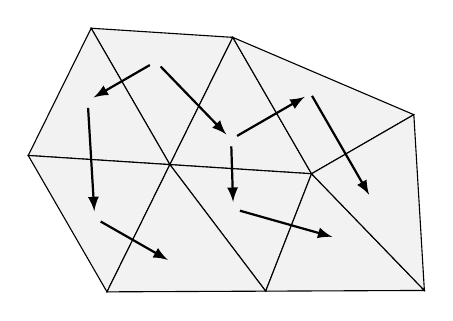
\begin{tikzpicture}[rotate=-60]
    \coordinate (A) at (0,0);
    \coordinate (B) at (2,0);
    \coordinate (C) at (1,1.5);
    \coordinate (D) at (3,1.5); 
    \coordinate (E) at (3,3); 
    \coordinate (F) at (4,0.25); 
    \coordinate (X) at (1,-1.5);
    \coordinate (Y) at (3,-1.5); 
    \coordinate (T) at (5,2); 
    
    \coordinate (CentroidABC) at ($(A)!0.3333!(B)!0.3333!(C)$);
    \coordinate (CentroidBCD) at ($(B)!0.3333!(C)!0.3333!(D)$);
    \coordinate (CentroidCDE) at ($(C)!0.3333!(D)!0.3333!(E)$);
    \coordinate (CentroidBDF) at ($(B)!0.3333!(D)!0.3333!(F)$);
    \coordinate (CentroidABX) at ($(A)!0.3333!(B)!0.3333!(X)$);
    \coordinate (CentroidBXY) at ($(Y)!0.3333!(B)!0.3333!(X)$);
    \coordinate (CentroidBFY) at ($(Y)!0.3333!(B)!0.3333!(F)$);
    \coordinate (CentroidDFT) at ($(D)!0.3333!(F)!0.3333!(T)$);
    \coordinate (CentroidDET) at ($(D)!0.3333!(E)!0.3333!(T)$);
    
    \draw[fill=gray!10] (A) -- (B) -- (C) -- cycle; 
    \draw[fill=gray!10] (B) -- (C) -- (D) -- cycle; 
    \draw[fill=gray!10] (C) -- (D) -- (E) -- cycle; 
    \draw[fill=gray!10] (B) -- (D) -- (F) -- cycle; 
    \draw[fill=gray!10] (A) -- (B) -- (X) -- cycle; 
    \draw[fill=gray!10] (Y) -- (B) -- (X) -- cycle; 
    \draw[fill=gray!10] (Y) -- (B) -- (F) -- cycle; 
    \draw[fill=gray!10] (T) -- (D) -- (F) -- cycle; 
    \draw[fill=gray!10] (T) -- (D) -- (E) -- cycle; 
    
    \draw[-latex, thick, shorten <=2.5pt, shorten >=2.5pt] (CentroidABC) -- (CentroidBCD); 
    \draw[-latex, thick, shorten <=2.5pt, shorten >=2.5pt] (CentroidBCD) -- (CentroidCDE); 
    \draw[-latex, thick, shorten <=2.5pt, shorten >=2.5pt] (CentroidBCD) -- (CentroidBDF); 
    \draw[-latex, thick, shorten <=2.5pt, shorten >=2.5pt] (CentroidABC) -- (CentroidABX); 
    \draw[-latex, thick, shorten <=2.5pt, shorten >=2.5pt] (CentroidABX) -- (CentroidBXY); 
    \draw[-latex, thick, shorten <=2.5pt, shorten >=2.5pt] (CentroidBXY) -- (CentroidBFY); 
    \draw[-latex, thick, shorten <=2.5pt, shorten >=2.5pt] (CentroidBDF) -- (CentroidDFT); 
    \draw[-latex, thick, shorten <=1.0pt, shorten >=2.0pt] (CentroidCDE) -- (CentroidDET); 
\end{tikzpicture}
\end{center}
\caption{Face-connected triangulation of a domain. The arrows depict a spanning tree in the face-connection graph.}
\label{figure:spanningtree}
\end{figure}


\begin{theorem}\label{theorem:poincarefriedrichsestimate:grad}
    Let $\calT$ be a face-connected $n$-dimensional finite triangulation. 
    Suppose $1 \leq p,q \leq \infty$ with $1 = 1/p + 1/q$,
    and that the domain $\Omega$ is the interior of the underlying set of $\calT$. 
    Then for any $u \in W^{1,p}(\Omega)$ 
    there exists $w \in W^{1,p}(\Omega)$ with $\nabla w = \nabla u$ 
    and satisfying the following estimates:
    there exists an $n$-simplex $T_0 \in \calT$ with 
    \begin{gather*}
        \| w_0 \|_{L^{p}(T_{0})} \leq C_{{\PF},T_{0},p} \| \nabla u \|_{L^{p}(T_{0})}.
    \end{gather*}
    and whenever $T_0, T_1, \dots, T_M$ is a face path,
    then for all $1 \leq m \leq$ we the following recursive estimates:
    \begin{align*}
        \| w \|_{L^{p}(T_{m})}
        &
        \leq  
        \volumeratio(\calT)^{\frac 1 p} 
        \| w \|_{L^{p}(T_{m-1})} 
        + 
%         C_{\PF,T_{m},F_{m},p} 
%         \left( 
%             \| \nabla u \|_{L^{p}(T_{m})} 
%             + 
%             \volumeratio(\calT)^{\frac 1 p} \reflectionestimate(\calT)
%             \| \nabla u \|_{L^{p}(T_{m-1})}
%         \right)
        \left( 1 + \volumeratio(\calT)^{\frac q p} \reflectionestimate(\calT)^{q} \right)^{\frac 1 q}
        C_{\PF,T_{m},F_{m},p} 
        \| \nabla u \|_{L^{p}(\Makoto_{F_m})} 
        ,
        \\
        \| w \|_{L^{p}(T_m)}
        &\leq 
        \volumeratio(\calT)^{\frac 1 p} 
        \| w \|_{L^{p}(T_{{m-1}})}
        +
        \left( 1 + \volumeratio(\calT)^{\frac q p} \right)^{\frac 1 q}
        C_{{\PF},\Makoto_{F_m},p} 
        \| \nabla u \|_{L^{p}(\Makoto_{F_m})} 
        . 
    \end{align*}
    Here, for any $1 \leq m \leq M$, let $F_m = T_m \cap T_{m-1}$.
\end{theorem}




\begin{proof}
    Let $u \in W^{1,p}(\Omega)$. 
    We start with the Poincar\'e--Friedrichs inequality on the first simplex $T_{0}$. 
    There exists $w_0 \in W^{1,p}(T_{0})$ satisfying $\nabla w_0 = \nabla u$ over $T_{0}$ together with 
    \begin{gather*}
        \| w_0 \|_{L^{p}(T_{0})} \leq C_{{\PF},T_{0},p} \| \nabla u \|_{L^{p}(T_{0})}.
    \end{gather*}
    In particular, $c_{0} := w_0 - u$ is a constant function. 
    We then define 
    \begin{align*}
        w := u + c_0
        .
    \end{align*} 
    Clearly, $w \in W^{1,p}(\Omega)$ with $\nabla w = \nabla u$.
    By construction $w_{|T_{0}} = w_0$. 
    We verify that $w$ satisfies the two desired recursive estimates.
    Suppose that $T_0, T_1, \dots, T_M$ is a face path in $\calT$
    and that $1 \leq m \leq M$.
    Recall that we write $F_m := T_m \cap T_{m-1}$, which is a face of dimension $n-1$ shared by the $n$-simplices $T_{m}$ and $T_{m-1}$,
    and that we write $\Makoto_{F_m} := T_m \cup T_{m-1}$. 
    
    We proceed with the first recursive estimate. 
    We define $w'_{m} := w_{|T_{m-1}} \circ \Xi \in W^{1,p}(T_{m})$,
    where $\Xi : T_{m} \rightarrow T_{m-1}$ is the unique affine diffeomorphism that leaves $F_{m}$ invariant. 
    By construction, $w'_{m} \in W^{1,p}(T_{m})$ with 
    \begin{align*}
        \trace_{F_{m}} w'_{m} = \trace_{F_{m}} w_{|T_{m-1}}
        .
    \end{align*}
    We now define $w''_{m} \in W^{1,p}(T_{m})$ via 
    \begin{align}\label{equation:w''}
        w''_{m} 
        := 
%         u_{|T_{m}} - w'_{m} + c_0 
%         = 
        w_{|T_{m}} - w'_{m} = u_{|T_{m}} - u_{|T_{m-1}} \circ \Xi.
    \end{align}
    We crucially note that $w''_{m}$ is trace-free along $F_{m}$ since
    \begin{align*}
        \trace_{F_{m}} w''_{m} 
        = 
        \trace_{F_{m}} \left( 
            w_{|T_{m}} - w'_{m} 
        \right) 
        =
        \trace_{F_{m}} w_{|T_{m}}
        -
        \trace_{F_{m}} w_{|T_{m-1}}
        =
        \trace_{F_{m}} u_{|T_{m}}
        -
        \trace_{F_{m}} u_{|T_{m-1}}
%         = 
%         \trace_{F_{m}} \left( 
%             u_{|T_{m}} - w'_{m} + c_0 
%         \right) 
%         = 
%         \trace_{F_{m}} \left( 
%             u_{|T_{m-1}} - w_{|T_{m-1}} + c_0 
%         \right) 
        = 0.
    \end{align*}
    We apply Lemma~\ref{lemma:mixedbconsimplex} to the first expression in~\eqref{equation:w''}, which gives 
    \begin{align*}
        \| w''_{m} \|_{L^{p}(T_{m})} 
        &
        \leq 
        C_{\PF,T_{m},F_{m},p} 
        \left( 
            \| \nabla w \|_{L^{p}(T_{m})} 
            + 
            \| \nabla w'_{m} \|_{L^{p}(T_{m})} 
        \right) 
        \leq 
        C_{\PF,T_{m},F_{m},p} 
        \left( 
            \| \nabla u \|_{L^{p}(T_{m})} 
            + 
            \| \nabla w'_{m} \|_{L^{p}(T_{m})} 
        \right) 
        .
    \end{align*}
    Using Lemma~\ref{lemma:volumecomparison} as well as Definitions~\eqref{math:volumeratio} and~\eqref{math:reflectionmeasure}, we find 
    \begin{align*}
        \| \nabla w'_{m} \|_{L^{p}(T_{m})}
        &
        \leq 
        |\det(\Jacobian \Xi  )|^{-\frac 1 p} 
        \matnorm{ \Jacobian \Xi }
        \| \nabla w \|_{L^{p}(T_{m-1})}
        \\&
        \leq 
        \volumeratio(\calT)^{\frac 1 p} \reflectionestimate(\calT)
        \| \nabla w \|_{L^{p}(T_{m-1})}
        \\&
        =
        \volumeratio(\calT)^{\frac 1 p} \reflectionestimate(\calT)
        \| \nabla u \|_{L^{p}(T_{m-1})}
        .
    \end{align*}
    % The second expression in~\eqref{equation:w''} shows $w_{|T_{m}} = w''_{m} + w'_{m}$. We finally find 
    Since $w_{|T_{m}} = w''_{m} + w'_{m}$, we finally find 
    \begin{align*}
        \| w \|_{L^{p}(T_{m})}
        &
        \leq  
        \| w'_{m} \|_{L^{p}(T_{m})}
        + 
        \| w''_{m} \|_{L^{p}(T_{m})}
        \\&
        \leq  
        \volumeratio(\calT)^{\frac 1 p} 
        \| w \|_{L^{p}(T_{m-1})} 
        + 
        C_{\PF,T_{m},F_{m},p} 
        \left( 
            \| \nabla u \|_{L^{p}(T_{m})} 
            + 
            \volumeratio(\calT)^{\frac 1 p} \reflectionestimate(\calT)
        \| \nabla u \|_{L^{p}(T_{m-1})}
        \right). 
    \end{align*}
    We now use H\"older's inequality. 
    Therefrom, the first recursive estimate follows.
    
    
    Now we discuss the second recursive estimate. 
    Suppose again that $1 \leq m \leq M$. 
    We use the Poincar\'e--Friedrichs inequality over $\Makoto_{F_{m}}$,
    as given in Lemma~\ref{lemma:poincarefriedrichsoverfacepatch}, 
    to find $w_{F_m} \in W^{1,p}(\Makoto_{F_m})$ such that $\nabla w_{F_m} = \nabla u$ over $\Makoto_{F_m}$ and 
    \begin{align}\label{math:wFm_inequality}
        \| w_{F_m} \|_{L^{p}(\Makoto_{F_m})} \leq C_{{\PF},\Makoto_{F_m},p} \| \nabla w_{F_m} \|_{L^{p}(\Makoto_{F_m})}.
    \end{align}
%     \cye{Since $\nabla (w_{|\Makoto_{F_m}}) = \nabla u_{F_{m}} = \nabla (u_{|\Makoto_{F_m}})$, 
    We can define the constant
    \begin{align*}
    c_{m} := w_{|\Makoto_{F_m}} - w_{F_{m}}.
    \end{align*}
    We now observe that 
    \begin{gather*}
        \| w \|_{L^{p}(T_m)}
        \leq 
        \| w_{F_m} \|_{L^{p}(T_m)}
        +
        \| c_{m} \|_{L^{p}(T_m)},
        \\
        \| c_{m} \|_{L^{p}(T_m)}
        = 
        \frac{ \vol(T_m)^{\frac 1 p} }{ \vol(T_{{m-1}})^{\frac 1 p} }
        \| c_{m} \|_{L^{p}(T_{{m-1}})},
        \\ 
        \| c_{m} \|_{L^{p}(T_{{m-1}})}
        \leq 
        \| w \|_{L^{p}(T_{{m-1}})} + \| w_{F_{m}} \|_{L^{p}(T_{{m-1}})} 
        .
    \end{gather*}
    In combination, 
    \begin{align*}
        \| w \|_{L^{p}(T_m)}
        &
        \leq 
        \| w_{F_m} \|_{L^{p}(T_m)}
        \\&\qquad 
        +
        \frac{ \vol(T_m)^{\frac 1 p} }{ \vol(T_{{m-1}})^{\frac 1 p} }
        \| w_{F_{m}} \|_{L^{p}(T_{{m-1}})}
        +
        \frac{ \vol(T_m)^{\frac 1 p} }{ \vol(T_{{m-1}})^{\frac 1 p} }
        \| w \|_{L^{p}(T_{{m-1}})}
        .
    \end{align*}
    We sum the two integrals of $w_{F_m}$. 
    % 
    % 1/q = 1 - 1/p = (p-1)/p 
    When $1 < p < \infty$, recalling the complementary exponent $q = p/(p-1) \in (1,\infty)$, 
    we use H\"older's inequality to verify 
    \begin{align*}
        \| w \|_{L^{p}(T_m)}
        &\leq 
        \left( 1 + \frac{ \vol(T_m)^{\frac q p} }{ \vol(T_{{m-1}})^{\frac q p} } \right)^{\frac 1 q}
        \left( 
            \| w_{F_{m}} \|_{L^{p}(T_m)}^{p}
            +
            \| w_{F_{m}} \|_{L^{p}(T_{{m-1}})}^{p}
        \right)^{\frac 1 p}
        +
        \frac{ \vol(T_m)^{\frac 1 p} }{ \vol(T_{{m-1}})^{\frac 1 p} }
        \| w \|_{L^{p}(T_{{m-1}})}
        \\&\leq 
        \left( 1 + \frac{ \vol(T_m)^{\frac q p} }{ \vol(T_{{m-1}})^{\frac q p} } \right)^{\frac 1 q}
        \| w_{F_{m}} \|_{L^{p}(\Makoto_{F_m})} 
        +
        \frac{ \vol(T_m)^{\frac 1 p} }{ \vol(T_{{m-1}})^{\frac 1 p} }
        \| w \|_{L^{p}(T_{{m-1}})}
        .
    \end{align*}
    Note that in the limit cases $p=1$ and $p=\infty$ we get, respectively, 
    \begin{align*}
        \| w\|_{L^{1}(T_m)}
        &\leq 
        \max\left(
            1, \frac{ \vol(T_m) }{ \vol(T_{{m-1}}) } 
        \right)
        \| w_{F_m} \|_{L^{1}(\Makoto_{F_m})}
        +
        \frac{ \vol(T_m) }{ \vol(T_{{m-1}}) }
        \| w \|_{L^{1}(T_{{m-1}})},
        \\
        \| w \|_{L^{\infty}(T_m)}
        &\leq 
        2
        \| w_{F_m} \|_{L^{\infty}(\Makoto_{F_m})}
        +
        \| w \|_{L^{\infty}(T_{{m-1}})}
        .
    \end{align*}
    The local inequality~\eqref{math:wFm_inequality} now provides the second recursive estimate. 
    The proof is complete.
\end{proof}


\begin{corollary}
    Under the assumptions of Theorem~\ref{theorem:poincarefriedrichsestimate:grad},
    whenever $T_0, T_1, \dots, T_m$ is a face-path of $n$-simplices in $\calT$,
    we have 
    \begin{align*}
        \| w \|_{L^{p}(T_m)}
        &\leq 
        \sum_{\ell=1}^{m} 
        \volumeratio^{\frac{m-\ell}{p}}
        \min\left( 
        \left( 1 + \volumeratio(\calT)^{\frac q p} \right)^{\frac 1 q}
        C_{{\PF},\Makoto_{F_\ell},p} 
        ,
        \left( 1 + \volumeratio(\calT)^{\frac q p} \reflectionestimate(\calT)^{q} \right)^{\frac 1 q}
        C_{\PF,T_{\ell},F_{\ell},p} 
        \right)
        \| \nabla u \|_{L^{p}(\Makoto_{F_\ell})}
        \\&
        \qquad 
        \qquad 
        +
        \volumeratio^{\frac m p}
        C_{{\PF},T_{0},p}
        \| \nabla u \|_{L^{p}(T_{0})}
        .
    \end{align*}
\end{corollary}
\begin{proof}
    This follows by repeated application of the recursive estimate in Theorem~\ref{theorem:poincarefriedrichsestimate:grad}.
\end{proof}


\begin{remark}
    The Poincar\'e--Friedrichs constants obtained from Theorem~\ref{theorem:poincarefriedrichsestimate:grad} increasingly overestimate the best one as the number of $n$-simplices in the triangulation $\calT$ increases. 
    Hence, we conceive their target application to be local patches (stars), in particular non-convex boundary stars. 
    The latter occur inevitably at reentrant corners. Clearly, the same building principle applies whenever we have any non-overlapping partition of $\overline \Omega$ into convex local patches $\{ \Makoto_m \}$ of $n$-simplices with an appropriate notion of connectivity. 
    The proof proceeds verbatim, where we merely replace the simplices $\{ T_{m} \}$ by the convex local patches $\{ \Makoto_m \}$. 
    This may allow for partitions of $\overline \Omega$ with significantly fewer elements, which enables a largely improved estimate of the best Poincar\'e--Friedrichs constant. 
\end{remark}


% https://people.tamu.edu/~guermond//PUBLICATIONS/ern_guermond_m2an_2016.pdf 
% Lemma 5.5

    























\section{Review of vector calculus and exterior calculus}\label{section:calculus}

% We discuss the Sobolev spaces of vector calculus and exterior calculus 
% with particular emphasis on their transformation behavior. 
% We refer the reader to Ern and Guermond~\cite{ern2021finite} and Hiptmair~\cite{hiptmair2002finite} for further background material on Sobolev vector analysis. 
% Exterior algebra and exterior products are reviewed in the textbooks by Greub~\cite{greub1967multilinear} and Lee~\cite{lee2012smooth}.
% TODO: Fuse these two paragraphs 

We review in this section the Sobolev spaces of vector and exterior calculus and their transformation behavior. We refer the reader to Ern and Guermond~\cite{ern2021finite} and Hiptmair~\cite{hiptmair2002finite} for background material on Sobolev vector analysis and to Greub~\cite{greub1967multilinear} and Lee~\cite{lee2012smooth} for exterior algebra and exterior products. 

\subsection{Vector calculus}

% \cye{Recall the notations~\eqref{equation:W1p} and~\eqref{equation:W_curl_div_p} from Section~\ref{section:intro}; actually, here we temporarily rather employ 
% \begin{gather*}
    % W^{p}(\grad,\Omega) \cye{= W^{1,p}(\Omega)} = \{ u \in L^{p}(\Omega) \suchthat \grad v \in \bfL^{p}(\Omega) \}
    % .
% \end{gather*}}
Let $\Omega \subseteq \bbR^{3}$ be a bounded open set. 
We recall $L^{p}(\Omega)$, the space of scalar-valued $p$-integrable functions defined on $\Omega$
and that $\bfL^{p}(\Omega) := L^{p}(\Omega)^{n}$ for vector-valued functions with each component in $L^{p}(\Omega)$. 
In the three-dimensional setting, we are particularly interested in the Sobolev vector analysis. 
The space of scalar-valued $L^{p}(\Omega)$ functions with weak gradients in $\bfL^{p}(\Omega)$ is 
\begin{gather*}
    W^{p}(\grad,\Omega) := W^{1,p}(\Omega) = \{ u \in L^{p}(\Omega) \suchthat \grad v \in \bfL^{p}(\Omega) \}
    .
\end{gather*}
The space $\bfW^{p}(\curl,\Omega)$ of vector-valued $\bfL^{p}(\Omega)$ functions with weak curls in $\bfL^{p}(\Omega)$
and the space of vector-valued $\bfL^{p}(\Omega)$ functions with weak divergences in $L^{p}(\Omega)$ are written 
\begin{gather*}
    \bfW^{p}(\curl,\Omega) = \{ \bfu \in \bfL^{p}(\Omega) \suchthat \curl \bfu \in \bfL^{p}(\Omega) \},
    \\ 
    \bfW^{p}(\divergence,\Omega) = \{ \bfu \in \bfL^{p}(\Omega) \suchthat \divergence \bfu \in L^{p}(\Omega) \}.
\end{gather*}
We are interested in transformations of these Sobolev tensor fields from one domain onto another. 
Suppose that $\Omega, \Omega' \subset \mathbb{R}^3$ are open sets and suppose that $\phi: \Omega \to \Omega'$ is a bi-Lipschitz mapping.
We introduce the gradient-, curl-, and divergence-conforming Piola transformations, respectively, as the mappings 
$\phi^{\grad}: L^{p}(\Omega') \to L^{p}(\Omega)$,
$\phi^{\curl}: \bfL^{p}(\Omega') \to \bfL^{p}(\Omega)$, and 
$\phi^{\divergence}: \bfL^{p}(\Omega') \to \bfL^{p}(\Omega)$.
We also introduce 
$\phi^{\rm b}: L^{p}(\Omega') \to L^{p}(\Omega)$. 
We define them 
for any $v \in L^{p}(\Omega')$ and $\bfw \in \bfL^{p}(\Omega')$ by setting 
\begin{subequations}\label{eq_definition_piola}
\begin{align*}
    \phi^{\grad}(v) &= v \circ \phi, \\
    \phi^{\curl}(\bfw) &= \Jacobian\phi^{T} (\bfw \circ \phi), \\
    \phi^{\divergence}(\bfw) &= \adj(\Jacobian\phi) \left( \bfw \circ \phi \right), \\  
    \phi^{\rm b}(v) &= \det(\Jacobian\phi) \left( v \circ \phi \right),
\end{align*}
\end{subequations}
Here, $\Jacobian\phi$ is the Jacobian matrix of $\phi$ (see also~\cite[Definition~9.8]{ern2021finite}), and $\adj\Jacobian\phi$ denotes taking its adjugate matrix.
These transformations are invertible. 
Bounds on the Lebesgue norms will follow from a more general result below. 
We use the commutativity relations 
\begin{subequations}\label{eq_piola_commute}
\begin{align}
    \grad \phi^{\grad} (v) &= \phi^{\curl}(\grad v), 
    \\
    \curl \phi^{\curl}(\bfv) &= \phi^{\divergence}(\curl \bfv), 
    \\
    \divergence \phi^{\divergence}(\bfw) &= \phi^{\rm b}(\divergence \bfw),
\end{align}
\end{subequations}
where $v \in W^{p}(\grad,\Omega)$, $\bfv \in \bfW^{p}(\curl,\Omega)$, and $\bfw \in \bfW^{p}(\divergence,\Omega)$.  
We summarize this as a commuting diagram:
\begin{align*}
    \begin{CD}
        W^{p}(\grad,\Omega') @>{\grad}>> \bfW^{p}(\curl,\Omega') @>{\curl}>> \bfW^{p}(\divergence,\Omega') @>{\divergence}>> L^{p}(\Omega')
        \\
        @VV{\phi^{\grad}}V 
        @VV{\phi^{\curl}}V 
        @VV{\phi^{\divergence}}V 
        @VV{\phi^{\rm b}}V 
        \\
        W^{p}(\grad,\Omega ) @>{\grad}>> \bfW^{p}(\curl,\Omega ) @>{\curl}>> \bfW^{p}(\divergence,\Omega ) @>{\divergence}>> L^{p}(\Omega ).
    \end{CD}
\end{align*}

\begin{remark}
    The Piola transform goes into the opposite direction of the mapping $\phi : \Omega \rightarrow \Omega'$:
    scalar and vector fields over $\Omega'$ are transformed into scalar and vector fields over $\Omega$.
    This definition is in accordance with the notion of pullback, which we will review shortly. 
    One advantage of that definition is that it also makes sense whenever the transformation is not bijective. 
    However, the literature also knows the Piola transform in the direction of the original mapping. 
\end{remark}


\subsection{Exterior calculus}

%\cye{We now move to} exterior calculus. 
%We give a brief introduction into this topic, and refer to the literature for further background~\cite{lee2012smooth}. 

We now move the discussion to exterior calculus, beginning with exterior algebra.
Let $V$ be a real vector space. 
Given an integer $k \geq 0$, we let $\Alt^{k}(V)$ denote the space of scalar-valued antisymmetric $k$-linear forms over $V$. 
Recall that any $k$-linear scalar-valued form $u$ over $V$ is called antisymmetric
if 
\begin{gather*} 
    u( v_{\pi(1)}, v_{\pi(2)}, \ldots, v_{\pi(k)} ) 
    = 
    \text{sign}(\pi) 
    u( v_1, v_2, \ldots, v_k ) 
\end{gather*}
for any $v_1, v_2, \dots, v_k \in V$ and any permutation $\pi$ of the indices \(\{1, 2, \ldots, k\}\). 
By definition, $\Alt^{1}(V)$ is just the dual space of $V$, and $\Alt^{0}(V)$ is the space of real numbers. 
Formally, we define $\Alt^{k}(V)$ to be the zero vector space when $k < 0$. 

The wedge product (or exterior product) of alternating multilinear forms is a fundamental operation in exterior algebra
(see~Chapter 14 in \cite{lee2012smooth}). 
Given two alternating multilinear forms \( u_1 \in \Alt^{k}(V) \) and \( u_2 \in \Alt^{l}(V) \), 
their wedge product \( u_1 \wedge u_2 \) is a member of $\Alt^{k+l}(V)$
defined by the formula 
\begin{gather*}
    (u_1 \wedge u_2)(v_1, v_2, \ldots, v_{k+l}) 
    = 
    \frac{1}{k! l!} 
    % \sum_{ \pi \in S_{k+l}} 
    \sum_{ \pi } 
    \signum(\pi) 
    u_1( v_{\pi(  1)}, \ldots, v_{\pi(k  )} ) 
    u_2( v_{\pi(k+1)}, \ldots, v_{\pi(k+l)} ),
\end{gather*}
for any \( v_1, v_2, \ldots, v_{k+l} \in V \).
Here, the sum runs over all permutations $\pi$ of the index set \(\{ 1, 2, \ldots, k+l \}\).
% Here, \( S_{k+l} \) denotes the symmetric group on \( k+l \) elements, and \( \signum(\pi) \) is the sign of the permutation \( \pi \). 
The exterior product is bilinear and associative, and satisfies 
\begin{align*}
    u_1 \wedge u_2 = (-1)^{kl} u_2 \wedge u_1,
    \quad 
    \forall u_1 \in \Alt^{k}(V),
    \quad 
    \forall u_2 \in \Alt^{l}(V).
\end{align*}
The interior product is in some sense dual to the exterior product. Given $v \in V$ and $u \in \Alt^{k}(V)$, we define the interior product $v \lrcorner u \in \Alt^{k-1}(V)$ via 
\begin{align*}
    (v \lrcorner u)( v_1, v_2, \ldots, v_{k-1} ) = u( v, v_1, v_2, \ldots, v_{k-1} ),
    \quad 
    \forall v_1, v_2, \ldots, v_{k-1} \in V.
\end{align*}

We employ the exterior algebra only in the special case $V = \bbR^{n}$ of alternating forms over the $n$-dimensional Euclidean space. 
Here, it is customary to identify $\Alt^{k}(V)$ with the space of antisymmetric tensors in $k$ indices. 
Moreover, this particular setting comes with a canonical basis. 
We let \(\{\cartanx^1, \cartanx^2, \ldots, \cartanx^{n}\}\) be the basis dual to the canonical unit vectors.
This is a canonical basis of $\Alt^{1}(\bbR^{n})$. 
To define a canonical basis of $\Alt^{k}(\bbR^{n})$, 
we first introduce $\Sigma(k,n)$, the set of strictly ascending mappings $\sigma : \{1,\dots,k\} \rightarrow \{1,\dots,n\}$, where $k, n \in \bbZ$, 
and introduce the basic $k$-alternators 
\begin{align*}
    \cartanx^{\sigma} := \cartanx^{\sigma(1)} \wedge \dots \wedge \cartanx^{\sigma(k)}, 
    \quad 
    \forall \sigma \in \Sigma(k,n). 
\end{align*}
These define a basis of $\Alt^{k}(\bbR^{n})$.
Note that 
$\dim \Alt^{k}(\bbR^{n}) = \binom{n}{k}$. 
In particular, $\Alt^{k}(\bbR^{n})$ is the zero vector space whenever $k > n$.
% The dimension of the space of \(k\)-forms, denoted \(\bigwedge^{k} V\), is given by the binomial coefficient \(\binom{n}{k}\).

We notice that the canonical scalar product on $\bbR^{n}$ gives rise to a scalar product on $\Alt^{1}(\bbR^{n})$,
which induces a scalar product on $\Alt^{k}(\bbR^{n})$.
The basic $k$-alternators are an orthonormal basis of $\Alt^{k}(\bbR^{n})$ with respect to that inner product. 

\subsection{Smooth differential forms}

We let $\Omega \subseteq \bbR^{n}$ be any bounded open set.
We write $C^{\infty}\Alt^{k}(\Omega)$ for the space of smooth differential $k$-forms over $\Omega \subseteq \bbR^{n}$,
which is the vector space of smooth mappings from $\Omega$ into $\Alt^{k}(\bbR^{n})$.
The exterior derivative \( \cartan \) is an operator that takes a \( k \)-form \( \omega \in C^{\infty}\Alt^{k}(\Omega) \) 
to a \((k+1)\)-form \( \cartan\omega \in C^{\infty}\Alt^{k+1}(\Omega) \). 
Every \( k \)-form \( \omega \in C^{\infty}\Alt^{k}(\Omega) \) can be written 
\begin{gather*}
    \omega 
    = 
    \sum_{ \sigma \in \Sigma(k,n) } 
    \omega_{\sigma} \, 
    \cartanx^{\sigma}
    = 
    \sum_{ \sigma \in \Sigma(k,n) } 
    \omega_{\sigma} \, 
    \cartanx^{\sigma(1)} \wedge \cartanx^{\sigma(2)} \wedge \cdots \wedge \cartanx^{\sigma(k)},
\end{gather*}
where \( \omega_{\sigma} : \Omega \rightarrow \bbR \) are smooth functions.
The exterior derivative \( \cartan\omega \) is defined by
\begin{gather*}
    \cartan\omega = 
    \sum_{ \sigma \in \Sigma(k,n) } 
    \sum_{j=1}^{n} 
    \frac{\partial \omega_{\sigma}}{\partial x^j} 
    \, \cartanx^j \wedge 
    \cartanx^{\sigma(1)} \wedge \cartanx^{\sigma(2)} \wedge \cdots \wedge \cartanx^{\sigma(k)}.
\end{gather*}
The exterior derivative is linear and nilpotent, which means 
\( \cartan(\cartan\omega) = 0 \) for any \( \omega \in C^{\infty}\Alt^{k}(\Omega) \).
Moreover, it satisfies the Leibniz rule:
\begin{gather*} 
    \cartan(\omega \wedge \eta) 
    = 
    \cartan\omega \wedge \eta + (-1)^{k} \omega \wedge \cartan\eta, 
    \qquad \forall \omega \in C^{\infty}\Alt^{k}(\Omega), 
    \qquad \forall \eta \in C^{\infty}\Alt^{l}(\Omega).
\end{gather*}
The integral of a differential $n$-form is uniquely defined via 
\begin{gather*}
    \int_{\Omega} \omega \cartanx^{1} \wedge \dots \wedge \cartanx^{n} = \int_{\Omega} \omega(x) \;dx
    . 
\end{gather*}



\begin{remark}
    In three dimensions, 
    the calculus of differential forms is in correspondence with classical vector calculus. 
    This is expressed formally as the commuting diagram 
    \begin{gather*}
    \begin{CD}
        C^\infty\Alt^0(\Omega) @>{\cartan}>> C^\infty\Alt^1(\Omega) @>{\cartan}>> C^\infty\Alt^2(\Omega) @>{\cartan}>> C^\infty\Alt^3(\Omega) 
        \\
        @VV{\varpi^{0}}V 
        @VV{\varpi^{1}}V 
        @VV{\varpi^{2}}V 
        @VV{\varpi^{3}}V 
        \\
        C^\infty(\Omega) @>{\grad}>> C^\infty(\Omega)^{3} @>{\curl}>> C^\infty(\Omega)^{3} @>{\divergence}>> C^\infty(\Omega)
    \end{CD}
    \cye{\, ,}
    \end{gather*}
    where $\varpi^{0}$ and $\varpi^{3}$ are the identity mappings and where 
    \begin{align*}
     \varpi^{1}\left( u_1 \cartanx^{1} + u_2 \cartanx^{2} + u_3 \cartanx^{3} \right) 
     &= 
     \left( u_1, u_2, u_3 \right), 
     \\
     \varpi^{2}\left( u_{12} \cartanx^{1} \wedge \cartanx^{2} + u_{13} \cartanx^{1} \wedge \cartanx^{3} + u_{23} \cartanx^{2} \wedge \cartanx^{3} \right) 
     &= 
     \left( u_{23}, - u_{13}, u_{12} \right).   
    \end{align*}
    In two dimensions, 
    the calculus of differential forms can be translated into 2D vector calculus in two different ways. 
    To the authors' best knowledge, neither convention is dominant over the other in the literature.
    We summarize the situation in the following commuting diagram: 
    \begin{gather*} 
    \begin{CD}
        C^\infty(\Omega) @>{\curl}>> C^\infty(\Omega)^{2} @>{\divergence}>> C^\infty(\Omega)
        \\
        @AA{\varkappa^{0}}A 
        @AA{\varkappa^{1}}A 
        @AA{\varkappa^{2}}A 
        \\
        C^\infty\Alt^0(\Omega) @>{\cartan}>> C^\infty\Alt^1(\Omega) @>{\cartan}>> C^\infty\Alt^2(\Omega) 
        \\
        @VV{\varpi^{0}}V 
        @VV{\varpi^{1}}V 
        @VV{\varpi^{2}}V 
        \\
        C^\infty(\Omega) @>{\grad}>> C^\infty(\Omega)^{2} @>{\rot}>> C^\infty(\Omega)
    \end{CD}
    \cye{\,.}
    \end{gather*}
    Here, $\varpi^{1}\left( u_1 \cartanx^{1} + u_2 \cartanx^{2} \right) = \left( u_1, u_2 \right)$ is the lower middle isomorphism. We introduce the rotation operator $J(x,y) = (y,-x)$ and define $\varkappa = J \varpi$ and $\rot = \divergence J$.
    The other vertical arrows are the identity. 
    The utility of exterior calculus is that the operators of vector calculus can be translated into a common framework that does not depend on the dimension.
\end{remark}


\subsection{Sobolev spaces of differential forms}

Let us now turn our attention to Sobolev spaces of differential forms. 
Since the exterior product space $\Alt^{k}(\bbR^{n})$ carries a norm, induced from the Euclidean norm on $\bbR^{n}$, there are pointwise norms of differential $k$-forms. 
We let $L^{p}\Alt^{k}(\Omega)$ be the space of differential $k$-forms over $\Omega$ with locally integrable coefficients 
such that its pointwise norm is $p$-integrable. 
The exterior derivative is defined in the sense of distributions and we introduce 
\begin{gather*}
    W^{p}\Alt^{k}(\Omega) 
    := 
    \{ u \in L^{p}\Alt^{k}(\Omega) \suchthat \cartan u \in L^{p}\Alt^{k+1}(\Omega) \}
    .
\end{gather*}
We observe that $u \in L^{p}\Alt^{k}(\Omega)$ has weak exterior derivative $f \in L^{p}\Alt^{k+1}(\Omega)$
if and only if for all $v \in C^{\infty}_{c}\Lambda^{n-k-1}(\Omega)$ we have the integration by parts formula
\begin{align*}
    \int_{\Omega} \cartan v \wedge u
    &=
    (-1)^{k(n-k)+1}
    \int_{\Omega} v \wedge f 
    .
\end{align*}
% \mwl{We let $W^{p}_{0}\Alt^{k}(\Omega)$ be the closed subspace of those $u \in W^{p}\Alt^{k}(\Omega)$
% for which the extension by zero $\tilde u : \bbR^{n} \rightarrow \Alt^{k}(\bbR^{n})$ is a member of $\tilde u \in W^{p}\Alt^{k}(\bbR^{n})$.
% The space $W^{p}_{0}\Alt^{k}(\Omega)$ formalizes the idea of differential forms with vanishing boundary trace along the boundary $\partial\Omega$.}
% \cye{\sout{We let $W^{p}_{0}\Alt^{k}(\Omega)$ be the closed subspace of those $u \in W^{p}\Alt^{k}(\Omega)$ 
% for which the extension by zero $\tilde u : \bbR^{n} \rightarrow \Alt^{k}(\bbR^{n})$ is a member of $\tilde u \in W^{p}\Alt^{k}(\bbR^{n})$. }}\todo{MV: repeated below.}
Lastly, we are also interested in differential forms whose trace vanishes along a part of the boundary. 
Suppose that $\Gamma \subseteq \partial\Omega$ is a relatively open subset of the boundary. 
We say that $u \in W^{p}\Alt^{k}(\Omega)$ has vanishing trace along $\Gamma$ if for all $x \in \Gamma$ there exists $r > 0$
% such that for all $v \in C^{\infty}_{c}\Lambda^{n-k-1}(B_r(x))$ we have the integration by parts formula
such that for all $v \in C^{\infty}_{c}\Lambda^{n-k-1}(\bbR^{n})$ 
whose support lies in the open ball $B_r(x)$
we have the integration by parts formula
\begin{align*}
    \int_{B_r(x)} \cartan v \wedge \tilde u
    &=
    (-1)^{k(n-k)+1}
    \int_{B_r(x)} v \wedge \widetilde{\cartan u}
    .
\end{align*}
If that condition is satisfied, we also write 
\begin{align*}
    \trace_{\Gamma} u = 0
    .
\end{align*}
Accordingly, we write $\trace_{\Gamma} u = \trace_{\Gamma} u'$ for $\trace_{\Gamma} (u-u') = 0$ whenever $u, u' \in W^{p}\Alt^{k}(\Omega)$.
Lastly, we introduce the closed subspaces 
\begin{gather*}
    W^{p}_{0}\Alt^{k}(\Omega) 
    := 
    \{ u \in W^{p}\Alt^{k}(\Omega) \suchthat \trace_{\partial \Omega} u = 0 \}
    .
\end{gather*}
% \cye{The space $W^{p}_{0}\Alt^{k}(\Omega)$ formalizes the idea of differential forms with vanishing boundary trace along the boundary $\partial\Omega$.}\todo{MV: Moved here.}
This is a closed subspace. We know that $u \in W^{p}_{0}\Alt^{k}(\Omega)$ if and only if its extension by zero $\tilde u : \bbR^{n} \rightarrow \Alt^{k}(\bbR^{n})$ is a member of $\tilde u \in W^{p}\Alt^{k}(\bbR^{n})$. Moreover, $\cartan W^{p}_{0}\Alt^{k}(\Omega) \subseteq W^{p}_{0}\Alt^{k+1}(\Omega)$. We also observe that $W^{p}\Alt^{n}(\Omega) = W^{p}_{0}\Alt^{n}(\Omega) = L^{p}(\Omega)$. We use the abbreviation $W^{1,p}_{0}(\Omega) := W^{p}\Lambda^{0}(\Omega)$. 


\subsection{Transformations by bi-Lipschitz mappings}

We are interested in transformations of Sobolev tensor fields from one domain onto another. 
Suppose that $\Omega,\Omega' \subset \bbR^{n}$ are open sets and suppose that $\phi: \Omega \to \Omega'$ is a bi-Lipschitz mapping.
The pullback of $u \in L^{p}\Alt^{k}(\Omega')$ along $\phi$ is the (measurable) differential form 
\begin{align} \label{equation:pullback}
    \phi^{\ast}u_{|x}( v_{1}, v_{2}, \ldots, v_{k} ) 
    := 
    u_{|\phi(x)}( \Jacobian\phi_{|x} \cdot v_1, \Jacobian\phi_{|x} \cdot v_2, \ldots, \Jacobian\phi_{|x} \cdot v_k ) 
\end{align}
for any $v_1, v_2, \dots, v_k \in \bbR^{n}$ and any $x \in \Omega$. 
One can show that $\phi^{\ast}u \in L^{p}\Alt^{k}(\Omega)$ and the following estimates.

\begin{proposition}\label{proposition:pullbackestimate}
    Let $\phi : \Omega \rightarrow \Omega'$ be a bi-Lipschitz mapping between open sets $\Omega, \Omega' \subseteq \bbR^{n}$.
    Let $p \in [1,\infty]$ and $u \in L^{p}\Lambda^{k}(\Omega')$. 
    Then $\phi^{\ast} u \in L^{p}\Lambda^{k}(\Omega)$ and 
    \begin{align}
        \| \phi^{\ast} u \|_{L^{p}\Lambda^{k}(\Omega)}
        &\leq 
        \| \Jacobian \phi \|^{k}_{L^{\infty}(\Omega)}
        \| \det\Jacobian \phi^{-1} \|^{\frac{1}{p}}_{L^{\infty}(\Omega')}
        \| u \|_{L^{p}\Lambda^{k}(\Omega')}
        .
    \end{align}
    If $\phi$ is affine and $\sigma_1 \geq \sigma_2 \geq \dots \geq \sigma_n$ are the singular values of $\Jacobian\phi$, then 
    \begin{align}
        \| \phi^{\ast} u \|_{L^{p}\Lambda^{k}(\Omega)}
        &\leq 
        \sigma_1 \sigma_2 \cdots \sigma_k \cdot 
        \| \det\Jacobian \phi^{-1} \|^{\frac{1}{p}}_{L^{\infty}(\Omega')}
        \| u \|_{L^{p}\Lambda^{k}(\Omega')}
        .
    \end{align}
	Moreover, if $u \in W^{p}\Lambda^{k}(\Omega')$, then $\phi^{\ast} u \in W^{p}\Lambda^{k}(\Omega)$ and $\cartan \phi^{\ast} u = \phi^{\ast} \cartan u$. 
\end{proposition}
\begin{proof}
	See~\cite{licht2019smoothed} and Corollary~6 in~\cite{stern2013lp}).
\end{proof}




\subsection{Some approximation properties}

We review a few approximation properties. 
Let $\mollifier$ be a non-negative scalar function whose integral equals one and whose support lies in the unit ball around the origin.
Define $\mollifier_{\eps}(x) := \eps^{-n} \mollifier(x/\eps)$. We review the following approximation results.

\begin{lemma}
%     Let $\Omega \subseteq \bbR^{n}$ be a bounded open set and let $u : \Omega \rightarrow \bbR$ be locally integrable.  
%     Then $\mollifier_{\epsilon} \star u \rightarrow u$ almost everywhere. 
%     If $u \in L^{p}(\Omega)$ for some $1 \leq p < \infty$, then $u_{\epsilon} \rightarrow u$ in $L^{p}(\Omega)$.
    Let $\Omega \subseteq \bbR^{n}$ be a bounded open set and let $1 \leq p < \infty$. 
    If $u \in L^{p}(\Omega)$, then the convolution $\mollifier_{\eps} \star u \rightarrow u$ in $L^{p}(\Omega)$ as $\epsilon \rightarrow 0$.
\end{lemma}

% \begin{lemma} % TODO: possibly useful
%     Let $1 \leq p < \infty$. A sequence converges to $u \in L^{p}$ if and only if it converges locally by measure and the $L^{p}$ norms converge.
% \end{lemma}

\begin{lemma}
    Let $\Omega \subseteq \bbR^{n}$ be a bounded open set and let $1 \leq p < \infty$. 
    Smooth forms are dense in $W^{p}\Lambda^{k}(\Omega)$.
    If $\Omega$ is convex, then $C^{\infty}_{c}\Lambda^{k}(\Omega)$ is dense in $W^{p}_{0}\Lambda^{k}(\Omega)$. 
    %\mwl{If $\Omega$ is convex and $u \in W^{p}\Lambda^{n}(\Omega)$ has average zero, 
    %then $u$ is the limit in $W^{p}\Lambda^{k}(\Omega)$ of smooth compactly supported $n$-forms with average zero.}
\end{lemma}
\begin{proof}
    We notice $\mollifier_{\epsilon} \star u \in C^{\infty}\Lambda^{k}(\bbR^{n})$. 
    By the dominated convergence theorem and because $u$ has a weak derivative,
    for any $v \in C^{\infty}_{c}\Lambda^{n-k-1}(\Omega)$
    \begin{align*}
        \int_{\bbR^{n}} ( \mollifier_{\epsilon} \star u ) \wedge \cartan v 
        &= 
        \int_{\bbR^{n}} \int_{\bbR^{n}} \mollifier(x-y) \wedge u(y) \wedge \cartan_{x} v(x) \;dx\,dy
        \\&= 
        \int_{\bbR^{n}} \int_{\bbR^{n}} \cartan_x\mollifier(x-y) \wedge u(y) \wedge v(x) \;dx\,dy
        \\&= 
        - \int_{\bbR^{n}} \int_{\bbR^{n}} \cartan_y\mollifier(x-y) \wedge u(y) \wedge v(x) \;dx\,dy
        \\&= 
        \int_{\bbR^{n}} \int_{\bbR^{n}} \mollifier(x-y) \wedge \cartan_y u(y) \wedge v(x) \;dx\,dy
        = 
        \int_{\bbR^{n}} ( \mollifier_{\epsilon} \star \cartan u ) \wedge v 
        .
    \end{align*}
    Hence $C^{\infty}\Lambda^{k}(\Omega)$ is dense in $W^{p}\Lambda^{k}(\Omega)$.
    
    Next, suppose that $\Omega$ is convex. Without loss of generality, $0 \in \Omega$. 
    Let $u \in W^{p}_{0}\Lambda^{k}(\Omega)$ and extend $u$ trivially onto $\bbR^{n}$. 
    Define $\varphi_t(x) = tx$ for $t > 1$. 
    Then $\varphi_{t}^{\ast} u \in W^{p}_{0}\Lambda^{k}(t^{-1}\Omega) \subseteq W^{p}_{0}\Lambda^{k}(\Omega)$ 
    and $\varphi_{t}^{\ast} u$ converges to $u$ as $t$ decreases towards $1$. 
    Given any $t > 1$, by taking the convolution with $\mollifier_{\epsilon}$ for $\epsilon > 0$ small enough,
    we approximate $\varphi_{t}^{\ast} u$ through members of $C^{\infty}_{c}\Lambda^{k}(\Omega)$.
    The desired result follows. 
    % 
    % Lastly, if $k = n$ and $u$ has average zero, then so do the $\varphi_{t}^{\ast} u$ and their mollifications with sufficiently small radius. The proof is complete. 
\end{proof}
















\section{Regularized potential operators over convex sets}\label{section:potentialoperator}


% We want to bound Poincar\'e--Friedrichs constants for the exterior derivative over convex domains.
% We already know the optimal constants for the gradient operator over convex domains,
% and we know bounds for the Poincar\'e--Friedrichs constants for the entire $L^{2}$ de~Rham complex. 
% We are not aware of such bounds for the case of the $L^{p}$ de~Rham complex when $1 \leq p \leq \infty$. 
% % 
% We bound the norms of regularized potential operators for the exterior derivative over convex domains.
% We solve this for two special cases: 

We now develop bounds for Poincar\'e--Friedrichs constants for the exterior derivative over convex domains.
Here, we consider two special cases: 
either the $L^{p}$ de~Rham complex without boundary conditions, or the $L^{p}$ de~Rham with full boundary conditions. 
The corresponding potential operators are known as the regularized Poincar\'e and regularized Bogovski\u{\i} potentials in the literature. 
We build upon the discussion spearheaded by Costabel and McIntosh~\cite{costabel2010bogovskiui},
who analyze them as pseudo-differential operators over domains star-shaped with respect to a ball. 
% 
In comparison to their extensive work, our discussion is more modest:
we study potential operators merely over convex sets, and we are only interested in their operator norms between Lebesgue spaces.
However, our goal is explicit bounds for the operator norms, giving the Poincar\'e--Friedrichs constants. 

%\mwl{In what follows, $\Omega \subseteq \bbR^{n}$ is a convex bounded open set with diameter $\diam(\Omega) > 0$.}
Let $\Omega \subseteq \bbR^{n}$ is a convex bounded open set with diameter $\diam(\Omega) > 0$.

% \todo{MV: Discussion already in the introduction, or in Remark~\ref{remark:reg_Poinc_Bog}}: 








\subsection{Regularized Poincar\'e and Bogovski\u{\i} operators}

We begin with introducing the Costabel-McIntosh kernel.
For any $\mia \in \{0,\dotsc,n\}$, we define the kernel $\calG_{\mia} : \bbR^{n} \times \bbR^{n} \rightarrow \bbR$ by
\begin{equation}\label{math:mainkernel}
  \calG_{\mia}(x,y) = \int_{1}^\infty (t-1)^{n-\mia}t^{\mia-1} \vol(\Omega)^{-1}\chi_{\Omega} \left(y+t(x-y)\right)\,dt
  ,
\end{equation}
where $\chi_{\Omega} : \Omega \rightarrow \{0,1\}$ denotes the characteristic function of the domain $\Omega$.
Given a differential form $u \in {C^\infty_c}(\bbR^n,\Alt^\mia)$, where \(1 \leq \mia \leq n\), 
we then define the integral operators
\begin{align*}
  \Poinc_{\mia} u(x) &= \int_{\Omega} \calG_{n-\mia+1}(y,x) \,(x-y)\lrcorner u(y)\,dy,
  \\
  \Bogov_{\mia} u(x) &= \int_{\Omega} \calG_{\mia}(x,y) \,(x-y)\lrcorner u(y)\,dy.
\end{align*}
We call $\Poinc_{\mia}$ the \emph{Poincar\'e operator} and $\Bogov_{\mia}$ the \emph{Bogovski\u{\i} operator}. 

We show that the integrals in the definition of $\Poinc_{\mia}$ and $\Bogov_{\mia}$ actually converge. 
In order to analyze the properties of the potential operators,
we first rewrite the Costabel-McIntosh kernel $\calG_{\mia}$.
Letting $x,y \in \bbR^n$ with $x \neq y$, we find 
\begin{align*}
    \calG_{\mia}(x,y) 
    &= 
    \int_{0}^{\infty} t^{n-\mia} (t+1)^{\mia-1} \vol(\Omega)^{-1} \chi_{\Omega} \left( x+t(x-y) \right)\,dt
    \\
    &= 
    \int_{0}^{\infty} \sum_{\jeza=0}^{\mia-1} \tbinom{\mia-1}{\jeza} t^{n-\mia+\jeza} \vol(\Omega)^{-1} \chi_{\Omega} \left( x+t(x-y) \right)\,dt
    \\
    &= 
    \int_{0}^{\infty} \sum_{\jeza=0}^{\mia-1} \tbinom{\mia-1}{\mia-1-\jeza} t^{n-\mia+\mia-1-\jeza} \vol(\Omega)^{-1} \chi_{\Omega} \left( x+t(x-y) \right)\,dt
    \\
    &= 
    \int_{0}^{\infty} \sum_{\jeza=0}^{\mia-1} \tbinom{\mia-1}{\jeza} t^{n-\jeza-1} \vol(\Omega)^{-1} \chi_{\Omega} \left( x+t(x-y) \right)\,dt
    \\
    &= 
    \sum_{\jeza=0}^{\mia-1} \tbinom{\mia-1}{\jeza} \int_{0}^{\infty} t^{n-\jeza-1} \vol(\Omega)^{-1} \chi_{\Omega}\left( x+t(x-y) \right)\,dt 
    \\
    &= 
    \vol(\Omega)^{-1} \sum_{\jeza=0}^{\mia-1} \tbinom{\mia-1}{\jeza} \, |x-y|^{\jeza-n} \int_{0}^{\infty} r^{n-\jeza-1} \chi_{\Omega}\left(x+r\frac{x-y}{|x-y|}\right)\,dr
    .
\end{align*}
If $x, y \in \Omega$, then we can restrict the inner integrals to the range $0 \leq r \leq \diam(\Omega)$, which gives 
\begin{align*}
    \calG_{\mia}(x,y) 
    &= 
    \vol(\Omega)^{-1} \sum_{\jeza=0}^{\mia-1}\tbinom{\mia-1}{\jeza} |x-y|^{\jeza-n} \int_{0}^{\diam(\Omega)} r^{n-\jeza-1} \,dr 
    \\
    &= 
    \vol(\Omega)^{-1} \sum_{\jeza=0}^{\mia-1}\tbinom{\mia-1}{\jeza} |x-y|^{\jeza-n} \frac{ \diam(\Omega)^{n-\jeza} }{n-\jeza}.
\end{align*}
We are now in a position to show that the potentials are bounded with respect to Lebesgue norms. 

\subsection{An operator norm bound with respect to the Lebesgue norm: the Poincar\'e case}

We begin with the Poincar\'e operator. 
Let $B_{\diam(\Omega)}(0)$ be the $n$-dimensional ball centered at the origin.
Suppose that $u \in L^{\infty}\Alt^{\mia}(\Omega)$ with $1 \leq \mia \leq n$.
We pointwise estimate $\Poinc_{\mia} u(x)$ for any $x \in \Omega$ by the result of a convolution of a locally integrable function with $u$:
\begin{align*}
    \left| \Poinc_{\mia} u(x) \right|
    &=
    \left| 
        \int_{\Omega} \calG_{n-\mia+1}(x,y) \,(x-y)\lrcorner u(y)\,dy
    \right| 
%     \\&\leq 
%     \int_{\Omega} \vol(\Omega)^{-1} \sum_{\jeza=0}^{(n-\mia+1)-1}\tbinom{(n-\mia+1)-1}{\jeza} \frac{ \diam(\Omega)^{n-\jeza} }{n-\jeza} |x-y|^{\jeza+1-n} |u(y)| \,dy
    \\&\leq 
    \int_{\Omega} \vol(\Omega)^{-1} \sum_{\jeza=0}^{ n-\mia }\tbinom{ n-\mia }{\jeza} \frac{ \diam(\Omega)^{n-\jeza} }{n-\jeza} |x-y|^{\jeza+1-n} \chi_{B_{\diam(\Omega)}(0)}(x-y) |u(y)| \,dy
    .
\end{align*}
We recall the radial integrals 
\begin{align*}
    \int_{B_{\diam(\Omega)}(0)} |z|^{\jeza+1-n} \,dz
    &
    =
    \vol_{n-1}(S_1) \int_{0}^{\diam(\Omega)} r^{\jeza+1-n} r^{n-1} \,dr
    \\&
    =
    \vol_{n-1}(S_1) \int_{0}^{\diam(\Omega)} r^{\jeza} \,dr
    =
    \vol_{n-1}(S_1) \frac{\diam(\Omega)^{\jeza+1}}{\jeza+1}
    ,
\end{align*}
where $S_1 \subseteq \bbR^{n}$ stands for the unit sphere of dimension $n-1$. 
We compute 
\begin{align*}
    &
    \int_{\bbR^{n}} \sum_{\jeza=0}^{n-\mia} \tbinom{n-\mia}{\jeza} \frac{ \diam(\Omega)^{n-\jeza} }{n-\jeza} \chi_{B_{\diam(\Omega)}(0)}(z) |z|^{\jeza+1-n} \,dz
    \\&
    =
    \sum_{\jeza=0}^{n-\mia} \tbinom{n-\mia}{\jeza} \frac{ \diam(\Omega)^{n-\jeza} }{n-\jeza} \int_{B_{\diam(\Omega)}(0)} |z|^{\jeza+1-n} \,dz
    \\&
    =
    \vol_{n-1}(S_1) \sum_{\jeza=0}^{n-\mia} \tbinom{n-\mia}{\jeza} \frac{ \diam(\Omega)^{n-\jeza} }{n-\jeza} \frac{\diam(\Omega)^{\jeza+1}}{\jeza+1}
    %\\&
    =
    \vol_{n-1}(S_1) \diam(\Omega)^{n+1} \underbrace{ \sum_{\jeza=0}^{n-\mia} \frac{ \tbinom{n-\mia}{\jeza} }{ (n-\jeza)(\jeza+1) } }_{ =: C_{\Poinc}(n,\mia) \leq 2^{n-\mia}}
    .
\end{align*}
% Here, $C_{\Poinc}(n,\mia)$ is a numerical constant that depends only on $n$ and $\mia$ and which is bounded by $2^{n-\mia}$. 
Here we introduce the numerical constant 
\begin{gather}\label{equation:A_Poinc}
    C_{\Poinc}(n,\mia) := \sum_{\jeza=0}^{n-\mia} \frac{ \tbinom{n-\mia}{\jeza} }{ (n-\jeza)(\jeza+1) },
\end{gather}
which depends only on $n$ and $\mia$ and which is bounded by $2^{n-\mia}$. 

In particular, the integral $\Poinc_{\mia} u(x)$ is absolutely convergent for any choice of $x \in \Omega$. 
So the convolution of $u$ is taken against an integrable function. 
Young's convolution inequality now implies: 
\begin{align*}
    \| \Poinc_{\mia} u \|_{L^{p}(\Omega)}
    &
    \leq 
    \vol_{n-1}(S_1) C_{\Poinc}(n,\mia) \frac{ \diam(\Omega)^{n} }{\vol(\Omega)} 
    \diam(\Omega)
    \| u \|_{L^{p}(\Omega)}
    \\&
    \leq 
    n C_{\Poinc}(n,\mia) \frac{ \vol_{}(B_{\diam(\Omega)}(0)) }{\vol(\Omega)} 
    \diam(\Omega)
    \| u \|_{L^{p}(\Omega)}
    .
\end{align*}
We have assumed so far that $u \in L^{\infty}\Alt^{\mia}(\Omega)$. 
Since that space is dense in the Lebesgue spaces, a density argument establishes the following: 
for any $1 \leq p \leq \infty$ we have a bounded linear operator 
\begin{gather*}
    \Poinc_{\mia} : L^{p}\Alt^{\mia}(\Omega) \rightarrow L^{p}\Alt^{\mia-1}(\bbR^n).
\end{gather*}
% Its operator norm is bounded by $n C_{\Poinc}(n,\mia) \vol(\Omega)^{-1} \vol_{}(B_{\diam(\Omega)}(0)) \diam(\Omega)$. 
% 


\subsection{An operator norm bound with respect to the Lebesgue norm: the Bogovski\u{\i} case}

We analyze the Bogovski\u{\i} potential operator by similar means. 
Suppose that $u \in L^{\infty}\Alt^{\mia}(\bbR^{n})$ with $\supp u \subseteq \overline\Omega$ and that $x \in \bbR^{n}$.
First, if $x \notin \Omega$, then the convexity of $\Omega$ implies that $y + t( x - y ) \notin \Omega$ for all $t > 1$. Hence $\calG_{\mia}(x,y) = 0$ and therefore $\Bogov_{\mia} u(x) = 0$ in that case.
Consider now the case $x \in \overline\Omega$. 
We estimate $\Bogov_{\mia} u(x)$ pointwise by 
\begin{align*}
    \left| \Bogov_{\mia} u(x) \right|
    &=
    \left| 
        \int_{\Omega} \calG_{\mia}(x,y) \,(x-y)\lrcorner u(y)\,dy
    \right| 
    \\&\leq 
    \int_{\Omega} \vol(\Omega)^{-1} \sum_{\jeza=0}^{\mia-1}\tbinom{\mia-1}{\jeza} \frac{ \diam(\Omega)^{n-\jeza} }{n-\jeza} |x-y|^{\jeza+1-n} |u(y)| \,dy
    \\&\leq 
    \int_{\bbR^{n}} \vol(\Omega)^{-1} \sum_{\jeza=0}^{\mia-1}\tbinom{\mia-1}{\jeza} \frac{ \diam(\Omega)^{n-\jeza} }{n-\jeza} \chi_{B_{\diam(\Omega)}(0)}(x-y) |x-y|^{\jeza+1-n} |u(y)| \,dy
    .
\end{align*}
Using once more the radial integrals discussed above, we compute 
% We recall the radial integrals 
% \begin{align*}
%     \int_{B_{\diam(\Omega)}(0)} |z|^{\jeza+1-n} dz
%     =
%     \vol_{n-1}(S_1) \int_{0}^{\diam(\Omega)} r^{\jeza+1-n} r^{n-1} dr
%     =
%     \vol_{n-1}(S_1) \int_{0}^{\diam(\Omega)} r^{\jeza} dr
%     =
%     \vol_{n-1}(S_1) \frac{\diam(\Omega)^{\jeza+1}}{\jeza+1}
%     .
% \end{align*}
% We compute 
\begin{align*}
    &
    \int_{\bbR^{n}} \sum_{\jeza=0}^{\mia-1} \tbinom{\mia-1}{\jeza} \frac{ \diam(\Omega)^{n-\jeza} }{n-\jeza} \chi_{B_{\diam(\Omega)}(0)}(z) |z|^{\jeza+1-n} \,dz
    \\&
    =
    \sum_{\jeza=0}^{\mia-1} \tbinom{\mia-1}{\jeza} \frac{ \diam(\Omega)^{n-\jeza} }{n-\jeza} \int_{B_{\diam(\Omega)}(0)} |z|^{\jeza+1-n} \,dz
    \\&
    =
    \vol_{n-1}(S_1) \sum_{\jeza=0}^{\mia-1} \tbinom{\mia-1}{\jeza} \frac{ \diam(\Omega)^{n-\jeza} }{n-\jeza} \frac{\diam(\Omega)^{\jeza+1}}{\jeza+1}
    %\\&
    =
    \vol_{n-1}(S_1) \diam(\Omega)^{n+1} \underbrace{ \sum_{\jeza=0}^{\mia-1} \frac{ \tbinom{\mia-1}{\jeza} }{ (n-\jeza)(\jeza+1) } }_{ =: C_{\Bogov}(n,\mia) \leq 2^{\mia-1}}
    .
\end{align*}
% Here, $C_{\Bogov}(n,\mia)$ is a numerical constant that depends only on $n$ and $\mia$ and which is bounded by $2^{\mia-1}$. 
Here we introduce the numerical constant 
\begin{gather}\label{equation:A_Bogov}
    C_{\Bogov}(n,\mia) := \sum_{\jeza=0}^{\mia-1} \frac{ \tbinom{\mia-1}{\jeza} }{ (n-\jeza)(\jeza+1) }, 
\end{gather}
which depends only on $n$ and $\mia$ and which is bounded by $2^{\mia-1}$. 
In particular, the integral $\Bogov_{\mia} u(x)$ is absolutely convergent for any choice of $x \in \bbR^{n}$. 
So the convolution of $u$ is taken against an integrable function. 
Young's convolution inequality now implies: 
\begin{align*}
    \| \Bogov_{\mia} u \|_{L^{p}(\Omega)}
    &
    \leq 
    \vol_{n-1}(S_1) A(n,\mia) \frac{ \diam(\Omega)^{n} }{\vol(\Omega)} 
    \diam(\Omega)
    \| u \|_{L^{p}(\Omega)}
    \\&
    \leq 
    n C_{\Bogov}(n,\mia) \frac{ \vol_{}(B_{\diam(\Omega)}(0)) }{\vol(\Omega)} 
    \diam(\Omega)
    \| u \|_{L^{p}(\Omega)}
    .
\end{align*}
We have assumed so far that $u$ is essentially bounded.
Since that space is dense in the Lebesgue spaces, a density argument yields: 
for any $1 \leq p \leq \infty$ we have a bounded linear operator 
\begin{gather*}
    \Bogov_{\mia} : L^{p}\Alt^{\mia}(\Omega) \rightarrow L^{p}\Alt^{\mia-1}(\bbR^n).
\end{gather*}
% Its operator norm is bounded by $n C_{\Bogov}(n,\mia) \vol(\Omega)^{-1} \vol_{}(B_{\diam(\Omega)}(0)) \diam(\Omega)$. 
Moreover, $\supp \Bogov_{\mia} u \subseteq \overline\Omega$,
that is, the reconstructed potential has support contained within $\overline\Omega$. 
\\





\subsection{Interaction of potential operators with the exterior derivative}

More properties of these operators become apparent after a change of variables. 
We write down the full definition of these operators and perform two substitutions.
For the Poincar\'e operator, we substitute $a = x + t(y-x)$ and then we substitute $s = (t-1)/t$,
leading to 
\begin{align*}
    \Poinc_{\mia} u(x) 
    &= 
    \vol(\Omega)^{-1}
    \int_{\Omega} \int_{1}^\infty (t-1)^{\mia-1}t^{n-\mia} 
    \chi_{\Omega}\left(x+t(y-x)\right) 
    (x-y)\lrcorner u(y) \,dt\,dy 
    \\
    &=
    \vol(\Omega)^{-1}
    \int_{\bbR^{n}} \chi_{\Omega}(a) \,(x-a)\lrcorner \int_{0}^{1} t^{\mia-1} u\left(a+t(x-a)\right)\,dt\,da
    .
\end{align*}
For the Bogoski\u{\i} operator, we substitute $a = y + t(x-y)$ and then we substitute $s = t/(t-1)$,
leading to 
\begin{align*}
    \Bogov_{\mia} u(x) 
    &= 
    \vol(\Omega)^{-1}
    \int_{\Omega} \int_{1}^\infty (t-1)^{n-\mia}t^{\mia-1} 
    \chi_{\Omega}\left(y+t(x-y)\right) 
    (x-y)\lrcorner u(y) \,dt\,dy 
    \\
    &=
    - 
    \vol(\Omega)^{-1}
    \int_{\bbR^{n}} \chi_{\Omega}(a) \,(x-a)\lrcorner \int_{1}^\infty t^{\mia-1} u\left(a+t(x-a)\right)\,dt\,da
    .
\end{align*}
% We first discuss the support properties of this operator. 
% Suppose that $u \in C^{\infty}\Alt^{\mia-1}(\bbR^n)$ satisfies $\supp u \subseteq \overline\Omega$.
% Then $\Bogov_{\mia} u(x) = 0$ whenever $x \notin \overline\Omega$,
% meaning $\supp \Bogov_{\mia} u \subseteq \overline\Omega$.
% 
Given $a \in \Omega$, we introduce the potential operators 
\begin{align*}
    \Poinc_{\mia,a} u(x) 
    &:= 
    (x-a)\lrcorner \int_{0}^{1} t^{\mia-1} u\left(a+t(x-a)\right)\,dt
    ,
    \\
    \Bogov_{\mia,a} u(x) 
    &:= 
    - (x-a)\lrcorner \int_{1}^\infty t^{\mia-1} u\left(a+t(x-a)\right)\,dt
    .
\end{align*}
By definition,
\begin{align*}
    \Poinc_{\mia} u(x) 
    =
    \vol(\Omega)^{-1}
    \int_{\Omega} \Poinc_{\mia,a} u(x) \,da,
    \quad 
    \Bogov_{\mia} u(x) 
    =
    \vol(\Omega)^{-1}
    \int_{\Omega} \Bogov_{\mia,a} u(x) \,da
    .
\end{align*}
We study the interaction of these potential operator with the exterior derivative in more detail.
% 
The main arguments are well-known and establishes the exactness of several de~Rham complexes. 
We recapitulate these arguments since our variants of the regularized potential operators are not yet included in the published literature. 

We make use of the following notation~\cite{licht2022basis}:
for any mapping $\sigma \in \Sigma(k,n)$, we let $[\sigma] := \{ \sigma(1), \dots, \sigma(k) \}$ be its image. 
When $p \in [\sigma]$, then the member of $\Sigma(k-1,n)$ with image $[\sigma] \setminus \{p\}$ is written $\sigma-p$.

Suppose that $u \in C^{\infty}\Alt^{\mia}(\bbR^n)$.
We rewrite the Poincar\'e potential,
\begin{align*}
    \Poinc_{\mia,a} u(x) 
    &= 
    (x-a)\lrcorner \int_{0}^{1} t^{\mia-1} u\left(a+t(x-a)\right)\,dt 
    \\&
    = 
    (x-a)\lrcorner 
    \sum_{\sigma \in \Sigma(\mia,n)}
    \int_{0}^{1} 
    t^{\mia-1} u_{\sigma}\left(a+t(x-a)\right) \cartanx^{\sigma} \,dt 
    \\&
    = 
    \sum_{\sigma \in \Sigma(\mia,n)} \sum_{i=1}^{\mia}
    \int_{0}^{1} 
    t^{\mia-1} u_{\sigma}\left(a+t(x-a)\right) (-1)^{i-1} (x-a)_{\sigma(i) } \,\cartanx^{\sigma-\sigma(i)} \,dt 
    ,
\end{align*}
and compute its exterior derivative:
\begin{align*}
    \cartan \Poinc_{\mia,a} u(x) 
    &= 
    \sum_{\sigma \in \Sigma(\mia,n)} 
    \int_{0}^{1} 
    \mia t^{\mia-1} u_{\sigma}\left(a+t(x-a)\right) \,\cartanx^{\sigma} \,dt 
    \\&\qquad
    + 
    \sum_{\substack{ \sigma \in \Sigma(\mia,n), \; 1 \leq i \leq \mia \\ 1 \leq j \leq n, \; j \notin [\sigma-\sigma(i)] }}
    % \sum_{\sigma \in \Sigma(\mia,n)} \sum_{i=1}^{\mia} \sum_{j=1}^{n}
    \int_{0}^{1} 
    t^{\mia} \frac{ \partial u_{\sigma} }{\partial x_{j}}\left(a+t(x-a)\right) (-1)^{i-1} (x-a)_{\sigma(i) } \,\cartanx^{j} \wedge \cartanx^{\sigma-\sigma(i)} \,dt 
    .
\end{align*}
We write the exterior derivative of $u$ as 
\begin{align}\label{math:exteriorderivative_of_u_in_hodgediscussion}
    \cartan u(x)
    =
    \sum_{\sigma \in \Sigma(\mia,n)} \sum_{j=1}^{n}
    \frac{ \partial u }{\partial x_{j}}(x) \,\cartanx^{j} \wedge \cartanx^{\sigma} 
    =
    \sum_{\substack{ \sigma \in \Sigma(\mia,n) \\ 1 \leq j \leq n, \; j \notin [\sigma] }}
    \frac{ \partial u }{\partial x_{j}}(x) \,\cartanx^{j} \wedge \cartanx^{\sigma} 
    ,
\end{align}
and apply the Poincar\'e potential operator to this result, which gives 
\begin{align*}
    \Poinc_{\mia+1,a} \cartan u(x)
    &=
    (x-a)\lrcorner 
    \sum_{\substack{ \sigma \in \Sigma(\mia,n) \\ 1 \leq j \leq n, \; j \notin [\sigma] }}
    % \sum_{\sigma \in \Sigma(\mia,n)} \sum_{j=1}^{n}
    \int_{0}^{1} t^{\mia} \frac{ \partial u_{\sigma} }{\partial x_{j}}\left(a+t(x-a)\right) \,dt 
    \,\cartanx^{j} \wedge \cartanx^{\sigma}
    \\&
    = 
    \sum_{\substack{ \sigma \in \Sigma(\mia,n) \\ 1 \leq j \leq n, \; j \notin [\sigma] }} 
    \int_{0}^{1} t^{\mia} \frac{ \partial u_{\sigma} }{\partial x_{j}}\left(a+t(x-a)\right) \,dt (x-a)_{j}
    \,\cartanx^{\sigma} 
    \\&\qquad 
    - 
    \sum_{\substack{ \sigma \in \Sigma(\mia,n) \\ 1 \leq j \leq n, \; j \notin [\sigma] \\ 1 \leq i \leq k }}
    %\sum_{\sigma \in \Sigma(\mia,n)} \sum_{i=1}^{\mia} \sum_{j=1}^{n}
    (-1)^{i-1}
    \int_{0}^{1} t^{\mia} \frac{ \partial u_{\sigma} }{\partial x_{j}}\left(a+t(x-a)\right) \,dt 
    \,(x-a)_{\sigma(i)} 
    \,\cartanx^{j} \wedge \cartanx^{\sigma-\sigma(i)}
    .
\end{align*}
We add the exterior derivative of the potential and the potential of the exterior derivative.
Taking into account cancellations, this gives the identity 
\begingroup\allowdisplaybreaks
\begin{align*}
    &
    \cartan \Poinc_{\mia,a} u(x)
    +
    \Poinc_{\mia+1,a} \cartan u(x)
    \\&
    =
    \sum_{\sigma \in \Sigma(\mia,n)} 
    \int_{0}^{1} 
    \mia t^{\mia-1} u_{\sigma}\left(a+t(x-a)\right) \,\cartanx^{\sigma-\sigma(i)} \,dt 
    \\&\qquad
    + 
    \sum_{\substack{ \sigma \in \Sigma(\mia,n), \; 1 \leq i \leq \mia \\ 1 \leq j \leq n, \; j \notin [\sigma-\sigma(i)] }}
    % \sum_{\sigma \in \Sigma(\mia,n)} \sum_{i=1}^{\mia} \sum_{j=1}^{n}
    \int_{0}^{1} 
    t^{\mia} \frac{ \partial u_{\sigma} }{\partial x_{j}}\left(a+t(x-a)\right) (-1)^{i-1} (x-a)_{\sigma(i) } \,\cartanx^{j} \wedge \cartanx^{\sigma-\sigma(i)} \,dt 
    \\&\qquad
    +
    \sum_{\substack{ \sigma \in \Sigma(\mia,n) \\ 1 \leq j \leq n, \; j \notin [\sigma] }} 
    \int_{0}^{1} t^{\mia} \frac{ \partial u_{\sigma} }{\partial x_{j}}\left(a+t(x-a)\right) \,dt \,(x-a)_{j} \,\cartanx^{\sigma}
    \\&\qquad
    - 
    \sum_{\substack{ \sigma \in \Sigma(\mia,n) \\ 1 \leq j \leq n, \; j \notin [\sigma] \\ 1 \leq i \leq k }}
    % \sum_{\sigma \in \Sigma(\mia,n)} \sum_{i=1}^{\mia} \sum_{j=1}^{n}
    (-1)^{i-1}
    \int_{0}^{1} t^{\mia} \frac{ \partial u_{\sigma} }{\partial x_{j}}\left(a+t(x-a)\right) \,dt 
    \,(x-a)_{\sigma(i)} \,\cartanx^{j} \wedge \cartanx^{\sigma-\sigma(i)}
    \\&
    =
    \sum_{\sigma \in \Sigma(\mia,n)} 
    \int_{0}^{1} 
    \mia t^{\mia-1} u_{\sigma}\left(a+t(x-a)\right) \,\cartanx^{\sigma-\sigma(i)} \,dt 
    \\&\qquad
    +
    \sum_{\substack{ \sigma \in \Sigma(\mia,n) \\ 1 \leq j \leq n, \; j \notin [\sigma] }} 
    \int_{0}^{1} t^{\mia} \frac{ \partial u_{\sigma} }{\partial x_{j}}\left(a+t(x-a)\right) \,(x-a)_{j} \,dt \,\cartanx^{\sigma}
    \\&\qquad
    + 
    \sum_{\substack{ \sigma \in \Sigma(\mia,n), \\ 1 \leq i \leq \mia }}
    \int_{0}^{1} 
    t^{\mia} \frac{ \partial u_{\sigma} }{\partial x_{\sigma(i)}}\left(a+t(x-a)\right) (-1)^{i-1} (x-a)_{\sigma(i) } \,\cartanx^{\sigma(i)} \wedge \cartanx^{\sigma-\sigma(i)} \,dt 
    \\&
    =
    \sum_{\sigma \in \Sigma(\mia,n)} 
    \int_{0}^{1} \frac{\partial}{\partial t} \left( t^{\mia} u_{\sigma}\left(a+t(x-a)\right) \right) \,dt \,\cartanx^{\sigma}
    =
    \sum_{\sigma \in \Sigma(\mia,n)} 
    \left( u_{\sigma}(x) - 0^k u_{\sigma}(a) \right) \,\cartanx^{\sigma}
    .
\end{align*}
\endgroup
We conclude that, 
\begin{align*}
    u(x) &= \Poinc_{1,a} \cartan u(x) - u(a), \qquad k = 0,
    \\
    u(x) &= \cartan \Poinc_{\mia,a} u(x) + \Poinc_{\mia+1,a} \cartan u(x), \qquad 1 \leq \mia \leq n.
\end{align*}
In summary, after taking the average over $a \in \Omega$:
\begin{align}\label{math:hodgedecomposition:poinc}
    u(x) &= \Poinc_{1} \cartan u(x) - \vol(\Omega)^{-1} \int_\Omega u(a) \,da, \qquad k = 0,
    \\
    u(x) &= \cartan \Poinc_{\mia} u(x) + \Poinc_{\mia+1} \cartan u(x), \qquad 1 \leq \mia \leq n.
\end{align}

Even though the discussion for the Bogovski\u{\i} operator is large analogous, some modifications are needed. 
Suppose that $u \in C^{\infty}\Alt^{\mia}(\bbR^n)$ with $\supp u \subseteq \overline\Omega$.
We rewrite the Bogovski\u{\i} potential,
\begin{align*}
    \minus 
    \Bogov_{\mia,a} u(x) 
    &= 
    (x-a)\lrcorner \int_{1}^\infty t^{\mia-1} u\left(a+t(x-a)\right)\,dt 
    \\&
    = 
    (x-a)\lrcorner 
    \sum_{\sigma \in \Sigma(\mia,n)}
    \int_{1}^\infty 
    t^{\mia-1} u_{\sigma}\left(a+t(x-a)\right) \,\cartanx^{\sigma} \,dt 
    \\&
    = 
    \sum_{\sigma \in \Sigma(\mia,n)} \sum_{i=1}^{\mia}
    \int_{1}^\infty 
    t^{\mia-1} u_{\sigma}\left(a+t(x-a)\right) (-1)^{i-1} \,(x-a)_{\sigma(i) } \,\cartanx^{\sigma-\sigma(i)} \,dt 
    .
\end{align*}
We want to take its exterior derivative, but we can generally only do that in the distributional sense. 
Away from the pivot point $a$, the form $\Bogov_{\mia,a} u(x)$ is differentiable in $x$, 
and so we compute its exterior derivative over $\Omega \setminus \{a\}$:
\begin{align*}
    \minus 
    \cartan \Bogov_{\mia,a} u(x) 
    &= 
    \sum_{\sigma \in \Sigma(\mia,n)} 
    \int_{1}^\infty 
    \mia t^{\mia-1} u_{\sigma}\left(a+t(x-a)\right) \,\cartanx^{\sigma} \,dt 
    \\&\qquad
    + 
    \sum_{\substack{ \sigma \in \Sigma(\mia,n), \; 1 \leq i \leq \mia \\ 1 \leq j \leq n, \; j \notin [\sigma-\sigma(i)] }}
    % \sum_{\sigma \in \Sigma(\mia,n)} \sum_{i=1}^{\mia} \sum_{j=1}^{n}
    \int_{1}^\infty 
    t^{\mia} \frac{ \partial u_{\sigma} }{\partial x_{j}}\left(a+t(x-a)\right) (-1)^{i-1} (x-a)_{\sigma(i) } \,\cartanx^{j} \wedge \cartanx^{\sigma-\sigma(i)} \,dt 
    .
\end{align*}
The derivative of $\Bogov_{\mia,a} u$ over the whole domain, which is what we need, can only be taken in the sense of distributions. 
Let $\phi \in C^{\infty}\Alt^{n-\mia}(\Omega)$ be smooth and compactly supported over $\Omega$. 
We let $\epsilon > 0$ and calculate 
\begin{align*}
    (-1)^{n(k-1)} % deg B u x deg phi = (k-1)(n-k) = nk-n-kk + k = nk - n = n(k-1)
    \int_{ \Omega \setminus B_\epsilon(a) }
    \Bogov_{\mia,a} u(x) \wedge \cartan \phi 
    =
    \int_{ S_\epsilon(a) }
    \trace_{S_\epsilon(a)}{ \Bogov_{\mia,a} u(x) \wedge \phi } 
    -
    \int_{ \Omega \setminus B_\epsilon(a) }
    \cartan \Bogov_{\mia,a} u(x) \wedge \phi 
    ,
\end{align*}
where $\trace_{S_{\epsilon}(a)}$ denotes the trace onto the sphere $S_{\epsilon}(a)$. 
In the limit as $\epsilon$ goes to zero, the two integrals over $\Omega \setminus B_\epsilon(a)$ in the above equation converge to the integrals of the respective integrands over $\Omega \setminus \{a\}$. 
To understand the derivative of $\Bogov_{\mia,a} u$ over the domain $\Omega$, 
we study the remaining surface integral. 
We apply several substitutions:
\begin{align*}
    &\int_{ S_\epsilon(a) }
    \trace_{S_\epsilon(a)}{ \Bogov_{\mia,a} u(x) \wedge \phi(x) } 
    \\&\quad 
    =
    % x = a + e n = a - e a + e a + e n = e ( a + n ) + (1-e) a
    \epsilon^{n-1}
    \int_{ S_1(a) }
    \trace_{S_1(a)}{ \Bogov_{\mia,a} u( \epsilon x + a - \epsilon a ) \wedge \phi( \epsilon x + a - \epsilon a ) }
    \\&\quad 
    =
    \epsilon^{n-1}
    \int_{ S_1(a) }
    \int_{1}^\infty 
    \trace_{S_1(a)}{ 
        \epsilon t^{\mia-1} (x-a)\lrcorner u\left( a + \epsilon t( x - a )\right) 
        \wedge \phi( \epsilon (x-a) + a ) 
    }
    \,dt 
    \\&\quad 
    =
    % s = \epsilon t 
    \epsilon^{n-1}
    \int_{ S_1(a) }
    \int_{\epsilon}^\infty 
    \trace_{S_1(a)}{ 
        \epsilon^{-\mia+1} s^{\mia-1} (x-a)\lrcorner u\left( a + s( x - a )\right) 
        \wedge \phi( \epsilon (x-a) + a ) 
    }
    \,ds 
    \\&\quad 
    =
    % s = \epsilon t 
    \epsilon^{n-\mia}
    \int_{ S_1(a) }
    \int_{\epsilon}^\infty 
    \trace_{S_1(a)}{ 
        s^{\mia-1} (x-a)\lrcorner u\left( a + s( x - a )\right) 
        \wedge \phi( \epsilon (x-a) + a ) 
    }
    \,ds 
    .
\end{align*}
We make a case distinction. When $k<n$, then the double integral itself is bounded uniformly in $\epsilon > 0$ and so the last expression vanishes as $\epsilon$ goes to zero. When instead $k=n$, then the last expression equals 
\begin{align*}
	& 
    \int_{ S_1(a) }
    \int_{\epsilon}^\infty 
    \trace_{S_1(a)}{ 
        s^{n-1} (x-a)\lrcorner u\left( a + s( x - a )\right) 
        \wedge \phi( \epsilon (x-a) + a ) 
    }
    \,ds 
    \\&\quad 
	=
	\int_{\bbR^{n} \setminus B_{\epsilon}(0)}
	    u\left( y \right) 
        \wedge \phi\left( \epsilon \frac{y-a}{\|y-a\|} + a \right) 
    \,dy 
    .
\end{align*}
The limit of this is $\phi(a) \int_\Omega u(x)$ as $\epsilon$ goes to zero. 
To complete the discussion, we write the exterior derivative of $u$ as in \eqref{math:exteriorderivative_of_u_in_hodgediscussion}, 
% \begin{align*}
    % \cartan u(x)
    % =
    % \sum_{\sigma \in \Sigma(\mia,n)} \sum_{j=1}^{n}
    % \frac{ \partial u }{\partial x_{j}}(x) \,\cartanx^{j} \wedge \cartanx^{\sigma} \,dt 
    % =
    % \sum_{\substack{ \sigma \in \Sigma(\mia,n) \\ 1 \leq j \leq n, \; j \notin [\sigma] }}
    % \frac{ \partial u }{\partial x_{j}}(x) \,\cartanx^{j} \wedge \cartanx^{\sigma} 
    % ,
% \end{align*}
and apply the Bogovski\u{\i} potential operator to this result, which gives 
\begin{align*}
    \minus 
    \Bogov_{\mia+1,a} \cartan u(x)
    &=
    (x-a)\lrcorner 
    \sum_{\sigma \in \Sigma(\mia,n)} \sum_{j=1}^{n}
    \int_{1}^\infty t^{\mia} \frac{ \partial u_{\sigma} }{\partial x_{j}}\left(a+t(x-a)\right) \,dt 
    \,\cartanx^{j} \wedge \cartanx^{\sigma}
    \\&
    = 
    \sum_{\substack{ \sigma \in \Sigma(\mia,n) \\ 1 \leq j \leq n, \; j \notin [\sigma] }} 
    \int_{1}^\infty t^{\mia} \frac{ \partial u_{\sigma} }{\partial x_{j}}\left(a+t(x-a)\right) \,dt \,(x-a)_{j} \,\cartanx^{\sigma}
    \\&\qquad 
    - 
    \sum_{\substack{ \sigma \in \Sigma(\mia,n) \\ 1 \leq j \leq n, \; j \notin [\sigma] \\ 1 \leq i \leq k }}
    %\sum_{\sigma \in \Sigma(\mia,n)} \sum_{i=1}^{\mia} \sum_{j=1}^{n}
    (-1)^{i-1}
    \int_{1}^\infty t^{\mia} \frac{ \partial u_{\sigma} }{\partial x_{j}}\left(a+t(x-a)\right) \,dt 
    (x-a)_{\sigma(i)} \,\cartanx^{j} \wedge \cartanx^{\sigma-\sigma(i)}
    .
\end{align*}
We add the (distributional) exterior derivative of the potential and the potential of the exterior derivative.
In a manner that fully analogous to the discussion of the averaged Poincar\'e operator save for the modification when $k=n$, 
we come to the conclusion that 
% Taking into account cancellations, this gives the identity 
% \begingroup\allowdisplaybreaks
% \begin{align*}
    % &
    % - 
    % \cartan \Bogov_{\mia,a} u(x)
    % -
    % \Bogov_{\mia+1,a} \cartan u(x)
    % \\&
    % =
    % \sum_{\sigma \in \Sigma(\mia,n)} 
    % \int_{1}^{\infty} 
    % \mia t^{\mia-1} u_{\sigma}\left(a+t(x-a)\right) \,\cartanx^{\sigma} \,dt 
    % \\&\qquad
    % + 
    % \sum_{\substack{ \sigma \in \Sigma(\mia,n), \; 1 \leq i \leq \mia \\ 1 \leq j \leq n, \; j \notin [\sigma-\sigma(i)] }}
    % \int_{1}^{\infty} 
    % t^{\mia} \frac{ \partial u_{\sigma} }{\partial x_{j}}\left(a+t(x-a)\right) (-1)^{i-1} (x-a)_{\sigma(i) } \,\cartanx^{j} \wedge \cartanx^{\sigma-\sigma(i)} \,dt 
    % \\&\qquad
    % +
    % \sum_{\substack{ \sigma \in \Sigma(\mia,n) \\ 1 \leq j \leq n, \; j \notin [\sigma] }} 
    % \int_{1}^{\infty} t^{\mia} \frac{ \partial u_{\sigma} }{\partial x_{j}}\left(a+t(x-a)\right) \,dt \,(x-a)_{j} \,\cartanx^{\sigma}
    % \\&\qquad
    % - 
    % \sum_{\substack{ \sigma \in \Sigma(\mia,n) \\ 1 \leq j \leq n, \; j \notin [\sigma] \\ 1 \leq i \leq k }}
    % (-1)^{i-1}
    % \int_{1}^{\infty} t^{\mia} \frac{ \partial u_{\sigma} }{\partial x_{j}}\left(a+t(x-a)\right) \,dt 
    % \,(x-a)_{\sigma(i)} \,\cartanx^{j} \wedge \cartanx^{\sigma-\sigma(i)}
    % \\&
    % =
    % \sum_{\sigma \in \Sigma(\mia,n)} 
    % \int_{1}^{\infty} 
    % \mia t^{\mia-1} u_{\sigma}\left(a+t(x-a)\right) \,\cartanx^{\sigma} \,dt 
    % \\&\qquad
    % +
    % \sum_{\substack{ \sigma \in \Sigma(\mia,n) \\ 1 \leq j \leq n, \; j \notin [\sigma] }} 
    % \int_{1}^{\infty} t^{\mia} \frac{ \partial u_{\sigma} }{\partial x_{j}}\left(a+t(x-a)\right) \,(x-a)_{j} \,dt \,\cartanx^{\sigma}
    % \\&\qquad
    % + 
    % \sum_{\substack{ \sigma \in \Sigma(\mia,n), \\ 1 \leq i \leq \mia }}
    % \int_{1}^{\infty} 
    % t^{\mia} \frac{ \partial u_{\sigma} }{\partial x_{\sigma(i)}}\left(a+t(x-a)\right) (-1)^{i-1} (x-a)_{\sigma(i) } \,\cartanx^{\sigma(i)} \wedge \cartanx^{\sigma} \,dt 
    % \\&
    % =
    % \sum_{\sigma \in \Sigma(\mia,n)} 
    % \int_{1}^{\infty} \frac{\partial}{\partial t} \left( t^{\mia} u_{\sigma}\left(a+t(x-a)\right) \right) \,dt \,\cartanx^{\sigma}
    % =
    % -
    % \sum_{\sigma \in \Sigma(\mia,n)} 
    % u_{\sigma}(x) \cartanx^{\sigma}
    % =
    % -u(x)
    % .
% \end{align*}
% \endgroup
% We conclude that 
\begin{align*}
    u(x) &= \cartan \Bogov_{\mia,a} u(x) + \Bogov_{\mia+1,a} \cartan u(x), \qquad 0 \leq \mia \leq n-1,
    \\
    u(x) &= \cartan \Bogov_{n,a} u(x) - \left( \int_{\Omega} u(a) \right) \delta_a, \qquad k = n.
\end{align*}
Here, $\delta_a$ denotes the Dirac delta at $a$. 
In summary, after taking the average over $a \in \Omega$:
\begin{align}\label{math:hodgedecomposition:bogov}
    u(x) &= \cartan \Bogov_{\mia} u(x) + \Bogov_{\mia+1} \cartan u(x), \qquad 0 \leq \mia \leq n-1,
    \\
    u(x) &= \cartan \Bogov_{n} u(x) - \left( \vol(\Omega)^{-1} \int_{\Omega} u(a) \right) \chi_{\Omega}, \qquad k = n.
\end{align}


\subsection{Operator norms as bounds for the Poincar\'e--Friedrichs constants}

We are now state the main results of this section. 
% We are in the position to establish the main results of this section.
Recall that $\diam(\Omega) > 0$ is the diameter of $\Omega$ and that $B_{\diam(\Omega)}(0)$ is the $n$-dimensional ball centered at the origin.
The following upper bounds for the Poincar\'e--Friedrichs constants are proportional to the domain diameter and are independent of the Lebesgue exponent $1 \leq p \leq \infty$.
However, though the space dimension $n$ and the form degree $\mia$ enter the estimates, 
namely through definitions~\eqref{equation:A_Poinc} and~\eqref{equation:A_Bogov} of respectively $C_{\Poinc}(n,\mia)$ and $C_{\Bogov}(n,\mia)$. 


\begin{theorem}\label{theorem:bogovpoinc}
    Let $\Omega \subseteq \bbR^{n}$ be a convex bounded open set and let $1 \leq p \leq \infty$. 
    We have bounded operators 
    \begin{align*}
        \Poinc_{\mia} : L^{p}\Alt^{\mia}(\Omega) \rightarrow \bfW^{p}\Alt^{\mia-1}(\Omega)
        ,
        \qquad 
        \Bogov_{\mia} : L^{p}\Alt^{\mia}(\Omega) \rightarrow \bfW^{p}_{0}\Alt^{\mia-1}(\Omega)
        .
    \end{align*}
    They satisfy the operator norm bounds 
    \begin{align*}
        \| \Poinc_{\mia} u \|_{L^{p}(\Omega)}
        &\leq 
        n C_{\Poinc}(n,\mia) \frac{ \vol_{}(B_{\diam(\Omega)}(0)) }{\vol(\Omega)} 
        \diam(\Omega)
        \| u \|_{L^{p}(\Omega)}
        ,
        \\
        \| \Bogov_{\mia} u \|_{L^{p}(\Omega)}
        &\leq 
        n C_{\Bogov}(n,\mia) \frac{ \vol_{}(B_{\diam(\Omega)}(0)) }{\vol(\Omega)} 
        \diam(\Omega)
        \| u \|_{L^{p}(\Omega)}
        .
    \end{align*}
    For any $u \in \bfW^{p}\Alt^{\mia}(\Omega)$ it holds that 
    \begin{align}
        u(x) &= \Poinc_{1} \cartan u(x) - \vol(\Omega)^{-1} \int_\Omega u(a) \;da
        \label{math:theorem:bogovpoinc:poincare:zero}
        \\
        u(x) &= \cartan \Poinc_{\mia} u(x) + \Poinc_{\mia+1} \cartan u(x), \qquad 1 \leq \mia \leq n.
        \label{math:theorem:bogovpoinc:poincare:k}
    \end{align}
    In particular, if $u \in W^{p}    \Alt^{\mia}(\Omega)$ with $0 \leq \mia \leq n-1$, then $w = \Poinc_{\mia} \cartan u$ satisfies $\cartan w = \cartan u$.
    
    For any $u \in \bfW^{p}_{0}\Alt^{\mia}(\Omega)$ it holds that 
    \begin{align}
        u(x) &= \cartan \Bogov_{\mia} u(x) + \Bogov_{\mia+1} \cartan u(x), \qquad 0 \leq \mia \leq n-1,
        \label{math:theorem:bogovpoinc:bogov:k}
        \\
        u(x) &= \cartan \Bogov_{n} u(x) - \left( \vol(\Omega)^{-1} \int_{\Omega} u(a) \right) \chi_{\Omega}.
        \label{math:theorem:bogovpoinc:bogov:n}
    \end{align}
    In particular, if $u \in W^{p}_{0}\Alt^{\mia}(\Omega)$ with $0 \leq \mia \leq n-1$, then $w = \Bogov_{\mia} \cartan u$ satisfies $\cartan w = \cartan u$.
    
    % If $u \in W^{p}    \Alt^{\mia}(\Omega)$ with $1 \leq \mia \leq n$ and $\cartan u = 0$, 
    % then $\Poinc_{\mia} u \in W^{p}    \Alt^{\mia  }(\Omega)$ with $u = \cartan \Poinc_{\mia} u$.
    % If $u \in W^{p}_{0}\Alt^{\mia}(\Omega)$ with $\cartan u = 0$ and $\int_\Omega u = 0$ in the case $k=n$, 
    % then $\Bogov_{\mia} u \in W^{p}_{0}\Alt^{\mia-1}(\Omega)$ with $u = \cartan \Bogov_{\mia} u$.
    % In particular, if $\cartan u = 0$, then $\cartan \Poinc_{\mia} u = u$.
    % In particular, if $\cartan u = 0$, then $\cartan \Bogov_{\mia} u = u$.

\end{theorem}

% \todo{MV: Do $\Poinc_{\mia}$ and $\Bogov_{\mia}$ still map piecewise polynomials to piecewise polynomials? Like Raviart--Thomas and N\'ed\'elec spaces to Raviart--Thomas and N\'ed\'elec spaces??}\mwl{No, they do not respect any piecewise structure.}

\begin{proof}
    Consider the case $1 \leq p < \infty$.
    %
    Because the domain is bounded, 
    the subspaces $C^{\infty}_{c}\Alt^{\mia}(\Omega)$ are dense in $L^{p}\Alt^{\mia}(\Omega)$,
    and so the stated operator norm bounds follow by an approximation argument. 
    % 
    Taking the limit on both sides of equation then implies the inequality with $p = \infty$
    because the $L^{\infty}$ norm is the limit of the Lebesgue norms as $p$ goes to infinity. 
    
    
    Consider now $u \in W^{p}\Alt^{\mia}(\Omega)$ with $1 \leq k \leq n$. 
    We write $\zeta := \Poinc_{\mia  } u$. 
    There exists a sequence $u_{i} \in C^{\infty}\Alt^{\mia}(\overline\Omega)$ that converges to $u$ in $W^{p}\Alt^{\mia}(\Omega)$. 
    For any test form $v \in C^{\infty}_{c}\Alt^{n-\mia-1}(\Omega)$, we verify 
    \begin{align*}
        \int_{\Omega} v \wedge u_{i} 
        &=
        \int_{\Omega} v \wedge \Poinc_{\mia+1} \cartan u_{i}
        +
        \int_{\Omega} v \wedge \cartan \Poinc_{\mia  } u_{i}
        \\&=
        \int_{\Omega} v \wedge \Poinc_{\mia+1} \cartan u_{i}
        +
        (-1)^{\mia(n-\mia)+1}
        \int_{\Omega} \cartan v \wedge \Poinc_{\mia  } u_{i}
        .
    \end{align*}
    By the continuity of bounded linear functionals, we find 
    \begin{align*}
        \int_{\Omega} v \wedge u 
        -
        \int_{\Omega} v \wedge \Poinc_{\mia+1} \cartan u 
        &=
        (-1)^{\mia(n-\mia)+1}
        \int_{\Omega} \cartan v \wedge \Poinc_{\mia  } u 
        .
    \end{align*}
    By definition, $\zeta \in W^{p}\Alt^{\mia-1}(\Omega)$ with $\cartan \zeta = u - \Poinc_{\mia+1} \cartan u$.
    This shows \eqref{math:theorem:bogovpoinc:poincare:k}, and \eqref{math:theorem:bogovpoinc:poincare:zero} follows by an approximation argument.
    
    
    
    Analogously, suppose that $u \in W^{p}_{0}\Alt^{\mia}(\Omega)$ with $0 \leq \mia \leq n-1$. 
    We write $\ := \Bogov_{\mia} u$. 
    There exists a sequence $u_{i} \in C^{\infty}_{c}\Alt^{\mia}(\overline\Omega)$ that converges to $u$ in $W^{p}\Alt^{\mia}(\Omega)$. 
    For any test form $v \in C^{\infty}\Alt^{n-\mia-1}(\Omega)$, 
    which is the restriction of some member of $C^{\infty}\Alt^{n-\mia-1}(\bbR^{n})$, 
    it holds that 
    \begin{align*}
        \int_{\Omega} v \wedge u_{i} 
        &=
        \int_{\Omega} v \wedge \Bogov_{\mia+1} \cartan u_{i}
        +
        \int_{\Omega} v \wedge \cartan \Bogov_{\mia  } u_{i}
        \\&=
        \int_{\Omega} v \wedge \Bogov_{\mia+1} \cartan u_{i}
        +
        (-1)^{\mia(n-\mia)+1}
        \int_{\Omega} \cartan v \wedge \Bogov_{\mia  } u_{i}
        .
    \end{align*}
    By the continuity of bounded linear functionals, we find 
    \begin{align*}
        \int_{\Omega} v \wedge u 
        -
        \int_{\Omega} v \wedge \Bogov_{\mia+1} \cartan u
        &=
        (-1)^{\mia(n-\mia)+1}
        \int_{\Omega} \cartan v \wedge \Bogov_{\mia  } u 
        .
    \end{align*}
    By definition, $\zeta \in W^{p}_{0}\Alt^{\mia-1}(\Omega)$ with $\cartan \zeta = u - \Bogov_{\mia+1} \cartan u$.
    This shows \eqref{math:theorem:bogovpoinc:bogov:k}, and \eqref{math:theorem:bogovpoinc:bogov:n} follows by an approximation argument.
    
    Everything else is now apparent, and the proof is complete. 
\begin{comment}
    It suffices to discuss the case $1 \leq p < \infty$, because the domain is bounded 
    and taking the limit will then imply the inequality with $p = \infty$. 
    The potential operators are linear and satisfy the stated bounds over $C^{\infty}_{c}\Alt^{\mia}(\Omega)$,
    which is a dense subspace of $L^{p}\Alt^{\mia}(\Omega)$. 

    \color{blue}
    Let $u \in W^{p}_{ }\Alt^{\mia}(\Omega)$ with $0 \leq \mia \leq n-1$ and set $w = \Poinc_{\mia} \cartan u$.
    There exists a sequence $u_{i} \in C^{\infty}\Alt^{\mia}(\overline\Omega)$ that converges to $u$ in $W^{p}\Alt^{\mia}(\Omega)$. 
    For any test form $v \in C^{\infty}_{c}\Alt^{n-\mia-1}(\Omega)$, we verify 
    \begin{align*}
        \int_{\Omega} \cartan v \wedge \Poinc_{\mia+1} \cartan u_{i}
        =
        \int_{\Omega} v \wedge \cartan \Poinc_{\mia+1} \cartan u_{i}
        =
        \int_{\Omega} v \wedge \cartan u_{i}
        .
    \end{align*}
    By the continuity of bounded linear functionals, we find 
    \begin{align*}
        \int_{\Omega} v \wedge \cartan u 
        &=
        (-1)^{\mia(n-\mia)+1}
        \int_{\Omega} \cartan v \wedge w
        .
    \end{align*}
    By definition, $w \in W^{p}\Alt^{\mia-1}(\Omega)$ with $\cartan w = u$.
    \color{black}
    
    
    \color{blue}
    Let $u \in W^{p}_{0}\Alt^{\mia}(\Omega)$ with $0 \leq \mia \leq n-1$ and set $w = \Bogov_{\mia} \cartan u$.
    There exists a sequence $u_{i} \in C^{\infty}_{c}\Alt^{\mia}(\overline\Omega)$ that converges to $u$ in $W^{p}\Alt^{\mia}(\Omega)$. 
    For any test form $v \in C^{\infty}\Alt^{n-\mia-1}(\Omega)$, we verify 
    \begin{align*}
        \int_{\Omega} \cartan v \wedge \Bogov_{\mia+1} \cartan u_{i}
        =
        \int_{\Omega} v \wedge \cartan \Bogov_{\mia+1} \cartan u_{i}
        =
        \int_{\Omega} v \wedge \cartan u_{i}
        .
    \end{align*}
    By the continuity of bounded linear functionals, we find 
    \begin{align*}
        \int_{\Omega} v \wedge \cartan u 
        &=
        (-1)^{\mia(n-\mia)+1}
        \int_{\Omega} \cartan v \wedge w
        .
    \end{align*}
    By definition, $w \in W^{p}_{0}\Alt^{\mia-1}(\Omega)$ with $\cartan w = u$.
    \color{black}
\end{comment}
\end{proof}

% \begin{remark}
%     The operator norm bounds for the Poincar\'e operator are decreasing in the form degree,
%     while they are increasing for the Bogovski\u{\i} operator.
%     This echoes the Guerini--Savo theorem for the $L^{2}$ de~Rham complex over smoothly bounded convex domains~\cite{guerini2004eigenvalue}.
% \end{remark}



These constants are generally not optimal. 
For example, when $p=2$ and when only the divergence is considered, 
we have the following improved estimate. 

\begin{lemma}\label{lemma:PFfordivergence}
    Let $\Omega \subseteq \bbR^{n}$ be a bounded open set. 
    % For each $u \in W^{1,2}_{0}(\Omega)$ there exists $w \in W^{1,p}_{0}(\Omega)$ with $\grad \bfw = \grad \bfu$ and 
    % \begin{align*}
        % \| w \|_{L^{2}(\Omega)} 
        % \leq 
        % \diam(\Omega) \| \divergence \bfu \|_{L^{2}(\Omega)}
        % .
    % \end{align*}
    For each $\bfu \in \bfW^{2}(\divergence,\Omega)$ there exists $\bfw \in \bfW^{2}(\divergence,\Omega)$ with $\divergence \bfw = \divergence \bfu$ and 
    \begin{align*}
        \| \bfw \|_{L^{2}(\Omega)} 
        \leq 
        \diam(\Omega) \| \divergence \bfu \|_{L^{2}(\Omega)}
        .
    \end{align*}
\end{lemma}
\begin{proof}
    This is a reduction to the Friedrichs inequality. 
    The space $W^{1,2}_{0}(\Omega)$ is the closure of the smooth functions with support in $\Omega$ in the Hilbert space $W^{1,2}(\Omega)$. 
    Then $\nabla : W^{1,2}_{0}(\Omega) \subseteq L^{2}(\Omega) \rightarrow \bfL^{2}(\Omega)$ is a closed densely-defined linear operator 
    with smallest singular value bounded from below by $\diam(\Omega)^{-1}$, according to the Friedrichs inequality. 
    The adjoint is the closed densely-defined linear operator $-\divergence : \bfW^{2}(\divergence,\Omega) \subseteq \bfL^{2}(\Omega) \rightarrow L^{2}(\Omega)$,
    which has the same smallest singular value. 
\end{proof}





\begin{remark} \label{remark:reg_Poinc_Bog}
    The classical Poincar\'e operator is known for its role in proving the exactness of the smooth de~Rham complex over star-shaped domains~\cite{lee2012smooth}.
    To the best of our knowledge, the work of Costabel and McIntosh~\cite{costabel2010bogovskiui} was the first to propose a regularized Poincar\'e operator (regularized via averaging).
    These potentials enable the analysis of de~Rham complexes without boundary conditions.
    % TODO: are these paragraphs in the introduction now?
    The Bogovski\u{\i}-type operators were first studied for the divergence operator and are a staple in the mathematics of hydrodynamics~\cite{bogovskii1979solution}.
    Their generalization to differential forms was again first discussed by Costabel and McIntosh~\cite{costabel2010bogovskiui}. 
    In some sense dual to the regularized Poincar\'e operators, they establish the exactness of the $L^{p}$ de~Rham complex with full boundary conditions.
    % 
    Costabel and McIntosh regularize the potentials by smoothly averaging over pivot points within an interior ball, 
    which is why they can study domains star-shaped with respect to a ball. 
    Instead, we average over the entire domain, which requires a convex geometry. 
    The resulting potential operators are sufficient for establishing Poincar\'e--Friedrichs constants over bounded convex domains. 
    The $L^{p}$ continuity constants of the regularized potential operators have not yet been established, to the best of our knowledge.
    
    The operators discussed by Costabel and McIntosh are pseudo-differential operators of negative order, 
    because their averaging uses a smooth weight, and thus they are bounded operators between a variety of function spaces. 
    Explicit bounds for the higher-order seminorms of these pseudo-differential operators 
    have been contributed by Guzman and Salgado~\cite{guzman2021estimation}. % DONE: THEO That requires more comments 
    % Guzman and Salgado have estimated the operator norm. \mwl{Describe Guzman and Salgado's contribution in more detail.} 
    
    {\color{blue}
    Costabel and McIntosh~\cite{costabel2010bogovskiui} regularize the potentials by averaging over pivot points within an interior ball using a smooth compactly supported weight function, 
    which is why they can study domains star-shaped with respect to a ball. 
    Their operators are pseudo-differential operators of negative order, 
    because their averaging uses a smooth weight; this proves that the operators are bounded between a variety of function spaces. 
    Explicit bounds for the higher-order seminorms of these pseudo-differential operators 
    have been recently contributed by Guzman and Salgado~\cite{guzman2021estimation}. 
    Instead, we average over the entire domain, which requires a convex geometry, and we are only interested in boundedness in the Lebesgue $p$ norms. 
    Crucially, this exactly allows us to easily establish computable bounds on the Poincar\'e--Friedrichs constants.   
    This had not been established yet, to the best of our knowledge. 
    }
\end{remark}












































\section{Shellable triangulations of manifolds}\label{section:advancedtriangulations}

We return to the theory of triangulations, as our main objective requires some further concepts.
We are interested in simplicial complexes that triangulated domains and which are \emph{shellable}.
Such simplicial complexes are constructed by successively adding simplices in a well-structured manner. 
Local patches (stars) within triangulations of dimension two or three are examples of such shellable complexes. 
The monographs by Kozlov~\cite{kozlov2008combinatorial} and Ziegler~\cite{ziegler1995lectures} are our main references for this section. 
We also refer to Lee's monograph~\cite{lee2011topological} for any further background on manifolds. 

\begin{figure}[h]
% \centerline{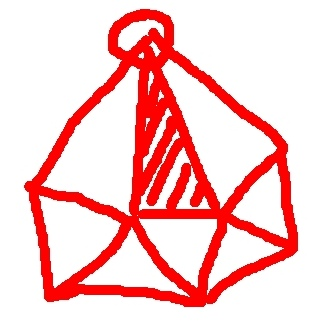
\includegraphics[width=0.2\textwidth]{revision/homotopic_ball.jpg} \quad 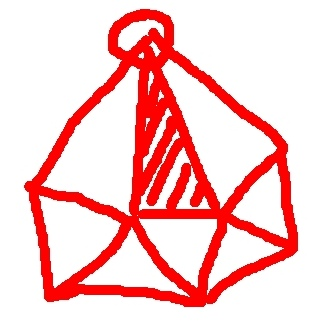
\includegraphics[width=0.2\textwidth]{revision/homotopic_ball.jpg}}
\centering
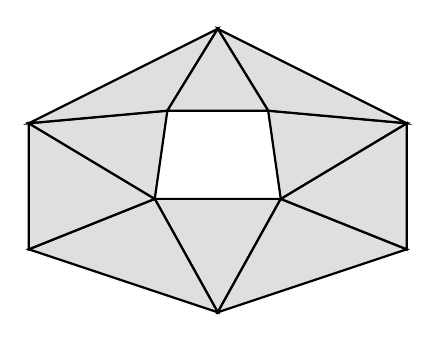
\begin{tikzpicture}[scale=0.8]
    % Coordinates of the main outer triangle
    \coordinate (B0)  at (0,-1); % Bottom left
    \coordinate (BL)  at (-3,0); % Bottom right
    \coordinate (BR)  at (3,0); % Bottom right
    \coordinate (CLL) at (-3,2); % Bottom left
    \coordinate (CL)  at (-1,0.8); % Bottom right
    \coordinate (CR)  at ( 1,0.8); % Bottom right
    \coordinate (CRR) at ( 3,2); % Bottom right
    \coordinate (Z)   at (0,3.5); % Top
    \coordinate (ML) at  (-0.8,2.2);% ($(CL)!0.3!(Z)$);
    \coordinate (MR) at  ( 0.8,2.2);% ($(CR)!0.6!(Z)$);
    \draw[thick,fill=gray!25] (B0) -- (CL) -- (CR) -- cycle;
    \draw[thick,fill=gray!25] (B0) -- (CL) -- (BL) -- cycle;
    \draw[thick,fill=gray!25] (BL) -- (CL) -- (CLL) -- cycle;
    \draw[thick,fill=gray!25] (B0) -- (CR) -- (BR) -- cycle;
    \draw[thick,fill=gray!25] (BR) -- (CR) -- (CRR) -- cycle;
    \draw[thick,fill=gray!25] (ML) -- (CL) -- (CLL) -- cycle;
    \draw[thick,fill=gray!25] (MR) -- (CR) -- (CRR) -- cycle;
    \draw[thick,fill=gray!25] (Z) -- (ML) -- (CLL) -- cycle;
    \draw[thick,fill=gray!25] (Z) -- (MR) -- (CRR) -- cycle;
    \draw[thick,fill=gray!25] (Z) -- (ML) -- (MR) -- cycle;
\end{tikzpicture}
\qquad
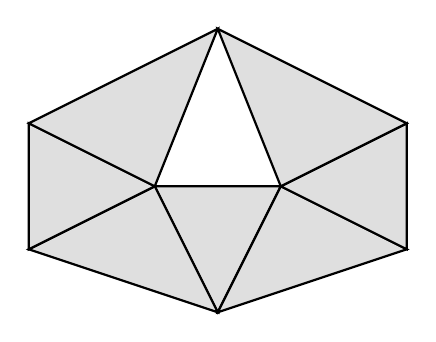
\begin{tikzpicture}[scale=0.8]
    % Coordinates of the main outer triangle
    \coordinate (B0)  at (0,-1); % Bottom left
    \coordinate (BL)  at (-3,0); % Bottom right
    \coordinate (BR)  at (3,0); % Bottom right
    \coordinate (CLL) at (-3,2); % Bottom left
    \coordinate (CL)  at (-1,1); % Bottom right
    \coordinate (CR)  at ( 1,1); % Bottom right
    \coordinate (CRR) at ( 3,2); % Bottom right
    \coordinate (Z)   at (0,3.5); % Top
    \draw[thick,fill=gray!25] (B0) -- (CL) -- (CR) -- cycle;
    \draw[thick,fill=gray!25] (B0) -- (CL) -- (BL) -- cycle;
    \draw[thick,fill=gray!25] (BL) -- (CL) -- (CLL) -- cycle;
    \draw[thick,fill=gray!25] (B0) -- (CR) -- (BR) -- cycle;
    \draw[thick,fill=gray!25] (BR) -- (CR) -- (CRR) -- cycle;
    \draw[thick,fill=gray!25] (Z) -- (CL) -- (CLL) -- cycle;
    \draw[thick,fill=gray!25] (Z) -- (CR) -- (CRR) -- cycle;
\end{tikzpicture}

\caption{Left: manifold triangulation of an annulus. Right: not a manifold triangulation.}
\label{figure:not_manifold_triang}
\end{figure}


\subsection{Triangulations of manifolds}\label{subsection:manifoldtriangulation}

Our discussion requires some notions and results concerning triangulated manifolds. 
We define an $n$-dimensional simplicial complex to be a \emph{manifold triangulation} if the underlying set $\underlying{\calT}$ is an $n$-dimensional manifold with boundary.
We recall that this means that for every $x \in \underlying{\calT}$
% there exists $\epsilon > 0$ and an embedding $\phi : \Ball_\epsilon(x) \cap \underlying{\calT} \rightarrow \bbR^{n}$
there exists an open neighborhood $U(x) \subseteq \underlying{\calT}$ and an embedding $\phi : U(x) \rightarrow \bbR^{n}$
such that $\phi(0) = 0$ and $\phi$ is an isomorphism either onto the open unit ball $\calB = \{ x \in \bbR^{n} \suchthat |x| < 1 \}$
or onto the half-ball $\{ x \in \calB \suchthat x_1 \geq 0 \}$.
In the former case, $x$ is called an \emph{interior point}, and in the latter case $x$ is called a \emph{boundary point}. 
Any simplicial complex that triangulates an $n$-dimensional manifold must be $n$-dimensional. 
An example of a manifold triangulation and an example which is not a manifold triangulation are given in Figure~\ref{figure:not_manifold_triang}.

The following special cases receive particular interest:
an \textit{$n$-ball triangulation} is any triangulation of a topological (closed) $n$-ball, and we sometimes call this an \textit{$n$-disk} triangulation.
An \textit{$n$-sphere triangulation} is any triangulation of a topological $n$-sphere. 


We know that any manifold $\calM$ has got a topological boundary $\partial\calM$, possibly empty. 
If $\calM$ is $n$-dimensional, then the $\partial\calM$ is a topological manifold without boundary of dimension $n-1$. 
We gather a few helpful observations on how these notions relate to triangulations.
While the reader might deem them obvious, we nevertheless include proofs. 

\begin{lemma}\label{lemma:boundarysimplices}
    Let $\calT$ be a finite $n$-dimensional simplicial complex whose underlying set is a manifold $\calM$. 
    Then the simplices contained in the boundary constitute a triangulation of the boundary.
    Moreover, if $F \in \calT$ is a face (i.e, $F$ has dimension $n-1$), then 
    \begin{itemize}
        \item $F$ is not contained in the boundary if and only if it is contained in exactly two $n$-simplices.
        \item $F$ is contained in the boundary if and only if it is contained in exactly one $n$-simplex.
        % \item $\calT$ is non-branching, that is, every $F \in \calT$ of dimension $n-1$ is contained in at most two $n$-simplices of $\calT$. 
    \end{itemize}
\end{lemma}
\begin{proof}
    We prove these statements in several steps.
    \begin{enumerate}
    \item 
    Let $\mathring \calM := \calM \setminus \partial \calM$ denote the interior of the manifold. 
    We will use the following fact:\footnote{To see this, one easily constructs a continuous deformation of $\calM$ into itself to move any chosen point on $S$ to any other chosen point on $S$.} if $S \in \calT$ has an inner point that lies on $\partial \calM$, then all inner points of $S$ are on $\partial \calM$. 
    Since the boundary $\partial \calM$ is closed, every $S \in \calT$ is either a subset of the boundary or all its inner points lie in the interior $\mathring \calM$ of the manifold. 
    
    \item 
    We recall an auxiliary result.
    Suppose that $Y$ is a topological space homeomorphic to a sphere of dimension $m$ and that $X \subseteq Y$ is homeomorphic to a sphere of dimension $m-1$, where $m \geq 1$. 
    As a consequence of the Jordan--Brouwer separation theorem~\cite[Corollary IV.5.24]{mayer1989algebraische}~\cite[Corollary VIII.6.4]{massey1981algebraic}, 
    we know that $Y \setminus X$ has got two connected components.
    
    % \item 
    % We prove an auxiliary result. 
    % Suppose that $Y$ is a topological space homeomorphic to a sphere of dimension $m$ and that $X \subseteq Y$ is homeomorphic to a sphere of dimension $m-1$, where $m \geq 1$. 
    % The embedding of $X$ into $Y$ cannot be onto~\cite[Theorem~2.55]{lee2011topological}, and so there exists $y \in Y \setminus X$. 
    % Using the homeomorphism from $Y$ into the $m$-sphere, which maps $y$ to the north pole without loss of generality, and a stereographic projection, 
    % we see that $Y \setminus \{y\}$ is homeomorphic to $R^{m}$.
    % As a consequence of the Jordan--Brouwer separation theorem~\cite[Theorem IV.5.23]{mayer1989algebraische}~\cite[Corollary IV.5.24]{mayer1989algebraische}~\cite[Corollary VIII.6.4]{massey1981algebraic}, $Y \setminus (X \cup \{y\})$ has got two connected components,
    % and thus $Y \setminus X$ has got two connected components.
    
    \item
    Let now $F \in \subsimplex_{n-1}(T)$ be a face and let $z_F \in F$ be its barycenter. 
    Since $\calT$ is finite, we let $\mathring B_F$ be an open neighborhood around $z_F$ 
    homeomorphic to an $n$-dimensional ball 
    so small that its closure $\overline{B_F}$ only intersects those $n$-simplices of $\calT$ that already contain $z_F$ and no faces other than $F$.
    Suppose there are distinct $n$-simplices $T_1, T_2, \dots, T_K$ that contain $z_F$. 
    The intersection of any two of them is $F$, but their interiors are disjoint because otherwise they would coincide. 
    
    If $z_F$ is an interior point of $\calM$, 
    then it follows by our assumptions that $\mathring B_F$ is homeomorphic to an open $n$-ball and $\partial \mathring B_F$ is homeomorphic to a sphere of dimension $n-1$. 
    Consider $X = F \cap \partial \mathring B_F$.
    If $n=1$, then $X$ is empty and $\partial \mathring B_F$ has $K$ distinct connected components. 
    If $n > 1$, then $X$ is homeomorphic to a sphere of dimension $n-2$
    and again $\partial \mathring B_F \setminus X$ has $K$ distinct connected components. 
    But by the auxiliary result above, $K = 2$. 
    We conclude that $F$ is contained in two $n$-simplices of $\calT$.
    
    Consider the case that $z_F$ lies on the boundary of $\calM$ and suppose that $F$ is contained in $K$ distinct $n$-simplices of $\calT$.
    By adding at least one dimension, we can double\footnote{The reader is referred to Lee's textbook~\cite{lee2012smooth} for more background and the technicalities.} the manifold $\calM$ along the boundary and obtain the doubled manifold $\calM'$. 
    Similarly, we can construct a doubling of the triangulation $\calT'$ such that $F$ is contained in exactly $2K$ distinct $n$-simplices of $\calT'$. 
    We know that $\calM'$ is a manifold without boundary, and hence $F$ is an interior simplex of $\calT'$.
    This implies $K=1$.
    So any boundary face can only be contained in one single $n$-simplex. 
    
    \item
    Clearly, the simplices of $\calT$ contained in the boundary constitute a simplicial complex. 
    Every $x \in \calM$ is an inner point of some simplex $S \in \calT$. 
    If $x \in \partial \calM$ is a boundary point, then $S$ must be a boundary simplex, 
    so the boundary simplices triangulate all of $\partial \calM$.
    \end{enumerate}
    All desired results are thus proven. 
\end{proof}

Suppose that $\calT$ is an $n$-dimensional simplicial complex that triangulates a manifold. 
Those simplices of the manifold triangulation that are subsets of the boundary of the underlying manifold are called \emph{boundary simplices}. 
% The simplices that lie in the boundary of the underlying set are called \emph{boundary simplices}.
All other simplices of the manifold triangulation are called \emph{inner simplices}. 
We have seen that the boundary simplices of a manifold triangulation constitute a triangulation of the manifolds boundary. 
We call this simplicial complex the \emph{boundary complex}. It has dimension $n-1$. 
% We see that the family of boundary faces constitute a simplicial complex, which we call \textit{boundary complex}.
% Any point on the boundary lies within some boundary simplex, and hence the boundary complex is a triangulation of the boundary. 
% Definitions imply that the boundary complex is a manifold triangulation of dimension $n-1$.
% The boundary simplices of a manifold triangulation of dimension $n$ constitute a manifold triangulation themselves, of dimension $n-1$, which triangulate the boundary of the underlying space. 

We continue with a few more observations about the topology of local patches (stars) of manifold triangulations. This topics is surprisingly non-trivial and 
we gather some results that are hard to find in the literature. 

\begin{lemma}\label{lemma:startopology}
    Let $\calT$ be a finite $n$-dimensional simplicial complex whose underlying space is a manifold $\calM$.
    Suppose that $1 \leq n \leq 3$. Then the following holds:
    \begin{itemize}
        \item
        If $S \in \calT$ is an inner simplex, 
        then $\patch_{\calT}(S)$ is a simplicial $n$-ball with $S$ as an inner simplex
        and $\carapace_{\calT}(S)$ is a simplicial $(n-1)$-sphere. 
        \item
        If $S \in \calT$ is a boundary subsimplex, 
        then $\patch_{\calT}(S)$ is a simplicial $n$-ball with $S$ as a boundary simplex,
        and $\carapace_{\calT}(S)$ is a simplicial $(n-1)$-ball.
    \end{itemize}
\end{lemma}
\begin{proof}
    The lemma is obvious if $n = 1$, so we assume $n \geq 2$ in what follows. 
    We prove these statements in several steps. 
    The reader is assumed to have some background in topology. 
    \begin{enumerate}
    \item 
    Let $S$ be any simplex with vertices $v_0, v_1, \dots, v_k$, with barycenter $z_{S}$, and dimension $k$.
    Let $\calS := \patch_{\calT}(S)$ be its star. 
    Each $l$-dimensional simplex $T \in \calS$ that contains $S$ 
    has vertices $v_0$, $v_1$, $\dots$, $v_k$, $v_{k+1}^{S}$, $\dots$, $v_{l}^{S}$. 
    For any such simplex, we introduce a decomposition $T_{0}, \dots, T_{k}$, where each $T_{i}$ has vertices 
    $v_0$, $\dots$, $v_{i-1}$, $z_{S}$, $v_{i+1}$, $\dots$, $v_k$, $v_{k+1}^{S}$, $\dots$, $v_{l}^{S}$.
    % \begin{align*}
        % v_0, \dots, v_{i-1}, z_{S}, v_{i+1}, \dots, v_k, v_{k+1}^{S}, \dots, v_{l}^{S}. 
    % \end{align*}
    The collection $\calS'$ of these simplices and their subsimplices constitute a simplicial complex 
    that triangulates the same underlying set as $\calS$.
    Moreover, $\calS' = \patch_{\calS'}(z_{S})$. 
    In particular, $z_{S}$ is a boundary vertex of $\calS'$ if and only if $S$ is a boundary simplex of $\calS$. 
    So it remains to study the topology of vertex stars. 
    
    \item 
    Suppose that $2 \leq n \leq 3$ and that $\calM$ is a manifold without boundary. 
    Under these assumptions, 
    as explained in the proof of Theorem~1 in \cite{Siebenmann1979},
    the set $\carapace(V)$ is a triangulation of a sphere of dimension $n-1$ for any inner vertex $V$. 
    There exists a homeomorphism from the closed cone of $\underlying{\carapace(V)}$ onto the local star $\underlying{\patch_{\calT}(V)}$.
    But then that closed cone and hence $\underlying{\patch_{\calT}(V)}$ are homeomorphic to an $n$-dimensional ball. 
    
    \item 
    If $2 \leq n \leq 3$ and $\calM$ has a non-empty boundary, then we use an approach as in the proof of Lemma~\ref{lemma:boundarysimplices}: 
    we let $\calM'$ denote the doubling of the manifold and $\calT'$ be the doubling of the triangulation $\calT$. 
    Let $V \in \calT$ be a vertex. 
    If $V$ is an inner vertex of $\calT$, then $\carapace(V) \subseteq \calT \subseteq \calT'$ triangulates a sphere of dimension $n-1$ and $\patch_{\calT}(V) \subseteq \calT \subseteq \calT'$ triangulates a ball of dimension $n$, as discussed above. 
    If $V$ is a boundary vertex of $\calT$, then it is an inner vertex of $\calT'$,
    and so $\carapace_{\calT}(V) \subseteq \calT'$ triangulates a sphere of dimension $n-1$ and $\patch_{\calT}(V) \subseteq \calT'$ triangulates a ball of dimension $n$.
    We also know that $\carapace_{\partial\calT}(V) \subseteq \partial\calT$ triangulates a sphere of dimension $n-2$ and $\patch_{\partial\calT}(V) \subseteq \partial\calT$ triangulates a ball of dimension $n-1$. 
    The embedding of $\carapace_{\partial\calT}(V) \subseteq \partial\calT$ is homeomorphic to the standard embedding of the $(n-2)$-dimensional unit sphere into the $(n-1)$-dimensional unit sphere,
    by the topological Schoenflies theorem. 
    It follows that $\carapace_{\calT}(V)$ triangulates a topological ball of dimension $n-1$.
    Since the closed cone of $\underlying{\carapace(V)}$ is homeomorphic to the star $\underlying{\patch_{\calT}(V)}$, we conclude that $\patch_{\calT}(V)$ triangulates an $n$-dimensional ball. 
    
    
%     Suppose that $S = \{z\}$ is a singleton simplex. 
%     For $\delta > 0$ small enough, 
%     \begin{align*}
%         B_{\delta}(z) = \left\{ x \in \calM \suchthat d(x,z) \leq \delta \right\},
%         \quad 
%         S_{\delta}(z) = \left\{ x \in \calM \suchthat d(x,z) = \delta \right\},
%     \end{align*}
%     are compactly contained subsets of $|\patch_{\calT}(S)|$.
%     For each simplex $K \in \patch_{\calT}(S)$ that contains the vertex $z$ and which has the opposite face $F_K$, 
%     we easily find homeomorphisms $\phi_{K} : B_{\delta}(z) \cap K \rightarrow K$
%     such that 
%     $\phi_{K}(z) = z$, 
%     such that 
%     $\phi_{K}( K \cap S_{\delta}(z) ) = F_{K}$,
%     such that 
%     for all $K, K' \in \calT$ with $K' \subseteq K$ we have $\phi_{K|K'} = \phi_{K'}$,
%     and such that 
%     $\phi_{K}$ maps $[0,1]\cdot v$ linearly into $\bbR \cdot v$. 
%     This is defines a homeomorphism $\phi : B_{\delta}(z) \rightarrow |\patch_{\calT}(S)|$. 
%     Moreover, one easily verifies that $\phi$ is bi-Lipschitz.
%     %     For $\delta > 0$ small enough, $B_{\delta}(z)$ is homeomorphic to the unit ball and that homeomorphism maps $S_{\delta}(z)$ onto the unit sphere. 
%     \item 
%     One sees that $\phi$ defines a mapping from the closed 
%     homeomorphism between cone of link and ball 
%     
%     If $z$ is an inner vertex of $\calS'$, 
%     then the boundary simplices of $\calS'$,
%     which are the boundary simplices of $\calS$, triangulate a topological sphere of dimension $n-1$.
%     
%     Now suppose that $z$ is a boundary vertex of $\calS'$,
%     which is the case if and only if $S$ is a boundary simplex. 
%     Write 
%     \[
%         B_{H} = \left\{ x \in B_1(0) \suchthat* x_1 \leq 0 \right\},
%         \quad 
%         S_{H} = \left\{ x \in \partial B_1(0) \suchthat* x_1 \leq 0 \right\}.
%         \quad 
%         D_{H} = \left\{ x \in \partial B_1(0) \suchthat* x_1 = 0 \right\}.
%     \]
%     Provided that $\delta > 0$ is small enough, there exists a homeomorphism $\phi'$ that maps $\overline{B_{\delta}(z)} \cap \calM$ onto $B_1(0)$, which maps $\overline{B_{\delta}(z)} \cap \partial\calM$ onto $D_H$,
%     and which maps $z$ to the origin. 
%         %
%     It follows that $\phi'$ maps the closure of $\partial{B_{\delta}(z)} \setminus \partial\calM$ onto $S_H$.
%         %
%     Assuming that $\delta$ is small enough once more, 
%     we now verify that $\phi^{-1}$ maps $|\carapace(S)|$ onto $S_{\delta}(z) \cap |\patch_{\calT}(S)|$.
%     The latter equals the closure of $\partial{B_{\delta}(z)} \setminus \partial\calM$.
%     It follows that $\carapace(S)$ triangulates a topological ball of dimension $n-1$. 
    % We let $\calM'$ be the doubling of the manifold and let $\calT'$ be the doubling of the present triangulation;
    % we refer to Lee's textbook~\cite{lee2011topological} for details. 
    % The vertex star around $z$ within the boundary triangulation $\partial\calT$ is homeomorphic to the ball of dimension $n-1$,
    % and it is homeomorphic to $\overline{ B_{\delta}(z) } \cap |\partial\patch_{\calT}(S)|$ along $\phi$. 
    % The underlying space of $\carapace(S)$ is homeomorphic to $S_{\delta}(z) \cap |\patch_{\calT}(S)|$ along $\phi$.
    % The vertex star around $z$ within the boundary triangulation $\partial\calT$ is homeomorphic to the ball of dimension $n-1$,
    % and it is homeomorphic to $\overline{ B_{\delta}(z) } \cap |\partial\patch_{\calT}(S)|$ along $\phi$. 
    % Notice that 
    % \begin{align*}
    %     \partial\left( { B_{\delta}(z) } \cap |\partial\patch_{\calT}(S)| \right)
    %     =
    %     S_{\delta}(z) \cap |\patch_{\calT}(S)|
    %     \cup 
    %     \overline{ B_{\delta}(z) } \cap |\partial\patch_{\calT}(S)|
    %     .
    % \end{align*}
    % Necessarily, this homeomorphism maps the boundary of $\overline{B_{\delta}(z)} \cap \underlying{\calT}$, which contains $z$, onto the unit sphere. Since the image of $\overline{ B_{\delta}(z) } \cap |\partial\patch_{\calT}(S)|$ along $\phi'$ is still homeomorphic to a disk of dimension $n-1$, so must be the image of $S_{\delta}(z) \cap |\patch_{\calT}(S)|$ under $\phi'$.
    % But that just means that $\carapace(S)$ triangulates a topological ball of dimension $n-1$. 
    \end{enumerate}
    All relevant results are proven. 
\end{proof}


\begin{lemma}\label{lemma:connectivity}
    Let $\calT$ be a finite $n$-dimensional simplicial complex whose underlying space is a manifold $\calM$.
    If the underlying space of $\calT$ is connected, then $\calT$ is face-connected.
\end{lemma}
\begin{proof}
    We first show that each vertex star is face-connected via a short induction argument.
    Clearly, any simplicial $1$-ball and simplicial $1$-sphere are face-connected. 
    Now, if $n \geq 1$, then any vertex star in any $(n+1)$-dimensional manifold triangulation is already face-connected if all simplicial $n$-balls and $n$-spheres are face-connected.
    The induction argument implies that each vertex star in $\calT$ is face-connected.

    If the underlying space $\underlying{\calT}$ is connected, 
    then we easily see that the union of the $1$-simplices is path-connected.
    Given $n$-simplices $S,S' \in \calT$, 
    we can thus choose a sequence of $\hat S_0=S,\hat S_1,\dots,\hat S_m=S' \in \calT$ such that $\hat S_{i} \cap \hat S_{i-1} \neq \emptyset$ for all $1 \leq i \leq m$, and so each two consecutive simplices in that sequence have at least one vertex in common. 
    As each vertex star is face-connected, 
    we can thus assume without loss of generality that the sequence $S_0=S,S_1,\dots,S'=S_m \in \calT$ 
    is such that $S_{i} \cap S_{i-1}$ is a face of both $S_{i}$ and $S_{i-1}$ for all $1 \leq i \leq m$.
    This just means that $\calT$ is face-connected. 
\end{proof}



\begin{remark}
    Triangulations with the property that all vertex stars are homeomorphic to a ball are also called \emph{combinatorial} \cite[Section~1]{Bagchi2005}.
    All manifolds of dimension up to three admit smooth structures and smooth manifolds admit combinatorial triangulations. 
    There are triangulations of manifolds in more than three dimensions where not every vertex star is homeomorphic to a ball. 
    
    Not every simplicial complex is the triangulation of some (embedded) topological manifold with or without boundary. 
    When the dimension is at least five, then there is no computer algorithm that, given a finite simplicial complex as input, decides whether the input is the triangulation of some fixed manifold~\cite{chernavsky2006unrecognizability}.
    Going further, it has been shown that deciding whether a simplicial complex is the triangulation of a manifold cannot be decided by any computer algorithm~\cite{poonen2014undecidable}.     
    % Whether a simplicial complex is the triangulation of a manifold is algorithmically undecidable. ~\cite{todo}
    We therefore are not in pursuit of any easy combinatorial property that indicates whether a simplicial complex (without any further specific assumptions) triangulates a manifold.

    Conversely, not all topological manifolds, even if compact, can be described as a triangulation. 
    Such manifolds, some even compact and simply-connected, appear in dimension four and higher~\cite{akbulut2014casson}.
%     For each dimension $n \geq 5$ there exists an $n$-dimensional compact topological manifold without a triangulation. 
\end{remark}








% 3. Shellability 
\subsection{Shellable simplicial complexes}\label{subsection:shellability}


The notions of shelling and shellable triangulation have been discussed widely in combinatorial topology and polytopal theory. 
Formally, a triangulation is shellable if its full-dimensional simplices can be enumerated such that each simplex intersects the union of the previously listed simplices in a codimension one triangulation of a manifold. 
This forces the intermediate triangulations to be particularly well-shaped. 
We build upon the notion of shelling as introduced in~\cite[Definition 8.1]{ziegler1995lectures},
where our definition of shelling is equivalent to the notion of the shellings of simplicial complexes, see also~\cite[Remark~8.3]{ziegler1995lectures}. 

% \mwl{Roughly speaking, a triangulation is shellable if the triangulation can be built, starting from a single simplex,
% by successively gluing simplices to intermediate triangulations such that a combinatorial-geometric condition is satisfied:
% the gluing interface is a triangulated submanifold of the boundary. 
% This forces the intermediate triangulations to be particularly well-shaped. 
% We turn our attention to a different idea of how to incrementally construct a simplicial complex while maintaining well-behaved intermediate complexes. 
%It is often very helpful if a simplicial complex can be created recursively, starting with a single simplex, as this enables the inductive method of proof.
% }



Suppose that $\calT$ is an $n$-dimensional simplicial complex and we have an enumeration of the $n$-simplices $T_{0}, T_{1}, T_{2}, \dots \in \subsimplex_{n}(\calT)$.
For any enumeration, we call 
\begin{align*}
    \Gamma_m 
    := 
    \big( 
        T_{0} \cup T_{1} \cup \dots \cup T_{m} 
    \big) 
    \cap 
    T_{m+1}
\end{align*}
the $m$-th \textit{interface set}. 
% Note that this intersection is automatically a subcomplex of the boundary complex of the last simplex $T_{m}$.
We call the enumeration a \emph{shelling} if each interface set $\Gamma_m$ is a triangulated manifold of dimension $n-1$. 

The reason of our interest in shellable simplicial complexes is that they can be constructed via successive adhesion of simplices.
The resulting succession of simplicial complexes consists of simplicial balls or spheres. 

\begin{lemma}\label{lemma:shell_triang_man}
    Let $\calT$ be an $n$-dimensional simplicial complex 
    with a shelling $T_{0}, T_{1}, T_{2}, \dots, T_{M}$,
    such that each simplex of dimension $n-1$ is contained in at most two simplices. 
    % DONE: what is non-branching?
    Then
    $$
        X_{m} := T_{0} \cup T_{1} \cup \dots \cup T_{m}
    $$ 
    is a triangulated manifold with boundary for all $0 \leq m \leq M$.
    % 
    In particular, $X_{m}$ is a topological $n$-ball when $m < M$, 
    and 
    $X_{M}$ is either a topological $n$-ball or topological $n$-sphere. 
\end{lemma}
\begin{proof}  
    We prove this claim by induction. 
    Certainly, if $\calT$ contains only one single $n$-simplex, then it is a shellable triangulation of a topological $n$-ball. Let $1 \leq m \leq M$ and suppose that 
    \begin{align*}
        X_{m-1} := T_{0} \cup T_{1} \cup \dots \cup T_{m-1}
    \end{align*}
    is a topological $n$-ball. Let $T_{m}$ is the next $n$-simplex in the shelling.
    By definition, $\Gamma_{m} := X_{m-1} \cap T_{m}$ is a submanifold of $\partial T_{m}$,
    and it is triangulated by some faces of $T_{m}$ and their subsimplices. 
    
    Let $F$ be such a face. 
    By assumption, $F$ must be contained in exactly one $n$-simplex of $T_{0}, T_{1}, \dots, T_{m-1}$,
    and $F$ is in the boundary of $X_{m-1}$. 
    We conclude that $\Gamma_{m}$ triangulates a submanifold of the boundary of $X_{m-1}$.
    
    On the one hand, 
    if $\Gamma_{m}$ is the entire boundary of $T_{m}$, 
    then it must also be the boundary of the topological $n$-ball $X_{m-1}$. 
    Hence $X_{m-1} \cup T_{m}$ must be a topological $n$-sphere and thus a manifold without boundary, 
    which requires $m = M$.
    On the other hand, 
    if $\Gamma_{m}$ is a proper subset of the entire boundary of $T_{m}$, 
    then $X_{m-1} \cup T_{m}$ is still a topological $n$-ball.
\end{proof}


\begin{remark}
    We interpret a shelling as the construction of a triangulation 
    by successively attaching simplices such that the intermediate triangulations are well-behaved. 
    Conversely, the reverse enumeration describes a successive decomposition of the triangulation, hence the name ``shelling''.
\end{remark}
\begin{remark}
    Whether a simplicial complex is shellable can be checked, in principle, simply by trying out all the possible enumerations.
    That we cannot do much better than this is captured in the result that testing for shellability is NP-complete~\cite{goaoc2019shellability}:
    this complexity result is even true if we merely consider simplicial complexes of dimension two embedded in some Euclidean space.
\end{remark}

We now collect important examples of shellable triangulations. Essentially, in two space dimensions, interesting triangulations are shellable, but starting from three space dimensions, non-shellable situations can arise. Our main interest are local patches (stars) within triangulations: these are shellable up to three space dimensions, but not necessarily beyond. 

\begin{example}\label{example:shell_simpl}
    Any simplex $T$ (trivially) has a shelling, consisting only of $T$ itself. 
    The boundary complex $\partial \calT(T)$ has a shelling:
    any enumeration of the boundary faces of $T$ constitutes a shelling; see Example 8.2.(iii) in~\cite{ziegler1995lectures}.
\end{example}
\begin{example}
    The standard triangulation of the $3$-dimensional cube by six tetrahedra, the Kuhn triangulation~\cite{kuhn1960some}, is shellable, as are its higher-dimensional generalizations.\footnote{We remark that Kuhn attributes this triangulation to Lefschetz~\cite{lefschetz2015introduction}.}
\end{example}
\begin{example}
    There exists a non-shellable triangulation of a tetrahedron and of a cube in $n=3$, see~\cite[Example 8.9]{ziegler1995lectures}.
\end{example}

\begin{lemma}\label{lemma:shell_2D}
    Any simplicial $2$-\disk\ is shellable.
    Any simplicial $2$-sphere is shellable. 
\end{lemma}
\begin{proof}
    First, 
    let $\calS$ be any triangulation of a $2$-sphere. 
    By removing any triangle $S \in \calS$, we obtain a triangulation $\calT$ of a $2$-\disk.
    Any shelling of that \disk\ can be extended to a shelling of $\calS$ by re-inserting the first triangle $S$.
    So it remains to show that any triangulation $\calT$ of the two-dimensional \disk\ is shellable. 
    We will construct the shelling in reverse. 
    
    Write $M = \underlying{\calT}$. 
    There is nothing to show if $\calT$ contains only one triangle. 
    We call a triangle $T \in \calT$ \emph{good in $\calT$} if it intersects the boundary $\partial M$ in a non-empty union of edges. 
    Hence a triangle is good in $\calT$ if its intersection with $\partial M$ is either one, two, or three edges,
    and a triangle is not good in $\calT$ if that intersection is either empty, only some of its vertices, or a vertex and the opposite edge.
    % DONE: I understand what it means from the rest of the proof, but I believe it could a bit more explicit.
    We show by an induction argument over the number of triangles that every triangulation of a $2$-\disk\ that contains at least two triangles also contains at least two good triangles. 

    Clearly, this is the case if the triangulation of the $2$-\disk\ contains two triangles. 
    Now suppose the induction claim is true when the triangulation includes at most $N$ triangles,
    and assume that $\calT$ includes $N+1$ triangles. 
    As we travel along the boundary, we traverse along edges of at least two simplices, 
    and therefore there are at least two triangles with an edge on the boundary. 
    Suppose that $\calT$ does not have at least two triangles that are good in $\calT$.
    Then there exists a triangle $T'$ that intersects $\partial M$ 
    in one edge and its opposite vertex.
    Removing $T'$ splits the manifold into two face-connected components, each of which is a topological $2$-\disk. 
    By the induction assumption, each of those components contains at least two triangles 
    that are good in the respective component. 
    So each component has at least one triangle that is also good in $\calT$. 
    Hence $\calT$ contains two good triangles, which completes the induction step. 
    
    We conclude that whenever $\calT$ triangulates a $2$-\disk,
    it contains a good triangle $T$. 
    If $T$ has three edges in the boundary, then $T = M$ and we are trivially done. 
    If $T$ intersects with the boundary in exactly one or two edges, 
    then $\overline{M \setminus T}$ is still a topological $2$-\disk.
    The triangulation $\calT'$ that is obtained by removing $T$
    is a triangulation of some $2$-\disk\ that intersects $T$ only at either two or one edges.
    Any shelling of $\calT'$ can in this way be extended to a shelling of $\calT$, and the proof is complete. 
\end{proof}

\begin{lemma}
    Let $\calT$ be a $3$-dimensional manifold triangulation and $S \in \calT$.
    Then $\patch_{\calT}(S)$ is shellable. 
\end{lemma}
\begin{proof}
    The statement is trivially true if $S$ is a tetrahedron. 
    The statement is clear if $S$ is an inner or boundary face of $\calT$,
    where we only need to enumerate either one or two tetrahedra. 
    The statement is still easily verified if $S$ is an inner or boundary edge of $\calT$:
    one chooses a starting tetrahedron (with a boundary face if $S$ is a boundary edge) and rotates around the edge in a fixed direction to create a suitable enumeration. 
    When $S$ is an inner vertex, then the faces (triangles) of $\patch_{\calT}(S)$ that do not contain $V$ constitute a simplicial $2$-sphere.
    Similarly, when $S$ is a boundary vertex, then the faces (triangles) of $\patch_{\calT}(S)$ that do not contain $V$ constitute a simplicial $2$-\disk.
    Both these $2$-dimensional complexes are shellable by Lemma~\ref{lemma:shell_2D}, and any such shelling immediately yields a shelling of $\patch_{\calT}(S)$ since there is a one-to-one correspondence between the tetrahedra in $\calT$ and the triangles.
    \footnote{For $S$ an inner vertex, \cite[Lemma~B.1]{ern2020stable} also yields the claim.}
\end{proof}


\begin{lemma}\label{lemma:stars_are_shellable}
    Let $\calT$ be a $n$-dimensional shellable triangulation and $V \in \Vertices(\calT)$ be a vertex.
    Then $\patch_{\calT}(V)$ is shellable. 
\end{lemma}
\begin{proof}
    This is Lemma~8.7 in \cite{ziegler1995lectures}.
%     Without loss of generality, $V$ is the origin. 
%     Any ray starting at $V$ intersects at most one vertex of $\patch_{\calT}(V)$.
%     We can also assume that all boundary vertices of $\patch_{\calT}(V)$ to be unit vectors,
%     which does not affect shellability. 
%     The simplicial boundary complex of $\calT$ is the boundary complex of a convex polytope,
%     and is thus shellable~\cite[Theorem~8.12]{ziegler1995lectures}. 
\end{proof}


\begin{remark}
    Not all triangulable sets admit a triangulation that is shellable. 
    Moreover, even if a set admits a shellable triangulation, not all of its triangulations are shellable. For example, if we extend the non-shellable triangulation of the tetrahedron from~\cite[Example 8.9]{ziegler1995lectures} to a triangulation of a hypertetrahedron by suspending it from a new point $v_\star$, then the resulting new triangulation is non-shellable and coincides with the patch around $v_\star$.
    This demonstrates that patches around boundary simplices are not necessarily shellable when the space dimension $n$ is larger than three.
\end{remark}
\begin{remark}
    Not all triangulable sets admit a triangulation that is also shellable. 
    Moreover, even if a set admits a shellable triangulation, not all of its triangulations might be shellable. 
    We refer to~\cite[Example 8.9]{ziegler1995lectures} for an examples of non-shellable triangulations of cubes and tetrahedra in three dimensions. 
\end{remark}


A major structural feature of shellable simplicial complexes is that each time an $n$-simplex is added, stars around lower-dimensional simplices gets completed. 

\begin{lemma}\label{lemma:existenceofstar}
    Suppose that an $n$-dimensional manifold triangulation $\calT$ has a shelling $T_{0}, T_{1}, T_{2}, \dots, T_{M}$.
    For $0 \leq m \leq M$, write 
    $$
        X_{m} := T_{0} \cup T_{1} \cup \dots \cup T_{m}.
    $$ 
    For $1 \leq m \leq M$, write 
    $$
        \Gamma_{m} := X_{m-1} \cap T_{m}.
    $$ 
    Then $\Gamma_{m}$ is a union of $\ell$ different faces of $T_{m}$, $1 \leq \ell \leq n+1$.
    If $m < M$, then the intersection of those faces is an interior simplex $S_{m} \in \calT$ of dimension $n-\ell$ that satisfies 
    $$
        \patch_{X_{m}}(S_{m}) = \patch_{\calT}(S_{m}).
    $$
\end{lemma}
\begin{proof}
    We know $\Gamma_{m}$ is a triangulated submanifold of the boundary of $T_{m}$, 
    and so it must be a collection of $\ell$ faces of $T$, $1 \leq \ell \leq n+1$.
    Note that $\ell = n + 1$ can only happen for the last enumerated simplex, $m = M$, if $\calT$ triangulates an $n$-sphere. 
    $\Gamma_{m}$ also constitutes a local patch (star) of $(n-1)$-dimensional simplices around some simplex $S_{m}$ of dimension $n-\ell$ in $\Gamma_{m}$.
    By definition, $S_{m}$ is a boundary simplex of $X_{m}$, 
    and it is an interior simplex of $X_{m+1}$. 
    But then $S_{m}$ cannot be a subsimplex of any of the simplices $T_{m+1}, \dots, T_{M}$,
    which means that $\patch_{X_{m+1}}(S_{m}) = \patch_{\calT}(S_{m})$. 
\end{proof}











 




















 
 
 
 
 
 
 
 
 
 
 
 
 
 
 
 
 
 
 
 
 
 
 
 
\section{Reflections and Deformations on shellable stars}\label{section:extension}

This section is devoted to geometric operations that are crucial for our main result in Section~\ref{section:poincarefriedrichs} below. 
Consider the situation where we have an $n$-dimensional local patch (star) around some simplex $S$ and some $n$-dimensional simplex $T$ within that local star. 
We construct a homeomorphism going from the simplex $T$ onto its complement within the local star around $S$,
similar to the two- and three-color maps in \cite[Sections~5.3 and~6.3]{ern2020stable} and the symmetrization maps in~\cite[Section~7.6]{Chaum_Voh_p_rob_3D_H_curl_24}
This homeomorphism, which we interpret as a nonlinear reflection, is required to preserve the interface. 
We ensure that the homeomorphism is bi-Lipschitz, and we are particularly interested in the norms of its Jacobian.
This nonlinear reflection will be used subsequently in generalizing the discussion in Section~\ref{section:gradient} to the setting of differential forms. 
Additionally, this endeavor produces another geometric tool:
we construct a bi-Lipschitz deformation which contracts the entire star into the complement of the newly completed star. 
This deformation will enable additional estimates of Poincar\'e--Friedrichs constants. 



% \begin{figure}
% \tdplotsetmaincoords{60}{120}
% \centering
% \begin{tikzpicture}[tdplot_main_coords]
% \coordinate (A) at (0, 0, 0);
% \coordinate (B) at (2, 0, 0);
% \coordinate (C) at (1, 1.73, 0); % 1.73 = sqrt(3) for an equilateral triangle
% \coordinate (D) at (1, 0.58, 1.63); % 1.63 = sqrt(8/3) for a regular tetrahedron
% \coordinate (A) at (0, 0, 0);
% \coordinate (B) at (2, 0, 0);
% \coordinate (C) at (1, 1.73, 0); % 1.73 = sqrt(3) for an equilateral triangle
% \coordinate (D) at (1, 0.58, 1.63); % 1.63 = sqrt(8/3) for a regular tetrahedron
% \draw[thick] (A) -- (B) 
% \draw[] (B) -- (C) 
% \draw[] (C) -- (A) 
% \draw[] (A) -- (D);
% \draw[thick] (B) -- (D);
% \draw[] (C) -- (D);
% \node at (A) [below left] {$A(0,0,0)$};
% \node at (B) [below right] {$B(2,0,0)$};
% \node at (C) [above right] {$C(1,\sqrt{3},0)$};
% \node at (D) [above] {$D(1, \frac{1}{\sqrt{3}}, \sqrt{\frac{8}{3}})$};
% \end{tikzpicture} 
% \caption{test}
% \end{figure}



We will use the following observation, which we state without proof, 
that controls the volume and some heights when a simplex is partitioned via barycentric subdivision.

\begin{lemma}\label{lemma:stardivision}
    Let $T$ be an $n$-dimensional simplex with a $k$-dimensional subsimplex $S$ and let $z_S$ be the barycenter of $S$. 
    Let $T'$ be one of the $n$-dimensional simplices obtained by splitting $T$ in accordance with the barycentric subdivision of $S$ at $z_{S}$.
    \begin{itemize}
        \item $\vol(T') = \vol(T) / (k+1)$. 
        \item The height vector of $v \in \Vertices(T) \setminus \Vertices(S)$ in $T'$ is the height vector $v$ in $T$.
        \item The height vector of $z_S$ in $T'$ is the height vector of the single vertex $v \in \Vertices(T) \setminus \Vertices(T')$ in $T$,
scaled by $(k+1)^{-1}$.
    \hfill\qed
    \end{itemize}
\end{lemma}

\begin{figure}
    \begin{center}
    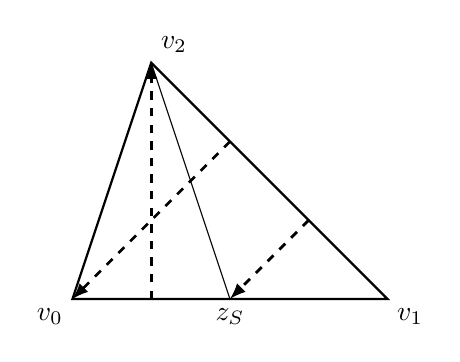
\begin{tikzpicture}
        % Coordinates of the triangle
        \coordinate (A) at (0,0); % Vertex A = v_0
        \coordinate (B) at (4,0); % Vertex B = v_1
        \coordinate (C) at (1,3); % Vertex C = v_2
        \coordinate (M) at ($(A)!0.5!(B)$); % Midpoint M of AB
        % Heights from each vertex
        \coordinate (H_A) at ($(C)!(A)!(B)$); % Height from A to BC
        \coordinate (H_B) at ($(C)!(B)!(A)$); % Height from B to AC
        \coordinate (H_C) at ($(A)!(C)!(B)$); % Height from C to AB
        \coordinate (H_M) at ($(B)!(M)!(C)$); % Height from M to BC
        % Drawing the triangle
        \draw[thick] (A) -- (B) -- (C) -- cycle;
        % Drawing the bisector from C to AB and the height vectors 
        %\draw[dashed] (C) -- (M);
        \draw[] (C) -- (M);
        \draw[dashed,->,line width=1.0pt,>=latex] (H_A) -- (A); % Height vector from A, original 
        \draw[dashed,->,line width=1.0pt,>=latex] (H_M) -- (M); % Height vector from A, original 
        \draw[dashed,->,line width=1.0pt,>=latex] (H_C) -- (C); % Height vector from C, unaffected
        % Marking the height points
        \node[above right] at (C) {$v_2$};  
        \node[below left] at (A) {$v_0$};
        \node[below right] at (B) {$v_1$};
        \node[below] at (M) {$z_S$};
    \end{tikzpicture}
    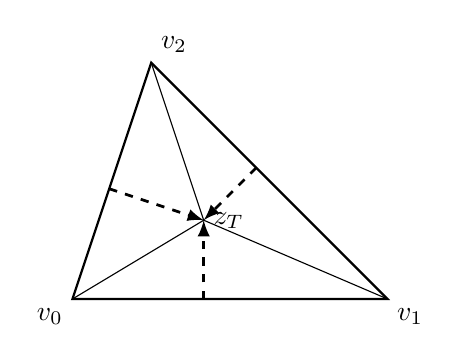
\begin{tikzpicture}

        % Coordinates of the triangle
        \coordinate (A) at (0,0); % Vertex A = v_0
        \coordinate (B) at (4,0); % Vertex B = v_1
        \coordinate (C) at (1,3); % Vertex C = v_2
        % Barycenter (centroid) of the triangle
        \coordinate (G) at (1.666666666,1); %($(A)!1/3!(B)!1/3!(C)$);
        % Drawing the triangle
        \draw[thick] (A) -- (B) -- (C) -- cycle;
        % Tripartitioning the triangle: draw lines from vertices to the barycenter
        \draw[] (A) -- (G);
        \draw[] (B) -- (G);
        \draw[] (C) -- (G);
        % Heights from the barycenter to the sides of the triangle
        \coordinate (H_GA) at ($(B)!(G)!(C)$); % Height from G to BC
        \coordinate (H_GB) at ($(A)!(G)!(C)$); % Height from G to AC
        \coordinate (H_GC) at ($(A)!(G)!(B)$); % Height from G to AB

        % Drawing the height vectors from the barycenter
        \draw[dashed,->,line width=1.0pt,>=latex] (H_GA) -- (G); % Height from G to BC
        \draw[dashed,->,line width=1.0pt,>=latex] (H_GB) -- (G); % Height from G to AC
        \draw[dashed,->,line width=1.0pt,>=latex] (H_GC) -- (G); % Height from G to AB

        % Marking the points
        \node[above right] at (C) {$v_2$};  
        \node[below left] at (A) {$v_0$};
        \node[below right] at (B) {$v_1$};
        \node[right] at (G) {$z_T$};
    \end{tikzpicture}
    \end{center}
    \caption{Illustration of Lemma~\ref{lemma:stardivision}. Left: 
	the triangle $T = [ v_0, v_1, v_2 ]$ is bisected at the edge $S = [ v_0, v_1 ]$, leading to two new triangles. 
	The height vector to $v_2$ in all three triangles remains the same. The height vector to $z_S$ in the new triangle $[z_S, v_1, v_2]$ is one half of the height vector to $v_0$ in the original triangle. 
	Right: 
	the triangle $T$ is trisected, leading to three new triangles. 
	The height vector to $z_T$ from the opposite edge in any triangle is one third of the original height vector of that edge.}
\end{figure}












We now provide the desired bi-Lipschitz transformation:
on the one hand, the nonlinear reflection across the interface between the selected simplex and the remainder of the local star,
and on the other hand, the bi-Lipschitz contraction from the local star onto the complement of the selected simplex. 
We give detailed estimates for the singular values of their Jacobians.

\begin{proposition}\label{proposition:starreflection}
    Let $\calT$ be a triangulation of an $n$-dimensional domain. 
    Let $S \in \calT$ be an inner simplex of dimension $k < n$,
    let $T \in \patch_{\calT}(S)$ be of dimension $n$,
    and let 
    \begin{align*}
        \Makoto := \overline{ \underlying{\patch_{\calT}(S)} \setminus T },
        \qquad 
        {\Gamma_1} := \Makoto \cap T,
        \qquad 
        {\Gamma_2} := \overline{ \partial T \setminus \partial \Makoto }.
    \end{align*}
    The following holds, where the constants on the right-hand sides are as stated in the proof. 
    \begin{enumerate}
    \item 
    There exists a bi-Lipschitz piecewise affine mapping
    \begin{align*}
        \Xi_{1} : T \rightarrow \Makoto
    \end{align*}
    which is the identity along ${\Gamma_1} = T \cap \Makoto$. 
    At any point, the singular values $\sigma_1 \geq \dots \geq \sigma_n$ of its Jacobian satisfy 
    \begin{gather*}
        \sigma_1 \leq \Cfive{n}{k}(\calT),
        \quad 
        \sigma_2,\dots,\sigma_n \leq \Cfiveprime{n}{k}(\calT),
        \quad 
        | \det\Jacobian\Xi_{1} |      \leq \Cdetfive{n}{k}(\calT),
        \\
        \sigma_n \leq \Csechs{n}{k}(\calT),
        \quad 
        \sigma_1^{-1},\dots,\sigma_{n-1}^{-1} \leq \Csechsprime{n}{k}(\calT),
        \quad 
        | \det\Jacobian\Xi_{1}^{-1} | \leq \Cdetsechs{n}{k}(\calT).
    \end{gather*}
%     and which satisfies the upper bounds 
%     \begin{gather*}
%         \matnorm{ \Jacobian\Xi_{1} }          \leq \Cfive{n}{k}(\calT),
%         \quad 
%         \matnorm{ \Jacobian\Xi_{1}^{-1} }     \leq \Csechs{n}{k}(\calT),
%         \\
%         | \det\Jacobian\Xi_{1} |      \leq \Cdetfive{n}{k}(\calT),
%         \quad 
%         | \det\Jacobian\Xi_{1}^{-1} | \leq \Cdetsechs{n}{k}(\calT).
%     \end{gather*}
    \item 
    There exists a bi-Lipschitz piecewise affine mapping
    \begin{align*}
        \Xi_{2} : \underlying{\patch_{\calT}(S)} \rightarrow \Makoto
    \end{align*}
    which is the identity along $\partial \Makoto \setminus \partial T$.
    At any point, the singular values $\sigma_1 \geq \dots \geq \sigma_n$ of its Jacobian satisfy 
    \begin{gather*}
        \sigma_1 \leq \Csieb{n}{k}(\calT),
        \quad 
        \sigma_2,\dots,\sigma_n \leq \Csiebprime{n}{k}(\calT),
        \quad 
        | \det\Jacobian\Xi_{2} |      \leq \Cdetsieb{n}{k}(\calT),
        \\
        \sigma_n \leq \Cacht{n}{k}(\calT),
        \quad 
        \sigma_1^{-1},\dots,\sigma_{n-1}^{-1} \leq \Cachtprime{n}{k}(\calT),
        \quad 
        | \det\Jacobian\Xi_{2}^{-1} | \leq \Cdetacht{n}{k}(\calT).
    \end{gather*}
%     and which satisfies the upper bounds 
%     \begin{gather*}
%         \matnorm{ \Jacobian\Xi_{2} }          \leq \Csieb{n}{k}(\calT),
%         \quad 
%         \matnorm{ \Jacobian\Xi_{2}^{-1} }     \leq \Cacht{n}{k}(\calT),
%         \\
%         | \det\Jacobian\Xi_{2} |      \leq \Cdetsieb{n}{k}(\calT),
%         \quad 
%         | \det\Jacobian\Xi_{2}^{-1} | \leq \Cdetacht{n}{k}(\calT).
%     \end{gather*}
    \end{enumerate}
\end{proposition}
\begin{proof}
    We derive the estimate in several steps. 
    In what follows, we use the notation $\hat z$ for the normalization of any vector $z \in \bbR^{n}$.
    \begin{itemize}
        \item 
        Without loss of generality, the barycenter $z_{S}$ of $S$ is the origin. 
        % Let $I := \Makoto \cap T$, which is the union of $k$ different faces of $T$, with $1 \leq k \leq n$.
        %We let ${\Gamma_2} \subseteq \partial T$ be the union of the remaining $n+1-k$ faces of $T$.
        %So ${\Gamma_2$} is within the boundary of the star $|\patch_{\calT}(S)|$ and is disjoint from $S$.
        We fix the subsimplex $S' \subseteq T$ that is complementary to $S$.
        Note that ${\Gamma_2}$ is the union of exactly those faces of $T$ that contain $S'$,
        whereas ${\Gamma_1} = \Makoto \cap T$ is the union of exactly those faces of $T$ that contain $S$. 
        
        
        \item 
        We let $z'_{S}$ be the midpoint of $S'$. 
        We apply barycentric refinement to the complementary simplex $S'$, which produces a new triangulation $\calS$. 
        Obviously, all $n$-simplices in $\calS$ contain $S$ and $z'_{S}$.
        
        We define another simplicial complex $\calS^c$ as follows:
        given any $n$-simplex $K \in \calS$, 
        we replace its vertex $z_{S}'$ by the new vertex $-z_{S}'$ at the opposite position,
        thus obtaining a new simplex $K'$. 
        Indeed, that $\calS^c$ is a simplicial complex follows easily from $\calS$ being a simplicial complex. 
        
        We let the simplicial complex $\calS'$ be the union of $\calS$ and $\calS^c$. 
        By construction, all its $n$-simplices contain $S$ as a subsimplex,
        % Indeed, $\calS'$ is indeed a triangulation since they are disjoint except for their proper subsimplices. 
        Moreover, $S$ is an inner subsimplex of that triangulation. 
        In particular, $\calS'$ is its own star around $S$.
        
        % TODO Check that $\calS'$ is a triangulation
        
        \item 
        As additional step, we introduce another simplicial complex $\calR'$ from $\calS'$ via barycentric subdivision of $S$.
        Then $\calR'$ is its own local star around the barycenter $z_S$.
        In particular, all $n$-simplices in $\calR'$ contain $z_{S}$. 
        The simplicial complex $\calR'$ also contains as subcomplexes the corresponding refinements of $\calS$ and $\calS^{c}$, 
        which we denote by $\calR$ and $\calR^{c}$, respectively.
        
        Lastly, we introduce one more simplicial complex $\calK$ obtained from $\patch_{\calT}(S)$ via barycentric refinement of $S$. 
        
        \item 
        We introduce a new mapping $\Theta : \underlying{\calR} \rightarrow \underlying{\calR^c}$ between the underlying sets as follows.
        Let $K \in \calR$ be an $n$-simplex and $K' \in \calR^{c}$ be constructed from $K$.
        We let $A_{K} : \Delta^{n} \rightarrow K$ and $A_{K'} : \Delta^{n} \rightarrow K'$
        be affine reference transformations
        that agree on the vertices common to $K$ and $K'$.
        Then the mapping 
        \begin{align*}
            \Theta_{|K} := A_{K'} \circ A_{K}^{-1}.
        \end{align*}
        % Notice that $A_{K'}$ and $A_{K}$ have the same singular values. Thus
        % \begin{align*}
        %     \matnorm{ \Jacobian \Theta_{|K}      } &\leq \| A_{K'} \| \cdot \| A_{K}^{-1} \| \leq \geometricshapemeasure(A_{K}),
        %     \\
        %     \matnorm{ \Jacobian \Theta_{|K}^{-1} } &\leq \| A_{K'}^{-1} \| \cdot \| A_{K} \| \leq \geometricshapemeasure(A_{K}).
        % \end{align*}
        preserves volumes:
        \begin{align*}
            |\det( \Jacobian      \Theta_{|K} )|
            = 
            |\det( \Jacobian^{-1} \Theta_{|K} )|
            =
            1
            .
        \end{align*}
        We want to characterize the singular values of this transform. 
        We $h_{z} \in \bbR^{n}$ be the height vector of $z_{S'}$ inside the simplex $K$.
        We can write
        \begin{align*}
            \Theta_{|K}(x) 
            = 
            x
            - 
            2 \frac{\langle \hat h_{z}, x \rangle}{\langle \hat h_{z}, \hat z_{S'} \rangle}
            \hat z_{S'}
            .
        \end{align*}
        Indeed, we check that the right-hand side equals $x$ whenever $x$ lies in the plane orthogonal to $h_{z}$,
        and that it equals $-z_{S'}$ when $x = z_{S'}$.
%         and when $x = z_{S'}$, then 
%         \begin{align*}
%             -z_{S'} 
%             =
%             z_{S'}
%             - 
%             2 \hat z_{S'} \frac{\langle \hat h_{z}, z_{S'} \rangle}{\langle \hat h_{z}, \hat z_{S'} \rangle}
%             .
%         \end{align*}
        If we orthogonally decompose $z_{S'} = h_{z} + b_{z}$ for some $b_{z} \in \bbR^{n}$, then 
        \begin{align*}
            \Theta_{|K}( h_{z} ) 
            &= 
            h_{z}
            - 
            2 \frac{\langle h_{z}, h_{z} \rangle}{\langle h_{z}, z_{S'} \rangle} z_{S'}
            = 
            h_{z}
            - 
            2 \frac{\langle h_{z}, z_{S'} \rangle}{\langle h_{z}, z_{S'} \rangle} z_{S'}
            %\\&
            = 
            h_{z}
            - 
            2 z_{S'}
            %\\&
            = 
            - h_{z}
            - 
            2 b_{z}
            .
        \end{align*}
        Evidently, the transformation $\Theta_{|K}$ equals the identity on the orthogonal complement of the span of $h_{z}$ and $b_{z}$. 
        Let $\beta$ be the angle between $z_{S'}$ and $h_{z}$. 
        Then $\vecnorm{ h_{z} } = \cos(\beta) \vecnorm{ z_{S'} }$ and $\vecnorm{ b_{z} } = \sin(\beta) \vecnorm{ z_{S'} }$. 
        We study the singular values of the matrix 
        \begin{align*}
            B 
            := 
            \begin{pmatrix}
            -1                 & 0
            \\ 
            -2 \vecnorm{ b_{z} }/\vecnorm{ h_{z} } & 1
            \end{pmatrix}
            =
            \begin{pmatrix}
            -1             & 0
            \\ 
            -2 \tan(\beta) & 1
            \end{pmatrix}
            .
        \end{align*}
        We compute the eigenvalues of the symmetric matrix $B^{\ast} B$. 
        Its square roots are the desired singular values of $B$:
        \begin{align}
            \sigma_{\max} = \sqrt{ 2\tan(\beta)^2 + 1 + 2 \tan(\beta) \sqrt{ \tan(\beta)^2 + 1 } } = \sqrt{ 1 + \tan^{2}(\beta) } + \tan(\beta) \label{math:theta_max}
            ,
            \\
            \sigma_{\min} = \sqrt{ 2\tan(\beta)^2 + 1 - 2 \tan(\beta) \sqrt{ \tan(\beta)^2 + 1 } } = \sqrt{ 1 + \tan^{2}(\beta) } - \tan(\beta) \label{math:theta_min}
            .
        \end{align}
        They are mutual reciprocals of each other and they monotonely increasing and decreasing, respectively, in $\tan(\beta)$.
        We conclude that these two are also the maximal and minimal singular values of $\Jacobian\Theta_{|K}$,
        whereas all its other singular values equal $1$. 
        
%         Let $\beta$ be the angle between $z_{S'}$ and $h_{z}$. 
        We develop explicit bounds for these singular values. 
        The definition of the tangent and the decomposition $z_{S'} = h_{z} + b_{z}$ 
        imply that $\tan(\beta) = \vecnorm{ b_{z} } / \vecnorm{ h_{z} }$.
        % Obviously, $\vecnorm{ b_{z} } \leq \vecnorm{ z_{S'} }$. 
        
        Recall that $K \in \calR$ is obtained from $T$ via barycentric subdivisions, first at $z_{S}$ and then at $z_{S'}$. 
        Let $F_{z} \subseteq K$ be the face opposite to the vertex $z_{S'}$,
        which must be contained in some face of $T$. 
        Since $S'$ has dimension $n-k-1$, the vector $(n-k) h_{z}$ is the height vector of that face of $T$. 
        Thus 
        \begin{align*}
            \frac{ \vecnorm{ b_{z} } }{ \vecnorm{ h_{z} } }
            = 
            \frac{ \vecnorm{ b_{z} } }{ (n-k)^{-1} \| (n-k) h_{z} \| }
            = 
            \frac{ \vecnorm{ z_{S'} } }{ (n-k)^{-1} \| (n-k) h_{z} \| }
            \leq 
            (n-k) \aspectratio(T)
%             = 
%             \frac{ \vecnorm{ b_{z} } \vol(F_{z}) }{ (n-k)^{-1} n \vol(T) }
%             \leq 
%             \frac{ n-k }{n!}
%             \cdot 
%             \frac{ \diam(T)^{n} }{ \vol(T) }
            .
        \end{align*}
        This establishes bounds on the singular values of the transformation. 
        We abbreviate 
        \begin{align}\label{math:upper_bound_for_theta}
            B_{T} 
            := 
%             \sqrt{ 1 + \tan^{2}(\beta) } - \tan(\beta) 
%             \geq 
            \sqrt{ 
                1 + (n-k)^{2} \aspectratio(T)^{2} % \frac{ \diam(T)^{2n} }{ n!^{2}\vol(T)^{2} } 
            } 
            + 
            (n-k) \aspectratio(T) % \frac{ \diam(T)^{n} }{ n! \vol(T) }            
            .
        \end{align}
        
        
        \item 
        We introduce another mapping $\Phi : \underlying{\calR'} \rightarrow \underlying{\calR^{c}}$ as follows. 
        Consider any $n$-simplex $K \in \calR$ and let $K^c \in \calR^{c}$ be its image under $\Theta$.
        We construct a bi-Lipschitz mapping 
        \begin{align*}
            \Phi_{K} : K \cup K^{c} \rightarrow K^{c}.
        \end{align*}
        The construction will be such that the union of $\Phi_{K}$ for all $n$-simplices $K \in \calR$
        will define the desired bi-Lipschitz mapping $\Phi : \underlying{\calR'} \rightarrow \underlying{\calR^{c}}$,
        which will be the identity along $\partial\underlying{\calR'} \setminus \partial\underlying{\calR}$.
        
        Once again, $h_{z}$ denotes the height of $z_{S'}$ within $K$.
        Here, we let $Q \subseteq K \cap K^{c}$ be the subsimplex 
        that is complementary to the line segment from the origin to $z_{S'}$ in $K$.
        Equivalently, $Q$ is complementary to the line segment from the origin to $-z_{S'}$ in $K^{c}$.
        From the very definition of simplices, we now conclude that any $x \in K \cup K^{c}$ 
        has a unique representation
        \begin{align*}
            x = \lambda z_{S} + \mu x^{Q}, \quad \lambda \in [-1,1], \quad \mu \in [0,1], \quad |\lambda| + \mu \leq 1, \quad x^{Q} \in Q,
        \end{align*}
        Since $\mu x^{Q}$ lies in the hyperplane spanned by the origin and $Q$, we have 
        \begin{align*}
            \lambda = \lambda(x) := \frac{\langle h_{z},x\rangle}{\langle h_{z},z_{S'}\rangle} 
            .
        \end{align*}
        Based on that observation, we define 
        \begin{align*}
            \Phi_{K}(x) 
            &
            := 
            \mu x^{Q} - \frac 1 2 \left( \lambda(x) - 1 \right) z_{S'}
            \\&
            = 
            x - \left( \frac 3 2 \lambda(x) - \frac 1 2 \right) z_{S'}
            = 
            x - \left( \frac 3 2 \frac{\langle h_{z},x\rangle}{\langle h_{z},z_{S'}\rangle} - \frac 1 2 \right) z_{S'}
            .
        \end{align*}
        We readily verify that this transformation is a bi-Lipschitz mapping from $K \cup K^{c}$ onto $K^{c}$
        that satisfies the desired mapping properties. 
        It remains to analyze its Jacobian to get explicit estimates. 
        
        We once more introduce an orthogonal decomposition $h_{z} + b_{z} = z_{S'}$ for some $b_{z} \in \bbR^{n}$.
        With that,
        \begin{align*}
            \Jacobian \Phi_{K}(x)
            &=
            \Id 
            - 
            \frac{3}{ 2 \langle h_{z},z_{S'}\rangle }  
            z_{S'} \otimes h_{z}^{t}
            \\
            &=
            \Id 
            - 
            \frac{3}{ 2 \langle h_{z},z_{S'}\rangle } 
            h_{z} \otimes h_{z}^{t}
            - 
            \frac{3}{ 2 \langle h_{z},z_{S'}\rangle } 
            b_{z} \otimes h_{z}^{t}
            \\
            &=
            \Id 
            - 
            \frac{3}{ 2 \langle h_{z}, h_{z}\rangle } 
            h_{z} \otimes h_{z}^{t}
            - 
            \frac{3}{ 2 \langle h_{z}, h_{z}\rangle } 
            b_{z} \otimes h_{z}^{t}
            \\
            &=
            \Id 
            - 
            \frac{3}{ 2 } 
            \hat h_{z} \otimes \hat h_{z}^{t}
            - 
            \frac{ 3 \vecnorm{ b_{z} } }{ 2 \vecnorm{ h_{z} } } 
            \hat b_{z} \otimes \hat h_{z}^{t}
            .
        \end{align*}
        The Jacobian acts as the identity over the span of $h_{z}$ and $z_{s'}$.
        We write $\beta$ for the angle between $h_{z}$ and $z_{S'}$.
        Hence $\tan(\beta) = \vecnorm{ b_{z} } / \vecnorm{ h_{z} }$. It remains to study the singular values of the matrix 
        \begin{align*}
            C 
            = 
            \begin{pmatrix}
                -\frac 1 2             & 0 
                \\
                -\frac 3 2 \tan(\beta) & 2 
            \end{pmatrix}
            = 
            \frac 1 2 
            \begin{pmatrix}
                -1 & 0 
                \\
                -3\tan(\beta) & 2 
            \end{pmatrix}
        \end{align*}
        By building the symmetric matrix $C^{t} C$ and computing its eigenvalues, we obtain 
        \begin{align*}
            \sigma_{\max} 
            = 
            \sqrt{ \frac{ \tan(\beta)^{2} + 5 }{8} + \frac 1 8 \sqrt{ \tan(\beta)^{4} + 10 \tan(\beta)^{2} + 9 } }
            =
            \frac 1 4 \sqrt{ 9 + \tan(\beta)^2 } + \frac 1 4 \sqrt{ 1 + \tan(\beta)^2 }
            ,
            \\
            \sigma_{\min} 
            = 
            \sqrt{ \frac{ \tan(\beta)^{2} + 5 }{8} - \frac 1 8 \sqrt{ \tan(\beta)^{4} + 10 \tan(\beta)^{2} + 9 } }
            =
            \frac 1 4 \sqrt{ 9 + \tan(\beta)^2 } - \frac 1 4 \sqrt{ 1 + \tan(\beta)^2 }
            .
        \end{align*}
        \begin{align*}
            \sigma_{\max} 
            = 
            \sqrt{ \frac{ 9\tan(\beta)^{2} + 5 }{8} + \frac 1 8 \sqrt{ 81\tan(\beta)^{4} + 90 \tan(\beta)^{2} + 9 } }
            %=
            %\frac 1 4 \sqrt{ 9 + 9\tan(\beta)^2 } + \frac 1 4 \sqrt{ 1 + 9\tan(\beta)^2 }
            =
            \frac 3 4 \sqrt{ 1 + \tan(\beta)^2 } + \frac 1 4 \sqrt{ 1 + 9\tan(\beta)^2 }
            ,
            \\
            \sigma_{\min} 
            = 
            \sqrt{ \frac{ 9\tan(\beta)^{2} + 5 }{8} - \frac 1 8 \sqrt{ 81\tan(\beta)^{4} + 90 \tan(\beta)^{2} + 9 } }
            =
            \frac 3 4 \sqrt{ 1 + \tan(\beta)^2 } - \frac 1 4 \sqrt{ 1 + 9\tan(\beta)^2 }
            .
        \end{align*}
        Notice that $\sigma_{\max} \sigma_{\min} = 1/2$. 
        These are monotonely increasing from $1$ and decreasing from $0.5$, respectively, in $\tan(\beta)$. 
        Hence, these are also the maximal and minimal eigenvalues of the Jacobian $\Jacobian \Phi_{K}$, the remaining eigenvalues being equal to $1$. Therefore,
        \begin{align*}
            \det \Jacobian\Phi = \frac 1 2.
        \end{align*}
        We now recall that the height of $h_{z}$ in $K \in \calR$ equals $(k+1)^{-1}$ multiplied with the height of some vertex of $S$ within $T$.
        Similar as above, we use the upper bound 
        \begin{align*}
            \tan(\beta) = \frac{\vecnorm{ b_{z} }}{\vecnorm{ h_{z} }} \leq (k+1) \aspectratio(T).
        \end{align*}
        We conclude that 
        \begin{gather}
            \matnorm{ \Jacobian\Phi_{K} } 
            \leq 
            \frac 3 4 \sqrt{ 1 + (k+1)^2 \aspectratio(T)^2 } + \frac 1 4 \sqrt{ 1 + 9(k+1)^2 \aspectratio(T)^2 }
            \leq 
            1 + \frac{3}{2} (k+1) \aspectratio(T) 
            \label{math:phi_max}
            ,
            \\
            \matnorm{ \Jacobian\Phi_{K}^{-1} } 
            \leq 
            \frac 3 2 \sqrt{ 1 + (k+1)^2 \aspectratio(T)^2 } + \frac 1 2 \sqrt{ 1 + 9(k+1)^2 \aspectratio(T)^2 }
            \leq 
            2 + 3 (k+1) \aspectratio(T) 
            \label{math:phi_min}
            .
        \end{gather}
        This finishes the discussion of the transformation $\Phi$.
        
        
        \item 
        We continue with an auxiliary result.
        Let $x, h_1, h_2 \in \bbR^{n}$ be non-zero. 
        Define 
        \begin{align*}
            F(x) 
            = 
            \frac{ \| h_2 \|^{2} }{ \langle h_2, x \rangle }
            \frac{ \langle h_1, x \rangle }{ \| h_1 \|^{2} }
            x
            .
        \end{align*}
        This is defined away from the hyperplane orthogonal to $h_2$.
        If $x \in \bbR^{n}$ with $\langle h_1, x \rangle = \| h_1 \|^{2}$, then $\langle F(x), h_2 \rangle = \| h_2 \|^{2}$.
        That shows that $F(x)$ is a radial mapping that maps each point on the hyperplane defined by the normal vector $h_1$
        onto the colinear point that lies on the hyperplane defined by the normal vector $h_2$. Indeed, 
        
        We identify the Lipschitz properties of this mapping by computing its Jacobian. 
        We write $\alpha_1, \alpha_2 \geq 0$ for the two angles between $h_1$ and $x$ and between $h_2$ and $x$, respectively. 
        In what follows, $y \in \bbR^{n}$.
        \begin{align*}
            \Jacobian F(x) \cdot y
            &=
            \frac{ \| h_2 \|^{2} }{ \langle h_2, x \rangle }
            \frac{ \langle h_1, y \rangle }{ \| h_1 \|^{2} }
            x
            - 
            \frac{ \langle h_2, h_2 \rangle \langle h_2, y \rangle }{ \langle h_2, x \rangle^{2} }
            \frac{ \langle x, h_1 \rangle }{ \langle h_1, h_1 \rangle }
            x 
            +
            \frac{ \langle h_2, h_2 \rangle }{ \langle h_2, x \rangle }
            \frac{ \langle x, h_1 \rangle }{ \langle h_1, h_1 \rangle }
            y 
            \\&=
            \frac{ \langle h_2, h_2 \rangle }{ \|h_2\| \|x\| \cos(\alpha_2) }
            \left( y - \frac{ \langle h_2, y \rangle }{ \langle h_2, x \rangle } x \right)
            \frac{ \langle x, h_1 \rangle }{ \langle h_1, h_1 \rangle }
            +
            \frac{ \| h_2 \|^{2} }{ \langle h_2, x \rangle }
            \frac{ \langle h_1, y \rangle }{ \| h_1 \|^{2} }
            x
            \\&=
            \frac{ \langle \hat h_2, h_2 \rangle }{ \cos(\alpha_2) }
            \left( y - \frac{ \langle \hat h_2, y \rangle }{ \langle \hat h_2, \hat x \rangle } \hat x \right)
            \frac{ \langle \hat x, \hat h_1 \rangle }{ \langle h_1, \hat h_1 \rangle }
            +
            \frac{ \| h_2 \| }{ \langle \hat h_2, \hat x \rangle }
            \frac{ \langle \hat h_1, y \rangle }{ \| h_1 \| }
            \hat x
            \\&=
            \frac{ \| h_2 \| }{ \cos(\alpha_2) }
            \left( y - \frac{ \langle \hat h_2, y \rangle }{ \cos(\alpha_2) } \hat x \right)
            \frac{ \cos(\alpha_1) }{ \| h_1 \| }
            +
            \frac{ \| h_2 \| }{ \cos(\alpha_2) }
            \frac{ \langle \hat h_1, y \rangle }{ \| h_1 \| }
            \hat x
            \\&=
            \frac{ \| h_2 \| }{ \| h_1 \| }
            \frac{ \cos(\alpha_1) }{ \cos(\alpha_2) }
            \left( 
                y 
                - 
                \frac{ \langle \hat h_2, y \rangle }{ \cos(\alpha_2) } \hat x 
                + 
                \frac{ \langle \hat h_1, y \rangle }{ \cos(\alpha_1) } \hat x 
            \right)
            .
        \end{align*}
        We define $a := \cos(\alpha_1)^{-1} \hat h_1 - \cos(\alpha_2)^{-1} \hat h_2$. 
        Notice that $a \perp \hat x$. The matrix $\Id + \hat x \otimes a^{t}$ is the identity over the orthogonal complement of the linear span of $a$ and $x$. Over that two-dimensional subspace, it can be represented by a triangular matrix.
        Similar as above, its largest and the smallest singular values $\sigma_{max} \geq 1 \geq \sigma_{\min}$ are
        %~\cite{blinn1996consider} 
        \begin{align*}
            \sigma_{\max} = \sqrt{ 1 + \frac{ \|a\|^{2} }{ 4 } } + \frac{ \|a\| }{2},
            \qquad 
            \sigma_{\min} = \sqrt{ 1 + \frac{ \|a\|^{2} }{ 4 } } - \frac{ \|a\| }{2}.     
        \end{align*}
        Notice that these are strictly monotonely increasing or decreasing, respectively, in $\|a\|$.
        We thus consider the upper bound 
        \begin{align*}
            \|a\| 
            \leq 
            2 \max_{1 \leq i \leq 2} 
            \left( 
                \frac{ \hat h_i }{ \langle \hat x, \hat h_i \rangle } 
            \right)
            .
        \end{align*}

        \item 
        We now describe the construction of a bi-Lipschitz mapping 
        \begin{align*}
            \Psi : \underlying{\calR'} \rightarrow \underlying{\calK}.
        \end{align*}
        Recall that $\calR'$ and $\calK$ are their own respective stars around the origin,
        so they must contain an open ball around the origin. 
        % TODO \mwl{Here we need to show that it is indeed a ball. It must be a domain triangulation.}
        Let ${G} \in \calR'$ be an $n$-dimensional simplex and let $x \in {G}$ be non-zero. There exists a simplex $K \in \calK$ that intersects the ray $\bbR_0^+ \cdot x$. We let $h_{{G}}$ and $h_{K}$ be the normals of the origin within ${G}$ and $K$, respectively. They define respective hyperplanes $H_{G}$ and $H_{K}$,
        and we write $F_{G} = G \cap H_{G}$ and $F_{K} = K \cap H_{K}$ for the corresponding faces. 
        We notice that $x$ has a sharp angle to both $h_{{G}}$ and $h_{K}$,
        that is, the scalar product of $x$ with either height vector is positive. 
        We define 
        \begin{align*}
            \Psi(x) 
            = 
            \frac{ \| h_K \|^{2} }{ \langle h_K, x \rangle }
            \frac{ \langle h_{{G}}, x \rangle }{ \| h_{{G}} \|^{2} }
            x
            .
        \end{align*}
        One easily verifies that this defines a continuous mapping $\Psi$. 
        By the same line of thought, we see that it is invertible with inverse satisfying 
        \begin{align*}
            \Psi^{-1}(z) 
            = 
            \frac{ \| h_{{G}} \|^{2} }{ \langle h_{{G}}, z \rangle }
            \frac{ \langle h_K, z \rangle }{ \| h_K \|^{2} }
            z,
            \qquad 
            z = \Psi(x)
            .
        \end{align*}
        We let $\alpha_K$ and $\alpha_{{G}}$ be the angles of $x$ with the vectors $h_{{G}}$ and $h_{K}$, respectively,
        and let 
        \begin{align*}
            a := \cos(\alpha_{{G}})^{-1} \hat h_{{G}} - \cos(\alpha_K)^{-1} \hat h_K
            .
        \end{align*}
        The preceding auxiliary results now contribute all information on the singular values of these Jacobians:
        \begin{gather*}
            \matnorm{ \Jacobian\Psi(x) }
            = 
            \frac{ \| h_K \| }{ \| h_{{G}} \| }
            \frac{ \cos(\alpha_{{G}}) }{ \cos(\alpha_K) }
            \left( 
                \sqrt{ 1 + \frac{ \|a\|^{2} }{ 4 } } + \frac{ \|a\| }{2}
            \right)
            \\
            \matnorm{ \Jacobian\Psi(z)^{-1} }
            = 
            \frac{ \| h_{{G}} \| }{ \| h_K \| }
            \frac{ \cos(\alpha_K) }{ \cos(\alpha_{{G}}) }
            \left( 
                \sqrt{ 1 + \frac{ \|a\|^{2} }{ 4 } } - \frac{ \|a\| }{2}
            \right)^{-1},
            \\
            \det\Jacobian\Psi(x)
            =
            \left( 
            \frac{ \| h_K \| }{ \| h_{{G}} \| }
            \frac{ \cos(\alpha_{{G}}) }{ \cos(\alpha_K) }
            \right)^{n},
            \qquad
            \det\Jacobian\Psi^{-1}(x)
            =
            \left( 
            \frac{ \| h_{{G}} \| }{ \| h_{K} \| }
            \frac{ \cos(\alpha_{K}) }{ \cos(\alpha_{{G}}) }
            \right)^{n}
        \end{gather*}
        We let $x_{G} \in F_{G}$ and $x_{K} \in F_{K}$ be the intersection points of the ray $\bbR \cdot x$ with the respective faces.
        By the definition of the cosine, 
        \begin{align*}
            \frac{ \| h_K \| }{ \| h_{{G}} \| }
            \frac{ \cos(\alpha_{{G}}) }{ \cos(\alpha_K) }
            = 
            \frac{ \| x_K \| }{ \| x_{{G}} \| }
            \leq 
            \frac{ \| x_K \| }{ \| h_{{G}} \| }
            \leq 
            \frac{ \diam(K) }{ \| h_{{G}} \| }
            ,
            \qquad 
            \frac{ \| h_{{G}} \| }{ \| h_K \| }
            \frac{ \cos(\alpha_K) }{ \cos(\alpha_{{G}}) }
            = 
            \frac{ \| x_{G} \| }{ \| x_{K} \| }
            \leq 
            \frac{ \| x_{G} \| }{ \| h_{K} \| }
            \leq 
            \frac{ \diam(G) }{ \| h_{K} \| }
            .
        \end{align*}
%         \begin{align*}
%             \frac{ \| h_K \| }{ \| h_{{G}} \| }
%             \frac{ \cos(\alpha_{{G}}) }{ \cos(\alpha_K) }
%             \leq 
%             \frac{ \| x_K \| }{ \| x_{{G}} \| }
%             .
%         \end{align*}
        We need further details to complete our estimates. 
        We know that $\| x_K \| \leq \diam(K)$ and that the diameters of the simplices in $\calK$ are already bounded by the maximum diameter in $\patch_{\calT}(S)$. The height $h_{K}$ is obtained from a height vector of a vertex in $\patch_{\calT}(S)$ by scaling with the factor $(k+1)^{-1}$.
        That estimates the quotient $\| x_K \| / \| h_K \|$. 
        % 
        In oder to estimate $\|x_{G}\|$, we first notice the case $G \in \calR$ implies $\|x_{G}\| \leq \diam(G) \leq \diam(T)$. 
        In the case $G \in \calR^{c}$, we recall that $x = \lambda (-z_{S'}) + (1-\lambda) z_{x}$ for some $\lambda \in [0,1]$ and $z_{x} \in G$
        that must lie in the face of $G$ that is opposite to $-z_{S'}$. 
        The preimage of $x$ under $\Theta_{{G}}$ is $\lambda z_{S'} + (1-\lambda) z_{x}$. 
        It follows again that $\|x_{G}\| \leq \diam(T)$. 
        % 
        It remains to find a lower bound for $\| h_{G} \|$.
        Every height of the origin in some simplex of $\calR'$ is obtained from a height vector of some vertex in $S$ in some simplex in $\calS'$
        by scaling with $(k+1)^{-1}$. If $G \in \calR$, then that original height was already a height of a vertex of $S$ in $T$. 
        If instead $G \notin \calR$, then each of the latter height vectors has length bounded from below by the height of some vertex in $S$ within a simplex of $\calS$, multiplied by $B_{T}$. The height of any vertex of $S$ in some simplex of $\calS$ is the same as the height $h_T$ of that vertex in the original simplex $T$. 
        %         In oder to estimate $\|x_{G}\|$, recall that $x = \lambda (-z_{S'}) + (1-\lambda) z_{x}$ for some $\lambda \in [0,1]$ and $z_{x} \in G$
        %         being in the face of $G$ that is opposite to $z_{x}$. The preimage of $x$ under $\Theta_{{G}}$ is $\lambda z_{S'} + (1-\lambda) z_{x}$. 
        %         It follows that $\|x_{G}\| \leq \diam(T)$. 
        %         
%         We know that whenever $T$ is a simplex with some face $F$ and $h_F$ is corresponding height vector, then 
%         \begin{align*}
%             \frac{\diam(T)}{ \|h_{F}\|}
%             \leq  
%             \aspectratio(T)
%             % \frac{ \vol(F) \diam(T) }{ n \vol(T) } \leq \frac{ \diam(T)^{n} }{ n! \vol(T) }
%             .
%         \end{align*}
        Putting all these technical observations together, we estimate 
        \begin{align*}
            \frac{ \| x_{K} \| }{ \| h_{{G}} \| }
            &\leq 
            (k+1)B_{T}
            \frac{ \diam(K) }{ \| h_{T} \| }
            \leq 
            (k+1)B_{T}
            \diameterratio(\calT)
            \frac{ \diam(T) }{ \| h_{T} \| }
            \leq 
            (k+1)B_{T}
            \diameterratio(\calT)
            \aspectratio(T) % \frac{ \diam(T)^{n} }{ n! \vol(T) }
            ,
            \\
            \frac{ \| x_{G} \| }{ \| h_{K} \| }
            &\leq 
            (k+1)
            \sup_{ K \in \patch_{\calT}(S) }
            \frac{ \diam(T) }{ \| h_{K} \| }
            \leq 
            (k+1)
            \diameterratio(\calT)
            \sup_{ K \in \patch_{\calT}(S) }
            \frac{ \diam(K) }{ \| h_{K} \| }
            \leq 
            (k+1)
            \diameterratio(\calT)
            \sup_{ K \in \patch_{\calT}(S) }
            \aspectratio(K) % \frac{ \diam(K)^{n} }{ n! \vol(K) }
            .
        \end{align*}
        \begin{gather*}
            \frac{ \| x_{K} \| }{ \| h_{{K}} \| }
            \leq 
            (k+1)
            \sup_{ K \in \patch_{\calT}(S) }
            \aspectratio(K) % \frac{ \diam(K)^{n} }{ n! \vol(K) }
            ,
            \qquad 
            \frac{ \| x_{G} \| }{ \| h_{G} \| }
            \leq 
            (k+1)B_{T}
            \aspectratio({G}) % \frac{ \diam(T)^{n} }{ n! \vol(T) }
            .
        \end{gather*}

        
        %         To simplify that expression, we make another observation regarding the height vectors. 
        %         when $T$ is an $n$-dimensional simplex with a $k$-dimensional subsimplex $S \subseteq T$,
        %         and $h > 0$ is the height of some vertex $v \in S$ opposite to a face $F$,
        %         then the barycenter $z_S$ of $S$ has distance $h/(k+1)$ from the face $F$. 
        %         From this observation we infer that the height vectors at the origin of the simplices in $\calR'$ and $\calK$
        %         are obtained by rescaling the height vectors in $\calS'$ and $\patch_{\calT}(S)$
        %         with the factor $(k+1)^{-1}$.
        
        The vector $a$ is the difference between $\hat h_{G}$ and $\hat h_{K}$ after both are rescaled such that they lie on the affine hyperplane with normal vector $\hat x$. That difference has length at most $\tan(\alpha_{G}) + \tan(\alpha_{K})$.
        We calculate 
        \begin{align*}
            \|a\|
            = 
            \left\|
            \frac{\|x_{G}\|}{\|h_{G}\|} \hat h_{{G}} 
            - 
            \frac{\|x_{K}\|}{\|h_{K}\|} \hat h_K
            \right\|
            &
            \leq 
            \frac{\|x_{G}\|}{\|h_{G}\|} 
            + 
            \frac{\|x_{K}\|}{\|h_{K}\|} 
            % \\&
            \leq 
            (k+1) 
            \left( 1 + B_{T} \right)
            \sup_{ K \in \patch_{\calT}(S) }
            \aspectratio(K) % \frac{ \diam(K)^{n} }{ n! \vol(K) }
            .
        \end{align*}
        In summary, using that $\sqrt{s^2+t^2} \leq s + t$ for any $s,t \geq 0$, we find the upper bounds 
        \begin{align*}
            \matnorm{ \Jacobian\Psi(x) }
            &\leq  
            (k+1)B_{T}
            \diameterratio(\calT)
            \aspectratio(T) % \frac{ \diam(T)^{n} }{ n! \vol(T) }
            \cdot 
            \left( 
                1 
                + 
                (k+1) 
                \left( 1 + B_{T} \right)
                \aspectratio(\calT) 
            \right)
            ,
            \\
            \matnorm{ \Jacobian\Psi(z)^{-1} }
            &\leq  
            (k+1)
            \diameterratio(\calT)
            \aspectratio(\calT) 
            \cdot 
            \left( 
                1 
                + 
                (k+1) 
                \left( 1 + B_{T} \right)
                \aspectratio(\calT) 
            \right)
            ,
            \\
            \det\Jacobian\Psi(x)
            &\leq 
            \left( 
            (k+1)B_{T}
            \diameterratio(\calT)
            \aspectratio(T) % \frac{ \diam(T)^{n} }{ n! \vol(T) }
            \right)^{n},
            \\
            \det\Jacobian\Psi^{-1}(x)
            &\leq 
            \left( 
            (k+1)
            \diameterratio(\calT)
            \aspectratio(\calT) 
            \right)^{n}
        \end{align*}
        We have shown that $\Psi$ and $\Psi^{-1}$ are piecewise Lipschitz with respect to some essentially disjoint closed partitions over their respective domains.
        % It remains to show both are Lipschitz, which we illustrate for $\Psi$, the argument for $\Psi^{-1}$ being analogous. 
        % Rademacher's theorem then shows that both have essentially bounded weak Jacobians. 
        Every function that is piecewise Lipschitz with respect to the triangulation $\calK$ must be Lipschitz over all of $\underlying{\calK}$, since there exists a bi-Lipschitz transformation from $\underlying{\calK}$ onto the unit ball.
        % We use a technique similar to Lemma~\ref{lemma:stars_are_shellable}. 
        % After application of a piecewise linear Lipschitz mapping, 
        % we can assume that $\underlying{\calK}$ is convex without loss of generality. 
        % Any function piecewise Lipschitz with respect to $\calK$ must be Lipschitz over $\underlying{\calK}$. 
        % \mwl{TODO: not enough. Instead, use the homeomorphism onto a ball and estimate its Lipschitz constant.}
        
        
        \item 
        We define a mapping $ \Xi_{1} : T \rightarrow \Makoto = \overline{ \underlying{ \patch_{\calT}(S) } \setminus T}$ by setting 
        \begin{align*}
            \Xi_{1} := \Psi \circ \Theta.
        \end{align*}
        It preserves the interface from $T$ onto $\Makoto$. 
        Let $\sigma_1(x) \geq \dots \geq \sigma_n(x)$ be the singular values of its Jacobian at $x \in T$. 
        Combining the previous estimates for $\Psi$ and $\Theta$ with interlacing inequalities for the singular values of product matrices provides 
        \begin{align*}
            \sigma_1(x) = \matnorm{ \Jacobian \Xi_{1} }
            &\leq 
            \Cfive{n}{k}(\calT)
            :=
            (k+1) 
            \diameterratio(\calT)
            \aspectratio(\calT)
            B_{T}^{2}
            \Big( 
                1 
                + 
                (k+1) 
                \left( 1 + B_{T} \right)
                \aspectratio(\calT)
            \Big)            
            ,
            \\
            \sigma_2(x), \dots, \sigma_n(x) 
            &\leq 
            \Cfiveprime{n}{k}(\calT)
            :=
            (k+1)B_{T}
            \diameterratio(\calT)
            \aspectratio(T) 
            \cdot 
            B_T
            \\
            \sigma_n(x)^{-1} = \matnorm{ \Jacobian \Xi_{1}^{-1} }
            &\leq
            \Csechs{n}{k}(\calT)
            :=
            (k+1) 
            \diameterratio(\calT)
            \aspectratio(\calT)
            B_{T}
            \Big( 
                1 
                + 
                (k+1) 
                \left( 1 + B_{T} \right)
                \aspectratio(\calT)
            \Big)
            \\
            \sigma_1(x)^{-1}, \dots, \sigma_{n-1}(x)^{-1}
            &\leq 
            \Csechsprime{n}{k}(\calT)
            :=
            (k+1)
            \diameterratio(\calT)
            \aspectratio(\calT) 
            \cdot 
            B_T
            .
        \end{align*}
        We get the determinant estimates
        \begin{align*}
            |\det(\Xi_{1})|
            &\leq 
            \Cdetfive{n}{k}(\calT)
            :=
            (k+1)^{n}
            \diameterratio(\calT)^{n}
            B_{T}^{n}
            \aspectratio(\calT)^{n}
            ,
            \\
            |\det(\Xi_{1}^{-1})|
            &\leq 
            \Cdetsechs{n}{k}(\calT)
            :=
            (k+1)^{n}
            \diameterratio(\calT)^{n}
            \aspectratio(\calT)^{n}
            .
        \end{align*}
        This completes the desired estimates for $\Xi_{1}$. 
        
        
        \item 
        We define another mapping $ \Xi_{2} : \underlying{\patch_{\calT}(S)} \rightarrow \Makoto $ by setting 
        \begin{align*}
            \Xi_{2} := \Psi \circ \Phi.
        \end{align*}
        It is bi-Lipschitz and preserves $\partial\underlying{\patch_{\calT}(S)} \setminus \partial T$. 
        Let $\sigma_1(x) \geq \dots \geq \sigma_n(x)$ be the singular values of its Jacobian at $x \in \underlying{\patch_{\calT}(S)}$. 
        The combination of the previous estimates for $\Psi$ and $\Phi$ with standard interlacing inequalities now lead to 
        \begin{align*}
            \sigma_1(x)
            = 
            \matnorm{ \Jacobian \Xi_{2} }
            &\leq 
            \Csieb{n}{k}(\calT)
            :=
            \left( 1 + \frac{3}{2} (k+1) \aspectratio(T) \right)
            \cdot 
            (k+1) 
            \aspectratio(\calT)
            B_{T}
            \Big( 
                1 
                + 
                (k+1) 
                \left( 1 + B_{T} \right)
                \aspectratio(\calT)
            \Big)            
            \\
            \sigma_2(x), \dots, \sigma_n(x) 
            &\leq 
            \Csiebprime{n}{k}(\calT)
            :=
            (k+1)B_{T}
            \diameterratio(\calT)
            \aspectratio(T) 
            \cdot 
            \left( 1 + \frac{3}{2} (k+1) \aspectratio(T) \right)
            \\
            \sigma_n(x)^{-1}
            = 
            \matnorm{ \Jacobian \Xi_{2}^{-1} }
            &\leq  
            \Cacht{n}{k}(\calT)
            :=
            \left( 2 + 3 (k+1) \aspectratio(T) \right)
            \cdot 
            (k+1) 
            \aspectratio(\calT)
            \Big( 
                1 
                + 
                (k+1) 
                \left( 1 + B_{T} \right)
                \aspectratio(\calT)
            \Big)            
            \\
            \sigma_1(x)^{-1}, \dots, \sigma_{n-1}(x)^{-1}
            &\leq 
            \Cachtprime{n}{k}(\calT)
            :=
            (k+1)
            \diameterratio(\calT)
            \aspectratio(\calT) 
            \cdot 
            \left( 2 + 3 (k+1) \aspectratio(T) \right)
            .
        \end{align*}
        We get the determinant estimates 
        \begin{align*}
            |\det(\Xi_{2})|
            &\leq 
            \Cdetsieb{n}{k}(\calT)
            :=
            \frac 1 2 
            (k+1)^{n}
            \diameterratio(\calT)^{n}
            B_{T}^{n}
            \aspectratio(\calT)^{n}
            ,
            \\
            |\det(\Xi_{2}^{-1})|
            &\leq 
            \Cdetacht{n}{k}(\calT)
            :=
            2
            (k+1)^{n}
            \diameterratio(\calT)^{n}
            \aspectratio(\calT)^{n}
            .
        \end{align*}
        This completes the desired estimates for $\Xi_{2}$. 
    \end{itemize}
    The proof is complete. 
\end{proof}
        

\begin{remark}
    We notice that the mappings $\Xi_{1}$ and $\Xi_{2}$ above are not only bi-Lipschitz, but in fact also piecewise affine, 
    where piecewise refers to an essentially non-overlapping decomposition of their respective domains into convex polytopes.
    While the reflection and deformation mappings in Proposition~\ref{proposition:starreflection} serve our purpose,
    it might be possible to improve the analysis or construction and lower the Jacobian estimates. 
\end{remark}



        
        
        
        





        
        
        
        








































\section{Constructive estimates of Poincar\'e--Friedrichs constants}\label{section:poincarefriedrichs}

We are now in the position to develop Poincar\'e--Friedrichs constants for the exterior derivative over domains with shellable triangulations; this includes the curl and divergence operators in three dimensions. 
These results use local Poincar\'e--Friedrichs constants over simplices, 
with or without boundary conditions, as subcomponents. 

The analysis of the Poincar\'e potential operators in Section~\ref{section:potentialoperator}
implies the following estimate for Poincar\'e--Friedrichs constants over convex domains. 

\begin{lemma}\label{lemma:PFexteriorsimplex}
    Let $\Omega \subseteq \bbR^{n}$ be a convex bounded open set. 
    Let $0 \leq k < n$. 
    Then for each $u \in W^{p}\Lambda^{k}(\Omega)$ 
    there exists $w \in W^{p}\Lambda^{k}(\Omega)$ 
    with $\cartan u = \cartan w$ and 
    \begin{align*}
        \| w \|_{L^{p}(\Omega)}
        &
        \leq 
        C_{{\PF},k,\Omega,p}
        \| \cartan u \|_{L^{p}(\Omega)}
        .
    \end{align*}
    where 
    \begin{align*}
        C_{{\PF},k,\Omega,p} 
        = 
        n C_{\Poinc}(n,k+1) 
        \vol_{}(B_1(0)) 
        \frac{ \diam(\Omega)^{n} }{ \vol(\Omega) } 
        \diam(\Omega)
        .
    \end{align*}
\end{lemma}
\begin{proof}
    This follows from Theorem~\ref{theorem:bogovpoinc} using $\vol(B_{\diam(\Omega)}(0)) = \vol_{}(B_1(0)) \diam(\Omega)^{n}$.
\end{proof}

We also need a Poincar\'e--Friedrichs inequality for differential forms over a simplex but subject to homogeneous boundary conditions along a collection of faces. 

\begin{lemma}\label{lemma:mixedbconsimplex:exteriorderivative}
    Let $T$ be an $n$-simplex 
    and let $\Gamma = F_{0} \cup \dots \cup F_{\ell}$ be the union of $\ell+1$ different faces of $T$. 
    Suppose that $u \in W^{p}\Lambda^{k}(T)$ such that 
    $\trace_{T,\Gamma} u = 0$.
    Then there exists $w \in W^{p}\Lambda^{k}(T)$ such that 
    $\trace_{T,\Gamma} w = 0$
    and  
    \begin{align*}
        \cartan w = \cartan u,
        \quad 
        \| w \|_{L^{p}(\Omega)} 
        \leq 
        C_{\PF,\Gamma,\ell,k,p}(T)
        \| \cartan u \|_{L^{p}(\Omega)}
        .
    \end{align*}
    Here, $C_{\PF,\Gamma,\ell,k,p}(T) > 0$ is a constant such that 
    \begin{align*}
        C_{\PF,\Gamma,\ell,k,p}(T)
        \leq 
        2^{\frac{n-\ell}{p}}
        2^{n+1} n C_{\Bogov}(n,k+1) \frac{ \vol_{}(B_1(0)) }{ (\ell+1)/n! } 
        \algebraicshapemeasure(T)^{k-1}
        \Ceins{n}(T) 
        \diam(T)
        .
    \end{align*}
\end{lemma}
\begin{proof}
    There exists an affine bijection $\varphi : \Delta^n \rightarrow T$ 
    that maps the convex closure of the $n$ unit vectors onto the face $F_0$.
    We can also assume that the face of $\Delta^n$
    orthogonal to the $i$-th coordinate axis is mapped 
    onto the face $F_i$. 
    In what follows, we let $\widetilde \Makoto$ be the convex set obtained from reflecting $\Delta^n$ along the coordinate axes $l+1$ through $n$. 
    We see that $\vol(\widetilde \Makoto) = (l+1)/n!$
    
    We let $\hat u := \varphi^{\ast} u$ and define $\hat g \in L^{p}(\Delta^n)$ via $\hat g := \cartan \varphi^{\ast} u$. 
    Then $\cartan \hat u = \hat g$. 
    We let $\tilde u$ be the extension of $\hat u$ onto $\widetilde \Makoto$ by reflection across the coordinate axes,
    and let $\tilde g$ is the extension of $\hat g$ onto $\widetilde \Makoto$ by reflection across the coordinate axes. 
    We observe $\tilde g = \cartan \tilde u$. 
    By construction, $\tilde u \in W^{p}_{0}\Lambda^{k}(\widetilde \Makoto)$.
    
    The bounds for the Bogovski\u{i} potential operators, Theorem~\ref{theorem:bogovpoinc} imply 
    the existence of $\tilde w \in W^{p}_{0}\Lambda^{k}(\widetilde \Makoto)$
    with $\cartan \tilde w = \cartan \tilde u$ and 
    \begin{align*}
        \| \tilde w \|_{L^{p}(\widetilde \Makoto)}
        &\leq 
        n C_{\Bogov}(n,k+1) \frac{ \vol_{}(B_2(0)) }{ \vol(\widetilde \Makoto) } 
        2
        \| \tilde g \|_{L^{p}(\widetilde \Makoto)}
        \\&\leq 
        2^{n+1} n C_{\Bogov}(n,k+1) \frac{ \vol_{}(B_1(0)) }{ (l+1)/n! } 
        \| \tilde g \|_{L^{p}(\widetilde \Makoto)}
        .
    \end{align*}
    We let $w \in W^{p}\Lambda^{k}(T)$ be defined by $w := \varphi^{-\ast} ( \tilde w_{|\Delta^n} )$.
    By construction, $\cartan w = \cartan u$,
    and $w$ has vanishing trace along $F_{0} \cup \dots \cup F_{l}$.
    
    In addition to that, by Proposition~\ref{proposition:pullbackestimate}:
    \begin{align*}
        \| w \|_{L^{p}(T)}
        &\leq 
        |\det(\Jacobian \varphi)|^{\frac 1 p} 
        \matnorm{ \Jacobian \varphi^{-1} }^{k-1}
        \| \tilde w \|_{L^{p}(\Delta^n)}
        ,
        \\
        \| \tilde g \|_{L^{p}(\widetilde \Makoto)}
        \leq 
        2^{\frac {n-\ell} p}
        \| \hat g \|_{L^{p}(\Delta^n)}
        &\leq 
        2^{\frac {n-\ell} p}
        |\det( \Jacobian \varphi^{-1} )|^{\frac 1 p} 
        \matnorm{\Jacobian \varphi}^{k}
        \cdot 
        \| \cartan u \|_{L^{p}(T)}
        .
    \end{align*}
    It remains to use Lemma~\ref{lemma:measurerelationships}, and the desired inequality is shown. 
\end{proof}


We prepare some further notation for our two main results. 
Whenever $\calT$ is an $n$-dimensional triangulation, we use the abbreviation
\begin{align*}
    C_{\PF,\Gamma,k,p}(\calT) 
    :=
    \max\limits_{ \substack{ T \in \calT \\ \dim(T)=n \\ 0 \leq l \leq n } }
    C_{\PF,\Gamma,l,k,p}(T)
    .
\end{align*}
Suppose that $\calT$ is an $n$-dimensional triangulation and has a shelling $T_{0}, T_{1}, \dots, T_{M}$. 
For each $0 \leq m \leq M$, we write 
\begin{align*}
    X_{m} := T_0 \cup T_1 \cup \dots \cup T_{m},
\end{align*}
which is by Lemma~\ref{lemma:shell_triang_man} a triangulated $n$-dimensional submanifold with boundary. 
For each $1 \leq m \leq M$, the interface of the new simplex to the previous intermediate triangulation is 
\begin{align*}
    \Gamma_{m} := T_{m} \cap X_{m-1} %\left( T_{0} \cup \dots \cup T_{m-1} \right)
    .
\end{align*}
According to Lemma~\ref{lemma:existenceofstar}, 
there exists an interior simplex $S_{m} \in \calT$ 
such that $T_{m}$ is the last $n$-simplex in the shelling that belongs to $T_{m} \in \patch_{\calT}(S_{m})$.
In particular, already $\patch_{\calT}(S_{m}) \subseteq X_{m}$. % is already included in the union of the simplices up to $T_m$. 

In addition to that, we introduce 
\begin{align*}
    \Makoto_{m-1} := \patch_{\calT}(S_{m}) \setminus T_{m}.
\end{align*}
for the complement $\Makoto_{m-1} \subseteq X_{m-1}$ of the simplex $T_{m}$ in the star $\patch_{\calT}(S_{m})$. 

The two main results of this manuscript for shellable triangulations of domains, not necessarily convex or even star-shaped, is the following theorems. 
The first one is inspired by the recursive construction of gradient potentials in Theorem~\ref{theorem:poincarefriedrichsestimate:grad}.
The second one is specific to the fact that shellable triangulations are contractible.




\begin{theorem}\label{theorem:poincarefriedrichsestimate:exterior}
    % Let $\Omega \subseteq \bbR^{n}$ be a domain with a shellable $n$-dimensional triangulation $\calT$.
	Let $\calT$ be a shellable $n$-dimensional triangulation, and let the domain $\Omega \subseteq \bbR^{n}$ be the interior of the underlying set of $\calT$.
    Let $T_0, T_1, \dots, T_M$ be a shelling.
    Then for any $u \in W^{p}\Alt^{k}(\Omega)$ 
    there exists $w \in W^{p}\Alt^{k}(\Omega)$ with $\cartan w = \cartan u$
	and such that the following estimates hold:
	\begin{gather*}
        \| w_0 \|_{L^{p}(T_{0})} \leq C_{{\PF},k,T_{0},p} \| \cartan u \|_{L^{p}(T_{0})}.
    \end{gather*}
    and for each $T_{m} \in \calT$, $1 \leq m \leq M$ we have the recursive estimate 
    \begin{align*}
        \| w \|_{L^{p}(T_{m})}
        &
        \leq  
        C_{\PF,T_{m},\Gamma_{m},k,p}(\calT) 
        \left( 
            \| \cartan u      \|_{L^{p}(T_{m})} 
            +
            \Cfive{n}{k}(\calT)
            \Cfiveprime{n}{k}(\calT)^{k} 
            \Cdetsechs{n}{k}(\calT)^{\frac 1 p} 
            \| \cartan u \|_{L^{p}(\Makoto_{m-1})}
        \right)
        \\&\qquad
        + 
        \Cfive{n}{k}(\calT) 
        \Cfiveprime{n}{k}(\calT)^{k-1} 
        \Cdetsechs{n}{k}(\calT)^{\frac 1 p} 
        \| w \|_{L^{p}(\Makoto_{m-1})}
        .
    \end{align*}
\end{theorem}
\begin{proof}
    Let $u \in W^{p}\Alt^{k}(\Omega)$. 
    First, there exists $w_0 \in W^{p}\Alt^{k}(T_{0})$ satisfying $\cartan w_0 = \cartan u$ over $T_{0}$ together with 
    \begin{gather*}
        \| w_0 \|_{L^{p}(T_{0})} \leq C_{{\PF},k,T_{0},p} \| \cartan u \|_{L^{p}(T_{0})}.
    \end{gather*}
    Suppose that $0 < m \leq M$ such that there exists $w_{m-1} \in W^{p}\Alt^{k}(X_{m-1})$ 
    with $\cartan w_{m-1} = \cartan u$ over $X_{m-1}$. 
    By assumption, $T_{m}$ and $X_{m-1}$ share the interface $\Gamma_{m}$, which is a collection of faces of $T_{m}$. 
    In accordance to Lemma~\ref{lemma:existenceofstar}, adding $T_{m}$ completes a star in $\calT$ around some simplex $S_{m}$, 
	and we let $\Makoto_{m-1} \subseteq X_{m-1}$ be the complement of $T_{m}$ in that newly completed star. 
    
    We introduce the reflection mapping $\Xi_{1} : T_{m} \rightarrow \Makoto_{m-1}$ of Proposition~\ref{proposition:starreflection}. 
    We define $w'_{m} :=  \Xi_{1}^{\ast} w_{m-1} \in W^{p}\Alt^{k}(T_{m})$. 
    By construction, $w'_{m} \in W^{p}\Alt^{k}(T_{m})$ with 
    \begin{align*}
        \trace_F w_{m-1} = \trace_F w'_{m}
        . 
    \end{align*}
    There exists $w''_{m} \in W^{p}\Alt^{k}(T_{m})$ satisfying 
    \begin{align*}
        \cartan w''_{m} = \cartan u - \cartan w'_{m}, 
        \quad 
        \trace_{\Gamma_{m}} w''_{m} = 0.
    \end{align*}
    Indeed, such $w''_{m}$ exists because 
    \begin{align*}
        \trace_{\Gamma_{m}}( \cartan u - \cartan w'_{m} ) 
        &= 
        \trace_{\Gamma_{m}} \cartan u - \trace_{\Gamma_{m}} \cartan w'_{m}
        \\&= 
        \cartan \trace_{\Gamma_{m}} u - \cartan \trace_{\Gamma_{m}} w'_{m}
        = 
        \cartan \trace_{\Gamma_{m}} u - \cartan \trace_{\Gamma_{m}} w_{m-1}
        = 
        0
        .
    \end{align*}
    Setting $w_{m} := w_{m-1}$ over $X_{m-1}$ and $w_{m} := w'_{m} + w''_{m}$ over $T_{m}$, 
    we find 
    \begin{gather*}
        \cartan w_{m} = \cartan w'_{m} + \cartan w''_{m} = \cartan w'_{m} + \cartan u - \cartan w'_{m} = \cartan u,
        \\
        \trace_{\Gamma_{m}} w_{m} = \trace_{\Gamma_{m}} w'_{m} = \trace_{\Gamma_{m}} w_{m-1}.
    \end{gather*}
    That means that $w_{m} \in W^{p}\Alt^{k}(X_{m})$ with $\cartan w_{m} = \cartan u$ over $X_{m}$. 
    
    We want to estimate norms. By the triangle inequality, 
    \begin{align*}
        \| w_{m} \|_{L^{p}(T_{m})}
        \leq  
        \| w'_{m} \|_{L^{p}(T_{m})}
        + 
        \| w''_{m} \|_{L^{p}(T_{m})}
        .
    \end{align*}
    Due to Lemma~\ref{lemma:mixedbconsimplex:exteriorderivative},
    we can assume that $w''_{m}$ satisfies 
    \begin{align*}
        \| w''_{m} \|_{L^{p}(T_{m})} 
        &
        \leq 
        C_{\PF,T_{m},\Gamma_{m},k,p} \| \cartan u - \cartan w'_{m} \|_{L^{p}(T_{m})}
        \\&
        \leq 
        C_{\PF,T_{m},\Gamma_{m},k,p} \| \cartan u      \|_{L^{p}(T_{m})} 
        + 
        C_{\PF,T_{m},\Gamma_{m},k,p} \| \cartan w'_{m} \|_{L^{p}(T_{m})} 
        .
    \end{align*}
    Proposition~\ref{proposition:pullbackestimate} and Proposition~\ref{proposition:starreflection} now show 
    % \begin{align*}
        % \| w'_{m} \|_{L^{p}(T_{m})}
        % &\leq 
        % \| \Jacobian \Xi_{1} \|_{L^{\infty}(T_{m})}^{k}
        % \|\det \Jacobian \Xi_{1}^{-1}  \|_{L^{\infty}(\Makoto_{m-1})}^{\frac 1 p} 
        % \cdot 
        % \| w_{m-1} \|_{L^{p}(\Makoto_{m-1})}
        % ,
        % \\
        % \| \cartan w'_{m} \|_{L^{p}(T_{m})}
        % &\leq 
        % \| \Jacobian \Xi_{1} \|_{L^{\infty}(T_{m})}^{k+1}
        % \|\det \Jacobian \Xi_{1}^{-1}  \|^{\frac 1 p}_{L^{\infty}(\Makoto_{m-1})} 
        % \cdot 
        % \| \cartan w_{m-1} \|_{L^{p}(\Makoto_{m-1})}
        % .
    % \end{align*}
    \begin{align*}
        \| w'_{m} \|_{L^{p}(T_{m})}
        &\leq 
        \Cfive{n}{k}(\calT)
        \Cfiveprime{n}{k}(\calT)^{k-1}
        \Cdetsechs{n}{k}(\calT)^{\frac 1 p}
        \cdot 
        \| w_{m-1} \|_{L^{p}(\Makoto_{m-1})}
        ,
        \\
        \| \cartan w'_{m} \|_{L^{p}(T_{m})}
        &\leq 
        \Cfive{n}{k}(\calT)
        \Cfiveprime{n}{k}(\calT)^{k}
        \Cdetsechs{n}{k}(\calT)^{\frac 1 p}
        \cdot 
        \| \cartan w_{m-1} \|_{L^{p}(\Makoto_{m-1})}
        .
    \end{align*}
    We have assumed that $\cartan w_{m-1} = \cartan u_{|X_{m-1}}$. 
    The existence of $w \in W^{p}\Alt^{k}(\Omega)$ satisfying the recursive estimate follows. 
\end{proof}






\begin{theorem}\label{theorem:poincarefriedrichsestimate:exterior:contraction}
    Let $\Omega \subseteq \bbR^{n}$ be a domain with an $n$-dimensional shellable triangulation $\calT$. % CAUTION 
    Let $T_0, T_1, \dots, T_M$ be a shelling.
    Then for any $u \in W^{p}\Alt^{k}(\Omega)$ 
    there exists $w \in W^{p}\Alt^{k}(\Omega)$ with $\cartan w = \cartan u$ 
    such that 
    \begin{align*}
        \| w \|_{L^{p}(T_{m})}
        \leq 
        \left( 
        \Cacht{n}{k}(\calT)
        \Cachtprime{n}{k}(\calT)^{k} 
        \Cdetsieb{n}{k}(\calT)^{\frac 1 p} 
        \Csieb{n}{k}(\calT)
        \Csiebprime{n}{k}(\calT)^{k-1} 
        \Cdetacht{n}{k}(\calT)^{\frac 1 p} 
        \right)^{M}
        C_{{\PF},k,T_{0},p}
        \| \cartan u \|_{L^{p}(\Omega)}
        .
    \end{align*}
\end{theorem}
\begin{proof}
    We prove this via induction. 
    The statement is clearly satisfied when $M=0$ because then we only consider a single simplex,
    so that the Poincar\'e--Friedrichs inequality over a simplex can be used. 
    Let us assume that the statement is true for some integer $M-1 \geq 0$.
	
	
	Recall that $X_M$ is an $n$-dimensional submanifold with boundary with a triangulation that has a shelling $T_0, T_1, \dots, T_{M-1}$. 
	Write $\Omega' \subseteq X_{M}$ for the interior domain of that manifold. 
	By Lemma~\ref{lemma:existenceofstar}, adding $T_{M}$ completes a star in $\calT$ around some simplex $S_{M} \in X_{M-1}$, 
	and we let $\Makoto_{M-1} \subseteq X_{M-1}$ be the complement of $T_{M}$ in that newly completed star. 
	
	We introduce the deformation mapping $\Xi_{2} : \patch_{\calT}(S_M) \rightarrow \Makoto_{M-1}$ of Proposition~\ref{proposition:starreflection}. 
	This mapping and its inverse are piecewise linear, and it acts as the identity along $\partial \Makoto_{M-1} \setminus \partial T$.
    We extend it to a bi-Lipschitz piecewise linear mapping $\Xi_{2} : X_{M} \rightarrow X_{M-1}$ by requiring that it is the identity over $X_{M-1} \setminus A_{M-1}$.
	
	Let $u \in W^{p}\Alt^{k}(\Omega)$ and write $g = \cartan u$. We define $g' = \Xi_{2}^{-\ast} \cartan u = \cartan \Xi_{2}^{-\ast} u$. 
    Then Proposition~\ref{proposition:pullbackestimate} and Proposition~\ref{proposition:starreflection} give  
    \begin{align*}
        \| g' \|_{L^{p}(\Omega')}  
        \leq 
        \Cacht{n}{k}(\calT)
        \Cachtprime{n}{k}(\calT)^{k} 
        \Cdetsieb{n}{k}(\calT)^{\frac 1 p} 
        \| g \|_{L^{p}(\Omega)}  
        .
    \end{align*}
    By induction assumption, there exists $w' \in W^{p}\Alt^{k}(\Omega')$ such that $\cartan w' = g'$ and 
    \begin{align*}
        \| w' \|_{L^{p}(\Omega')} 
        \leq 
        \left( 
        \Cacht{n}{k}(\calT)
        \Cachtprime{n}{k}(\calT)^{k} 
        \Cdetsieb{n}{k}(\calT)^{\frac 1 p} 
        \Csieb{n}{k}(\calT)
        \Csiebprime{n}{k}(\calT)^{k-1} 
        \Cdetacht{n}{k}(\calT)^{\frac 1 p} 
        \right)^{M-1}
        C_{{\PF},k,T_{0},p}
        \| g' \|_{L^{p}(\Omega')}  
    \end{align*}
    Finally, $w = \Xi_{2}^{\ast} w' \in W^{p}\Alt^{k}(\Omega)$ satisfies $\cartan w = g$.
    Moreover, Proposition~\ref{proposition:pullbackestimate} and Proposition~\ref{proposition:starreflection} show 
    \begin{align*}
        \| w \|_{L^{p}(\Omega)}  
        \leq 
        \Csieb{n}{k}(\calT)
        \Csiebprime{n}{k}(\calT)^{k-1} 
        \Cdetacht{n}{k}(\calT)^{\frac 1 p} 
        \| w' \|_{L^{p}(\Omega')} 
    \end{align*}
    The induction step is complete, and the desired result follows. 
\end{proof}








\section{Numerical examples}\label{section:numericalexamples}

We assess the ``efficiency'' of our upper bounds with a few numerical examples in dimension 2D and 3D, with focus on the Hilbert space case $p=2$. 
Unless the Poincar\'e--Friedrichs constants are known explicitly, we use eigenvalue estimates on a refined mesh as a proxy for the exact value. We compare the (approximations of) the exact values with the upper bounds obtained via Theorem~\ref{theorem:poincarefriedrichsestimate:exterior}.

\subsection{Estimates for partial boundary conditions}

We first assess the constant in Lemma~\ref{lemma:mixedbconsimplex:exteriorderivative},
which relies on estimates for the Bogovski\u{i} operator over an auxiliary reference domain.
Our experiments over triangles and tetrahedra indicate that we overestimate the constant by several magnitudes.
%
We conjecture that over convex domains $\Omega$, the Poincar\'e--Friedrichs constant of the gradient $\grad : W^{1,p}(\Omega) \rightarrow \bfL^{p}(\Omega)$ is an upper estimate for other Poincar\'e--Friedrichs constants in de~Rham complex. Numerical examples indicate that this holds for $p=2$.




\subsection{Two-dimensional examples}

We consider the following example domains in two dimensions:
the unit square $\Omega_Q$, the L-shaped domain $\Omega_L$, and the slit domain $\Omega_{S}$:
\begin{gather*}
    \Omega_{Q}  = (-1,1)^2,
    \qquad 
    \Omega_{L}  = (-1,1)^2 \setminus (0,1)^2,
    \\
    \Omega_{S} = (-1,1)^2 \setminus ( [0,1) \times \{0\} ).
\end{gather*}
% Square 
% L-shaped 
% Slit

\subsection{Three-dimensional examples}

We consider the following example domains in two dimensions:
the unit cube $\Omega_C$, the Fichera corner domain $\Omega_F$, and the crossed bricks domain $\Omega_{B}$:
\begin{gather*}
    \Omega_{C}  = (-1,1)^3,
    \qquad 
    \Omega_{F}  = (-1,1)^3 \setminus [0,1)^3,
    \\
    \begin{aligned}
    \Omega_{B} &= 
    \left( (-1,0) \times (-1,0) \times (-1,1) \right)
    \\&\qquad
    \cup 
    \left( (-1,0) \times (-1,1) \times (-1,0) \right)
    \\&\qquad
    \cup 
    \left( (-1,1) \times (-1,0) \times (-1,0) \right)
    .
    \end{aligned}
\end{gather*}
% Cube 
% Fichera
% Crossed bricks 





\section{Outlook}\label{section:outlook}

The most important outcome of this manuscript is the computation of upper bounds of Poincar\'e--Friedrichs constants for the curl and divergence operators over local patches in low dimensions. 
There are several avenues for further research. 
In particular, our upper bounds are hardly the last word on estimating the Poincar\'e--Friedrichs constants over local patches (stars), 
as there are at least two areas where the present techniques could see further improvement. 


Firstly, we use local Poincar\'e--Friedrichs inequalities over single simplices, subject to various boundary conditions, but these local estimates over simplices (and, more generally, convex domains) likely allow room for improvement. We conjecture that the Guerini--Savo~\cite{guerini2004eigenvalue} estimates, hitherto only known when $p=2$ and over bounded convex domains with smooth boundary, could be extended to the entire range of Lebesgue exponents $1 \leq p \leq \infty$ and convex Lipschitz domains. 
We believe such estimates would yield considerably better bounds on the Poincar\'e--Friedrichs constants than the regularized Poincar\'e operators in the spirit of Costabel and McIntosh~\cite{costabel2010bogovskiui} that we currently employ. Similarly, Poincar\'e--Friedrichs constants subject to boundary conditions allow for upper bounds tighter than what we currently achieve via regularized Bogovski\u{i} operators. 

Secondly, our construction uses the extension of differential forms onto a simplex from the complement of that simplex within a local star. 
In the present manuscript, this extension is via pullback along a bi-Lipschitz mapping, but different techniques could lead to better estimates,
such as via trace and extension operators.

Lastly, estimating Poincar\'e--Friedrichs constants over domains and manifolds with shellable triangulations is restricted to topological balls and spheres. 
In particular, the underlying set of any shellable triangulations is contractible. 
We expect forthcoming works to utilize our estimates over local patches as subcomponents in computing upper bounds for Poincar\'e--Friedrichs constants over simplicial triangulations of general $n$-dimensional manifolds. 

% Future work % DONE: Theo : parts already mentioned ??? 
% Computable reliable estimates are important: 
% they quantify the fundamental stability properties of partial differential equations in vector analysis,
% such as the Hodge Laplace equation. 
% We conjecture that the Poincar\'e--Friedrichs constant for the gradient operator still bounds the Poincar\'e--Friedrichs constants of the other instances of the exterior derivatives, as in \eqref{math:intro:guerinisavo}, when $1 \leq p \leq \infty$ and the domain is convex. 



\section*{Acknowledgments}

MWL appreciates helpful remarks by Abdellatif Aitelhad, by Martin Costabel, and by John M.\ Lee.

\bibliographystyle{acm_mod}
\bibliography{library}























\end{document}
    
